\documentclass[10pt,a4paper]{article}
% ---------------------------------------------------------------
%  Preamble: VCE Mathematical Methods Units 3 & 4 content sheet
% ---------------------------------------------------------------
\usepackage[a4paper,margin=1.65cm,top=2.1cm,bottom=2.0cm,headsep=0.45cm,footskip=0.85cm]{geometry}
\usepackage[T1]{fontenc}
\usepackage[utf8]{inputenc}

% ---- Fonts: Palatino-style text + maths, Source Sans for headings
\usepackage{amsmath,mathtools}
\usepackage{newpxtext}
\usepackage{newpxmath}
\usepackage[scale=0.94]{sourcesanspro}
\usepackage{fontawesome5}
\usepackage{microtype}

% ---- Colours
\usepackage[dvipsnames,svgnames,table]{xcolor}
\definecolor{navy}{HTML}{1F3A5F}
\definecolor{defcol}{HTML}{1D4ED8}  \definecolor{defbg}{HTML}{F1F6FF}
\definecolor{keycol}{HTML}{0F766E}  \definecolor{keybg}{HTML}{EFFAF7}
\definecolor{excol}{HTML}{166534}   \definecolor{exbg}{HTML}{F7FBF8}
\definecolor{tipcol}{HTML}{B45309}  \definecolor{tipbg}{HTML}{FFF8EC}
\definecolor{errcol}{HTML}{B91C1C}  \definecolor{errbg}{HTML}{FEF3F3}
\definecolor{cascol}{HTML}{6D28D9}  \definecolor{casbg}{HTML}{F7F4FF}
\definecolor{sdcol}{HTML}{475569}   \definecolor{sdbg}{HTML}{F5F7FA}
\definecolor{gridgrey}{HTML}{D7DCE3}
\definecolor{plotA}{HTML}{1D4ED8}
\definecolor{plotB}{HTML}{C2410C}
\definecolor{plotC}{HTML}{15803D}
\definecolor{plotD}{HTML}{7E22CE}
\definecolor{plotE}{HTML}{0E7490}

% ---- Layout helpers
\usepackage{enumitem}
\setlist{itemsep=1pt,parsep=0pt,topsep=2pt,partopsep=0pt}
\setlist[itemize]{leftmargin=1.25em,label={\color{navy}\textbullet}}
\setlist[enumerate]{leftmargin=1.6em}
\usepackage{multicol}
\setlength{\columnsep}{14pt}
\usepackage{array,tabularx,booktabs,makecell,multirow}
\renewcommand{\arraystretch}{1.18}
\newcolumntype{L}{>{\raggedright\arraybackslash}X}
\newcolumntype{C}{>{\centering\arraybackslash}X}
% (amssymb not needed: newpxmath supplies the AMS symbols)
\usepackage{cancel}
\usepackage{pifont}
\usepackage{xparse}
\setlength{\parindent}{0pt}
\setlength{\parskip}{3pt}

% ---- Headings
\usepackage{titlesec}
\titleformat{\section}{\sffamily\bfseries\LARGE\color{navy}}{\thesection}{0.55em}{}[{\vspace{1pt}\color{navy}\titlerule[1pt]}]
\titleformat{\subsection}{\sffamily\bfseries\large\color{navy}}{\thesubsection}{0.5em}{}
\titleformat{\subsubsection}[runin]{\sffamily\bfseries\normalsize\color{navy}}{}{0em}{}[.\ ]
\titlespacing*{\section}{0pt}{4pt}{8pt}
\titlespacing*{\subsection}{0pt}{9pt}{3pt}
\titlespacing*{\subsubsection}{0pt}{5pt}{0pt}
\newcommand{\sectionbreak}{\clearpage}
\usepackage{needspace}
\usepackage{etoolbox}
\pretocmd{\subsection}{\needspace{13\baselineskip}}{}{}

% ---- Header / footer
\usepackage{fancyhdr}
\usepackage{lastpage}
\pagestyle{fancy}
\fancyhf{}
\renewcommand{\headrulewidth}{0.4pt}
\renewcommand{\headrule}{\hbox to\headwidth{\color{navy!40}\leaders\hrule height \headrulewidth\hfill}}
\fancyhead[L]{\sffamily\footnotesize\color{navy}\textbf{VCE Mathematical Methods Units 3\,\&\,4}\enspace\textbar\enspace Content sheet}
\fancyhead[R]{\sffamily\footnotesize\color{navy}\nouppercase{\leftmark}}
\fancyfoot[C]{\sffamily\footnotesize\color{sdcol}Page \thepage\ of \pageref*{LastPage}}
\renewcommand{\sectionmark}[1]{\markboth{\thesection\enspace #1}{}}
\fancypagestyle{plain}{\fancyhf{}\renewcommand{\headrulewidth}{0pt}\fancyfoot[C]{\sffamily\footnotesize\color{sdcol}Page \thepage\ of \pageref*{LastPage}}}

% ---- Boxes
\usepackage[most]{tcolorbox}
\tcbset{
  mybreak/.style={breakable},
  basebox/.style={enhanced, mybreak, boxrule=0.55pt, arc=1.6pt, outer arc=1.6pt,
    left=5pt, right=5pt, top=3pt, bottom=3pt, middle=2pt,
    fonttitle=\sffamily\bfseries\small, coltitle=white,
    toptitle=1.2pt, bottomtitle=1.2pt, lefttitle=5pt,
    before skip=5pt, after skip=6pt, parbox=false,
    before upper={\setlength{\parskip}{3pt}}},
}
\newtcolorbox{sdbox}[1][]{basebox, colback=sdbg, colframe=sdcol,
  title={\faClipboardList\enspace Study design: what this section must cover}, fontupper=\small, #1}
\newtcolorbox{defn}[1]{basebox, colback=defbg, colframe=defcol, title={\faBook\enspace #1}}
\newtcolorbox{keyres}[1]{basebox, colback=keybg, colframe=keycol, title={\faKey\enspace #1}}
\newtcolorbox{example}[1]{basebox, colback=exbg, colframe=excol, title={\faPencil*\enspace Worked example: #1}}
\newtcolorbox{tip}[1][Exam tip]{basebox, colback=tipbg, colframe=tipcol, title={\faLightbulb\enspace #1}}
\newtcolorbox{warn}[1][Common errors]{basebox, colback=errbg, colframe=errcol, title={\faExclamationTriangle\enspace #1}}
\newtcolorbox{cas}[1][Technology (CAS) --- Exam 2]{basebox, colback=casbg, colframe=cascol, title={\faCalculator\enspace #1}}
\newtcolorbox{method}[1]{basebox, colback=white, colframe=navy, title={\faListOl\enspace #1}}

% side-by-side columns of (unbreakable) boxes
\newlength{\colw}
\NewDocumentEnvironment{cols}{O{0.487}}
  {\par\smallskip\noindent\setlength{\colw}{#1\linewidth}\begin{minipage}[t]{\colw}\vspace{0pt}\tcbset{halign=left, mybreak/.style={unbreakable}}}
  {\end{minipage}\par\smallskip}
\NewDocumentCommand{\nextcol}{O{0.487}}{\end{minipage}\hfill\begin{minipage}[t]{#1\linewidth}\vspace{0pt}\tcbset{halign=left, mybreak/.style={unbreakable}}}

% inline badges
\newcommand{\badge}[3]{\tcbox[on line, colback=#1!8, colframe=#1, boxrule=0.45pt, arc=1.2pt,
  left=2pt,right=2pt,top=0.3pt,bottom=0.3pt, boxsep=0.6pt, fontupper=\sffamily\scriptsize\bfseries\color{#1}]{#2\,#3}}
\newcommand{\byhand}{\badge{excol}{\faPencil*}{BY HAND}}
\newcommand{\examone}{\badge{excol}{\faPencil*}{EXAM 1}}
\newcommand{\examtwo}{\badge{cascol}{\faCalculator}{EXAM 2 / CAS}}
\newcommand{\newsd}{\badge{tipcol}{\faStar}{NEW IN 2023 SD}}
\newcommand{\mcq}{\badge{defcol}{\faCheckSquare}{MCQ FAVOURITE}}

% ---- Graphs
\usepackage{pgfplots}
\pgfplotsset{compat=1.18}
\usepgfplotslibrary{fillbetween}
\usetikzlibrary{arrows.meta,calc,patterns,positioning,decorations.pathreplacing,intersections}
\pgfplotsset{
  mygraph/.style={
    axis lines=middle,
    axis line style={-{Stealth[length=4pt,width=3pt]}, line width=0.5pt, black!75},
    tick label style={font=\scriptsize},
    label style={font=\small},
    xlabel={$x$}, ylabel={$y$},
    xlabel style={at={(ticklabel* cs:1)}, anchor=west, inner sep=1pt},
    ylabel style={at={(ticklabel* cs:1)}, anchor=south, inner sep=1pt},
    every axis plot/.append style={line width=0.9pt},
    samples=200, clip=true, clip mode=individual,
    width=6.2cm, height=4.6cm,
    legend style={font=\scriptsize, draw=gridgrey, fill=white, fill opacity=0.9, text opacity=1, row sep=-2pt},
    legend cell align=left,
  },
  smallgraph/.style={mygraph, width=4.6cm, height=3.7cm},
  cornertitle/.style={title style={at={(1,1)}, anchor=north east, font=\scriptsize, inner sep=1pt}},
}
\newcommand{\asym}{\draw[dashed, black!55, line width=0.5pt]}
\tikzset{pt/.style={circle, fill=black, inner sep=0pt, minimum size=3.2pt},
         opt/.style={circle, draw=black, fill=white, inner sep=0pt, minimum size=3.4pt},
         lab/.style={font=\scriptsize, inner sep=1.5pt}}

% ---- Pseudocode
\usepackage{listings}
\lstdefinestyle{pseudo}{basicstyle=\ttfamily\small, columns=fullflexible, keepspaces=true,
  keywordstyle=\bfseries\color{cascol}, mathescape=true, aboveskip=2pt, belowskip=2pt,
  morekeywords={define,return,if,then,else,end,for,from,to,while,do,print,and,or,not,step,input,function},
  showstringspaces=false, xleftmargin=4pt}
\lstnewenvironment{pseudo}{\lstset{style=pseudo}}{}

% ---- Maths shortcuts
\newcommand{\R}{\mathbb{R}}
\newcommand{\Q}{\mathbb{Q}}
\newcommand{\Z}{\mathbb{Z}}
\newcommand{\N}{\mathbb{N}}
\newcommand{\E}{\mathrm{E}}
\newcommand{\Var}{\mathrm{Var}}
\newcommand{\sd}{\mathrm{sd}}
\newcommand{\Bi}{\mathrm{Bi}}
\newcommand{\Nd}{\mathrm{N}}
\newcommand{\Phat}{\hat{P}}
\newcommand{\phat}{\hat{p}}
\newcommand{\dx}{\,dx}
\newcommand{\dt}{\,dt}
\newcommand{\loge}{\log_e}
\newcommand{\dydx}{\dfrac{dy}{dx}}
\newcommand{\ddx}{\dfrac{d}{dx}}
\newcommand{\tick}{\textcolor{excol}{\ding{51}}}
\newcommand{\cross}{\textcolor{errcol}{\ding{55}}}
\newcommand{\checkbox}{\raisebox{-0.5pt}{\scalebox{1.25}{$\square$}}}
\newcommand{\then}{\;\Rightarrow\;}
\newcommand{\so}{\quad\therefore\ }

% ---- Links & bookmarks
\usepackage[colorlinks=true,linkcolor=navy,urlcolor=defcol,citecolor=navy,bookmarksnumbered=true,pdfusetitle]{hyperref}
\usepackage{bookmark}
\hypersetup{pdftitle={VCE Mathematical Methods Units 3 and 4 - Exam Content Sheet},
            pdfsubject={Mathematical Methods Units 3 and 4 (VCAA Study Design 2023-2027)},
            pdfkeywords={VCE, Mathematical Methods, Units 3 and 4, study design, exam}}


\begin{document}

% =================================================================
%  COVER
% =================================================================
\thispagestyle{empty}
\begin{tikzpicture}[remember picture, overlay]
  \fill[navy] (current page.north west) rectangle ([yshift=-6.2cm]current page.north east);
  \fill[keycol] ([yshift=-6.2cm]current page.north west) rectangle ([yshift=-6.45cm]current page.north east);
  \node[anchor=north west, text=white, font=\sffamily\bfseries\fontsize{30}{34}\selectfont, align=left]
    at ([xshift=1.65cm,yshift=-1.35cm]current page.north west) {Mathematical Methods\\[2pt] Units 3 \& 4};
  \node[anchor=north west, text=white!85!keycol, font=\sffamily\Large, align=left]
    at ([xshift=1.68cm,yshift=-4.25cm]current page.north west) {Exam content sheet\enspace\textbar\enspace VCE 2023--2027 Study Design};
  \node[anchor=north east, text=white!80, font=\sffamily\small, align=right]
    at ([xshift=-1.65cm,yshift=-5.25cm]current page.north east) {Exam 1 (technology-free)\enspace\textbullet\enspace Exam 2 (CAS + bound reference)};
\end{tikzpicture}
\vspace*{5.2cm}

\begin{tcolorbox}[basebox, colback=sdbg, colframe=sdcol, title={\faCompass\enspace What this sheet is}]
A complete, exam-focused summary of \textbf{every} item listed in the VCAA \emph{VCE Mathematics Study Design 2023--2027, Units 3 and 4: Mathematical Methods}: all four Areas of Study, the key knowledge and key skills for Outcomes 1, 2 and 3, and the conditions of the two end-of-year examinations. Each section opens with the study-design dot points it covers (quoted from the study design), then gives the definitions, rules, methods, worked examples and exam traps you need. The last section is a tick-box checklist that maps every dot point to the page that covers it.
\end{tcolorbox}

\begin{multicols}{2}
\textbf{\sffamily\color{navy}How to use it}
\begin{enumerate}
  \item Work through one section at a time. Cover the worked examples and try them first, then check.
  \item Learn everything marked \byhand{}: Exam 1 tests these skills with no calculator.
  \item Exam 2 allows one bound reference. This sheet is designed to be printed and bound (or added to your bound reference). Use the \examtwo{} boxes for calculator steps.
  \item Before each exam, go through the checklist in Section~\ref{sec:checklist} and revisit anything you can't tick off yet.
\end{enumerate}

\columnbreak
\textbf{\sffamily\color{navy}Box legend}\par\smallskip
{\small
\begin{tabular}{@{}l@{\enspace}l@{}}
\textcolor{sdcol}{\faClipboardList} & Study design dot points (what is examinable)\\
\textcolor{defcol}{\faBook} & Definitions \& notation\\
\textcolor{keycol}{\faKey} & Key results \& formulas to know\\
\textcolor{navy}{\faListOl} & Step-by-step methods\\
\textcolor{excol}{\faPencil*} & Worked examples (all answers checked)\\
\textcolor{tipcol}{\faLightbulb} & Exam tips\\
\textcolor{errcol}{\faExclamationTriangle} & Common errors (examiners' reports)\\
\textcolor{cascol}{\faCalculator} & CAS / technology (Exam 2)\\
\end{tabular}\par\smallskip
Badges: \byhand\ \ \examtwo\ \ \newsd\ \ \mcq}
\end{multicols}

\vfill
{\footnotesize\color{sdcol}
\textbf{Source of the syllabus:} VCAA, \emph{VCE Mathematics Study Design} (accreditation period 2023--2027, version 1.1). All content in Units 3 and 4, together with the key knowledge and key skills behind the outcomes, is examinable, and assumed knowledge from Mathematical Methods Units 1 and 2 is drawn on throughout. Exam formats were current at the time of writing. Always check the latest VCAA examination specifications, sample material and formula sheet on the VCAA website.\par}

% =================================================================
%  CONTENTS
% =================================================================
\clearpage
\pagestyle{plain}
{\hypersetup{linkcolor=black}
\setcounter{tocdepth}{2}
{\sffamily\bfseries\LARGE\color{navy}Contents}\par\vspace{2pt}{\color{navy}\hrule height 1pt}\vspace{8pt}
\begingroup
\small
\begin{multicols}{2}
\makeatletter\@starttoc{toc}\makeatother
\end{multicols}
\endgroup}
\clearpage
\pagestyle{fancy}

% =================================================================
\section{The examinations, the formula sheet and the language of the exam}
\label{sec:exam}
% =================================================================

\begin{sdbox}
\textbf{External assessment (study design).} Units 3 and 4 are also assessed by two end-of-year examinations. \emph{``All of the content from the areas of study and the key knowledge and key skills that underpin the outcomes in Units 3 and 4 are examinable.''}
\begin{itemize}
  \item \textbf{Examination 1} (20\% of study score): short-answer and some extended-answer questions covering \emph{all areas of study} in relation to \textbf{Outcome 1}. It tests knowledge of concepts, \emph{skills in carrying out mathematical algorithms without the use of technology}, and ability to apply concepts and skills. 1 hour; no calculators, software or notes; a formula sheet is provided.
  \item \textbf{Examination 2} (40\% of study score): multiple-choice and extended-answer questions covering \emph{all areas of study} in relation to \emph{all three outcomes}, \textbf{with an emphasis on Outcome 2} (non-routine problems). 2 hours; approved technology with numerical, graphical, symbolic and statistical functionality is assumed; one bound reference (may be annotated) or lecture pad is allowed.
  \item School-assessed Coursework makes up the other 40\%: the Unit 3 application task (20\%) and two Unit 4 modelling or problem-solving tasks (20\%), one of which must be on probability and statistics.
\end{itemize}
\end{sdbox}

\subsection{Exam 1 vs Exam 2 at a glance}

\begin{center}
\small
\begin{tabularx}{\linewidth}{@{}>{\leavevmode\color{navy}\bfseries\sffamily}p{2.7cm}LL@{}}
\toprule
 & \textbf{Examination 1} \examone & \textbf{Examination 2} \examtwo \\
\midrule
Weighting & 20\% of study score & 40\% of study score \\
Time & 15 min reading + 1 hour writing & 15 min reading + 2 hours writing \\
Technology & \textbf{None.} All working by hand & CAS assumed (graphing, solving, calculus, statistics) \\
Notes & None. Formula sheet provided & One bound reference (annotated) or lecture pad + formula sheet \\
Structure & Short-answer and some extended-answer questions; \textbf{40 marks} (about 8--10 questions with parts) & Section A: \textbf{20 multiple-choice} (1 mark each, 20 marks). Section B: \textbf{extended-answer} (4--5 multi-part questions, 60 marks). Total \textbf{80 marks} \\
Outcomes & Outcome 1: concepts, routines, by-hand algorithms & All outcomes; emphasis on Outcome 2 (modelling, problem solving, non-routine) \\
Pace & $\approx 1.5$ min per mark & $\approx 1.5$ min per mark: about 30 min for Section A, 90 min for Section B \\
\bottomrule
\end{tabularx}
\end{center}



\subsection{Notation used by VCAA}

\begin{defn}{Sets, intervals and functions}
\begin{multicols}{2}
\small
\begin{itemize}
  \item $\N=\{1,2,3,\dots\}$, $\Z$ integers, $\Q$ rationals, $\R$ reals.
  \item $\R^+=(0,\infty)$, $\R^-=(-\infty,0)$, $\R\setminus\{2\}$ = all reals except 2.
  \item $(a,b)=\{x: a<x<b\}$ (open), $[a,b]=\{x:a\le x\le b\}$ (closed), $(a,b]$, $[a,\infty)$. Never write $\infty]$.
  \item $\{x: f(x)>0\}$: ``the set of $x$ such that $f(x)>0$''. $\cup$ union, $\cap$ intersection, $\in$ ``is an element of'', $\subseteq$ subset.
  \item $f:D\to\R,\ f(x)=\dots$: $D$ is the domain, $\R$ the co-domain, $f(x)=\dots$ the rule. $d_f$ or dom$(f)$ = domain, $r_f$ or ran$(f)$ = range.
  \item $f^{-1}$ inverse function (\emph{not} $\frac{1}{f}$); $f\circ g$ composite; $f'(x)$, $\frac{dy}{dx}$, $f''(x)$, $\frac{d^2y}{dx^2}$.
  \item $\loge(x)$ natural logarithm (CAS: $\ln$). Angles are in \textbf{radians} unless degrees are shown.
  \item $\Pr(A)$, $\Pr(A|B)$, $A'$ complement. $X\sim\Bi(n,p)$ binomial; $X\sim\Nd(\mu,\sigma^2)$ normal: \textbf{the second parameter is the variance}.
  \item $\E(X)=\mu$ mean, $\Var(X)=\sigma^2$ variance, $\sd(X)=\sigma$ standard deviation; $\Phat$ (random variable) vs $\phat$ (an observed value).
\end{itemize}
\end{multicols}
\end{defn}

\subsection{The formula sheet: what you are given vs what you must know}

\begin{cols}
\begin{keyres}{Typically on the VCAA formula sheet}
{\small A formula sheet is provided with each exam (VCAA's current versions are dated August 2024; check the VCAA site):
\begin{itemize}
  \item \textbf{Mensuration:} trapezium $\tfrac12(a+b)h$; cylinder curved surface $2\pi rh$ and volume $\pi r^2h$; cone $\tfrac13\pi r^2h$; pyramid $\tfrac13Ah$; sphere $\tfrac43\pi r^3$; triangle $\tfrac12bc\sin(A)$.
  \item \textbf{Calculus:} derivatives and antiderivatives of $x^n$, $(ax+b)^n$, $e^{ax}$, $\loge(x)$, $\sin(ax)$, $\cos(ax)$; the derivative of $\tan(ax)$; product, quotient and chain rules; \textbf{Newton's method} $x_{n+1}=x_n-\frac{f(x_n)}{f'(x_n)}$; the \textbf{trapezium rule}.
  \item \textbf{Probability:} $\Pr(A')=1-\Pr(A)$, addition rule, $\Pr(A|B)=\frac{\Pr(A\cap B)}{\Pr(B)}$; the binomial coefficient; a table of the mean and variance of discrete, \textbf{binomial} ($\binom nx p^x(1-p)^{n-x}$, $np$, $np(1-p)$) and continuous distributions.
  \item \textbf{Sample proportions:} $\Phat=\frac{X}{n}$, $\E(\Phat)=p$, $\sd(\Phat)=\sqrt{\frac{p(1-p)}{n}}$, approximate confidence interval.
\end{itemize}}
\end{keyres}
\nextcol
\begin{warn}[NOT on the sheet: memorise these]
{\small\begin{itemize}
  \item Index and logarithm laws, change of base.
  \item Exact values, unit-circle symmetry, $\sin^2x+\cos^2x=1$, period/amplitude rules, general solutions of circular equations.
  \item Transformation rules and the mapping $(x,y)\to\left(\frac{x}{n}-b,\ Ay+c\right)$.
  \item Inverse \& composite function conditions: $d_{f^{-1}}=r_f$; $f\circ g$ exists iff $r_g\subseteq d_f$.
  \item Chain-rule patterns such as $\ddx \loge(f(x))=\frac{f'(x)}{f(x)}$; $\int\frac{1}{ax+b}\dx=\frac1a\loge(ax+b)+c$ for $ax+b>0$.
  \item Stationary point tests, concavity \& points of inflection.
  \item Area between curves, average value $\frac{1}{b-a}\int_a^b f(x)\dx$, properties of definite integrals.
  \item \emph{When} the binomial model applies (its four conditions). The formulas are given; the conditions are not.
  \item $\E(aX+b)=a\E(X)+b$, $\Var(aX+b)=a^2\Var(X)$.
  \item pdf conditions, median $\int_{-\infty}^{m}f(x)\dx=0.5$.
  \item Normal: $Z=\frac{X-\mu}{\sigma}$, the 68--95--99.7\% rule, symmetry tricks.
  \item $z\approx1.96$ for 95\% confidence intervals, and how to interpret one.
\end{itemize}}
\end{warn}
\end{cols}

\subsection{Command terms: what the question is really asking}

\begin{center}
\small
\begin{tabularx}{\linewidth}{@{}>{\bfseries}p{3.0cm}L@{}}
\toprule
Term & What is required \\
\midrule
Find / Determine / Calculate & Working + answer. Method marks are available. \\
Show that & The answer is given: show \emph{every} step from the given information to that exact result. Substituting the answer back is not enough (unless asked to ``verify''). \\
Hence & You \emph{must} use the previous result. A different method gets no marks. \\
Hence, or otherwise & The previous result is the intended shortcut, but any valid method earns the marks. \\
Sketch & Correct shape with key features \emph{labelled with coordinates}: intercepts, stationary points, endpoints ($\bullet$ / $\circ$), asymptotes with equations. Not to scale. \\
State / Write down & Answer only; little or no working needed (usually 1 mark). \\
Exact value & Fractions, surds, $\pi$, $e$, logs. No decimals. \\
Correct to $n$ d.p. & Round the final answer only (``significant figures'' count from the first non-zero digit). \\
Explain / Justify & A mathematical reason (calculation, property, comparison) \emph{and} a sentence linked to the context. \\
Verify & Substitute the given value(s) and show both sides agree. \\
\bottomrule
\end{tabularx}
\end{center}

\begin{tip}[Exam strategy in one box]
\begin{itemize}
  \item \textbf{Reading time:} plan the order. In Exam 2, read Section B first and note which parts need a sketch or a long CAS sequence.
  \item \textbf{Exam 1 marks working.} A correct answer without the method rarely gets full marks on a 2--3 mark question. Write the key step (e.g.\ the derivative, the antiderivative, the equation you are solving).
  \item \textbf{Exam 2 Section B parts depend on each other.} If you can't do part (b), use a sensible value or the given ``show that'' result so you can still do part (c) (``hence'' marks are still available).
  \item \textbf{Exact vs decimal:} give exact values unless told otherwise. When rounding is asked for, round \emph{only at the end} and keep 4+ decimal places in intermediate working.
  \item \textbf{MCQ:} eliminate options by testing values, checking units/domains, or sketching quickly on CAS. Never leave a multiple-choice question blank.
\end{itemize}
\end{tip}

% =================================================================
\section{Assumed knowledge from Units 1 \& 2}
\label{sec:assumed}
% =================================================================

\begin{sdbox}
\emph{``Assumed knowledge and skills for Mathematical Methods Units 3 and 4 are contained in Mathematical Methods Units 1 and 2, and will be drawn on, as applicable.''} Students should have \emph{``facility with relevant mental and by-hand approaches to estimation and computation''}. The tools in this section appear in almost every exam question, especially in Exam 1.
\end{sdbox}

\subsection{Algebra toolkit}

\begin{cols}
\begin{keyres}{Factorising \& expanding}
\small
\begin{itemize}
  \item Common factor first: $6x^3-9x^2=3x^2(2x-3)$.
  \item Difference of two squares: $a^2-b^2=(a-b)(a+b)$.
  \item Perfect squares: $a^2\pm2ab+b^2=(a\pm b)^2$.
  \item Sum/difference of cubes:\\ $a^3+b^3=(a+b)(a^2-ab+b^2)$,\\ $a^3-b^3=(a-b)(a^2+ab+b^2)$.
  \item Grouping: $x^3-2x^2-9x+18=x^2(x-2)-9(x-2)$\\ $=(x-2)(x-3)(x+3)$.
  \item Rationalise: $\dfrac{1}{\sqrt3-1}=\dfrac{\sqrt3+1}{(\sqrt3-1)(\sqrt3+1)}=\dfrac{\sqrt3+1}{2}$.
\end{itemize}
\end{keyres}
\nextcol
\begin{keyres}{Quadratics $ax^2+bx+c=0$}
\small
\begin{itemize}
  \item Quadratic formula: $x=\dfrac{-b\pm\sqrt{b^2-4ac}}{2a}$.
  \item Discriminant $\Delta=b^2-4ac$:\\ $\Delta>0$: two real solutions (two $x$-intercepts);\\ $\Delta=0$: one (repeated) solution, so the graph touches the axis or the line is a \textbf{tangent};\\ $\Delta<0$: no real solutions.\\ $\Delta$ a perfect square (with rational $a,b,c$) gives rational solutions.
  \item Completing the square:\\ $ax^2+bx+c=a\left(x+\frac{b}{2a}\right)^2+c-\frac{b^2}{4a}$; turning point $\left(-\frac{b}{2a},\ c-\frac{b^2}{4a}\right)$.
  \item Axis of symmetry $x=-\frac{b}{2a}$ = the average of the roots.
\end{itemize}
\end{keyres}
\end{cols}

\begin{keyres}{Coordinate geometry}
\small
\begin{multicols}{2}
\begin{itemize}
  \item Gradient $m=\dfrac{y_2-y_1}{x_2-x_1}=\tan\theta$ ($\theta$ = angle with positive $x$-axis).
  \item Line through $(x_1,y_1)$: $y-y_1=m(x-x_1)$.
  \item Parallel: $m_1=m_2$. Perpendicular: $m_1m_2=-1$.
  \item Midpoint $\left(\frac{x_1+x_2}{2},\frac{y_1+y_2}{2}\right)$; \ length $\sqrt{(x_2-x_1)^2+(y_2-y_1)^2}$.
\end{itemize}
\end{multicols}
\end{keyres}

\subsection{Circular functions: radians, the unit circle and exact values}

\begin{minipage}[t]{0.47\linewidth}
\vspace{0pt}
\centering
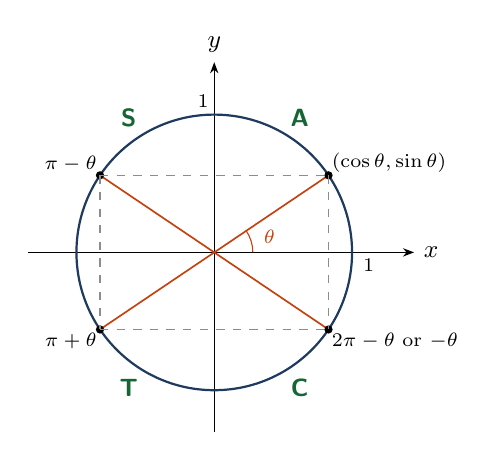
\begin{tikzpicture}[scale=1.75]
  \draw[-{Stealth[length=4pt]}] (-1.35,0) -- (1.45,0) node[right,font=\small] {$x$};
  \draw[-{Stealth[length=4pt]}] (0,-1.3) -- (0,1.38) node[above,font=\small] {$y$};
  \draw[navy, line width=0.8pt] (0,0) circle (1);
  \def\t{34}
  \coordinate (P) at ({cos(\t)},{sin(\t)});
  \coordinate (Q) at ({-cos(\t)},{sin(\t)});
  \coordinate (Rr) at ({-cos(\t)},{-sin(\t)});
  \coordinate (S) at ({cos(\t)},{-sin(\t)});
  \foreach \c in {P,Q,Rr,S} {\draw[plotB, line width=0.6pt] (0,0) -- (\c); \fill (\c) circle (0.03);}
  \draw[dashed, black!45] (Q) -- (P) (Rr) -- (S) (P) -- (S) (Q) -- (Rr);
  \draw[plotB] (0.28,0) arc (0:\t:0.28); \node[font=\scriptsize, plotB] at (0.40,0.11) {$\theta$};
  \node[font=\scriptsize, anchor=south west, inner sep=1pt] at (P) {$(\cos\theta,\sin\theta)$};
  \node[font=\scriptsize, anchor=south east, inner sep=1pt] at (Q) {$\pi-\theta$};
  \node[font=\scriptsize, anchor=north east, inner sep=1pt] at (Rr) {$\pi+\theta$};
  \node[font=\scriptsize, anchor=north west, inner sep=1pt] at (S) {$2\pi-\theta$ or $-\theta$};
  \node[font=\sffamily\bfseries\small, excol] at (0.62,0.98) {A};
  \node[font=\sffamily\bfseries\small, excol] at (-0.62,0.98) {S};
  \node[font=\sffamily\bfseries\small, excol] at (-0.62,-0.98) {T};
  \node[font=\sffamily\bfseries\small, excol] at (0.62,-0.98) {C};
  \node[font=\scriptsize] at (1.12,-0.09) {$1$};
  \node[font=\scriptsize] at (-0.08,1.1) {$1$};
\end{tikzpicture}

{\scriptsize\textbf{A}ll positive in quadrant 1, \textbf{S}in in quadrant 2, \textbf{T}an in quadrant 3, \textbf{C}os in quadrant 4.}
\end{minipage}\hfill
\begin{minipage}[t]{0.5\linewidth}
\vspace{0pt}
\begin{keyres}{Definitions \& identities}
\small
\begin{itemize}
  \item $\pi$ radians $=180^\circ$; \ degrees $\to$ radians: $\times\frac{\pi}{180}$.
  \item Point at angle $\theta$ on the unit circle: $(\cos\theta,\sin\theta)$; \ $\tan\theta=\dfrac{\sin\theta}{\cos\theta}$.
  \item $\sin^2\theta+\cos^2\theta=1$.
  \item $\sin(\pi-\theta)=\sin\theta$, \ $\cos(\pi-\theta)=-\cos\theta$
  \item $\sin(\pi+\theta)=-\sin\theta$, \ $\cos(\pi+\theta)=-\cos\theta$
  \item $\sin(2\pi-\theta)=-\sin\theta$, \ $\cos(2\pi-\theta)=\cos\theta$
  \item $\sin(-\theta)=-\sin\theta$ (odd), \ $\cos(-\theta)=\cos\theta$ (even), \ $\tan(-\theta)=-\tan\theta$
  \item $\tan(\pi\pm\theta)=\pm\tan\theta$ (period $\pi$)
  \item $\sin\!\left(\frac{\pi}{2}-\theta\right)=\cos\theta$, \ $\cos\!\left(\frac{\pi}{2}-\theta\right)=\sin\theta$
\end{itemize}
\end{keyres}
\end{minipage}

\begin{center}
\small
\begin{tabular}{>{\columncolor{keybg}}c|ccccc|cccc}
\toprule
$\theta$ & $0$ & $\frac{\pi}{6}$ ($30^\circ$) & $\frac{\pi}{4}$ ($45^\circ$) & $\frac{\pi}{3}$ ($60^\circ$) & $\frac{\pi}{2}$ ($90^\circ$) & $\pi$ & $\frac{3\pi}{2}$ & $2\pi$ \\
\midrule
$\sin\theta$ & $0$ & $\frac12$ & $\frac{\sqrt2}{2}$ & $\frac{\sqrt3}{2}$ & $1$ & $0$ & $-1$ & $0$\\[2pt]
$\cos\theta$ & $1$ & $\frac{\sqrt3}{2}$ & $\frac{\sqrt2}{2}$ & $\frac12$ & $0$ & $-1$ & $0$ & $1$\\[2pt]
$\tan\theta$ & $0$ & $\frac{1}{\sqrt3}=\frac{\sqrt3}{3}$ & $1$ & $\sqrt3$ & undefined & $0$ & undefined & $0$\\
\bottomrule
\end{tabular}
\end{center}

\begin{tip}[Getting the related angles fast]
For $\frac{\pi}{6}$-type angles, the related angles in $[0,2\pi]$ are $\frac{\pi}{6},\ \frac{5\pi}{6},\ \frac{7\pi}{6},\ \frac{11\pi}{6}$. For $\frac{\pi}{4}$: $\frac{\pi}{4},\frac{3\pi}{4},\frac{5\pi}{4},\frac{7\pi}{4}$. For $\frac{\pi}{3}$: $\frac{\pi}{3},\frac{2\pi}{3},\frac{4\pi}{3},\frac{5\pi}{3}$. Pick the ones in the quadrants where the sign is right (ASTC). Example: $\cos\theta=-\frac{\sqrt3}{2}$ is negative in quadrants 2 and 3, so $\theta=\frac{5\pi}{6},\frac{7\pi}{6}$.
\end{tip}

\subsection{Probability toolkit}

\begin{cols}
\begin{keyres}{Rules}
\small
\begin{itemize}
  \item $0\le\Pr(A)\le1$; \ $\Pr(A')=1-\Pr(A)$.
  \item $\Pr(A\cup B)=\Pr(A)+\Pr(B)-\Pr(A\cap B)$.
  \item Mutually exclusive: $\Pr(A\cap B)=0$.
  \item Conditional: $\Pr(A|B)=\dfrac{\Pr(A\cap B)}{\Pr(B)}$, so $\Pr(A\cap B)=\Pr(A|B)\Pr(B)$.
  \item \textbf{Independent} $\iff\Pr(A\cap B)=\Pr(A)\Pr(B)$ $\iff\Pr(A|B)=\Pr(A)$.
  \item Total probability: $\Pr(A)=\Pr(A|B)\Pr(B)+\Pr(A|B')\Pr(B')$.
  \item Combinations: $\binom{n}{r}={}^nC_r=\dfrac{n!}{r!\,(n-r)!}$; $\binom{n}{0}=\binom{n}{n}=1$, $\binom{n}{1}=n$, $\binom{n}{r}=\binom{n}{n-r}$.
\end{itemize}
\end{keyres}
\nextcol
\begin{keyres}{Karnaugh map (probability table)}
\small
\centering
\begin{tabular}{c|cc|c}
 & $B$ & $B'$ & \\ \hline
$A$ & $\Pr(A\cap B)$ & $\Pr(A\cap B')$ & $\Pr(A)$\\
$A'$ & $\Pr(A'\cap B)$ & $\Pr(A'\cap B')$ & $\Pr(A')$\\ \hline
 & $\Pr(B)$ & $\Pr(B')$ & $1$
\end{tabular}
\par\smallskip\raggedright
Rows and columns add up. Fill in what you know, then complete by subtraction.\par
\textbf{Pascal's triangle} gives $\binom{n}{r}$: row 4 is $1\ 4\ 6\ 4\ 1$; row 5 is $1\ 5\ 10\ 10\ 5\ 1$; row 6 is $1\ 6\ 15\ 20\ 15\ 6\ 1$.
\end{keyres}
\end{cols}

\begin{example}{tree diagram and conditional probability \byhand}
The probability that it rains on a given day is $0.3$. If it rains, Sam is late with probability $0.4$; if it doesn't rain, Sam is late with probability $0.1$. Find $\Pr(\text{late})$ and $\Pr(\text{rain}\mid\text{late})$.

\textbf{Solution.} $\Pr(L)=\Pr(L|R)\Pr(R)+\Pr(L|R')\Pr(R')=0.4(0.3)+0.1(0.7)=0.12+0.07=0.19$.\quad
$\Pr(R|L)=\dfrac{\Pr(R\cap L)}{\Pr(L)}=\dfrac{0.12}{0.19}=\dfrac{12}{19}$.
\end{example}

\begin{example}{independence test \byhand}
$\Pr(A)=0.5$, $\Pr(B)=0.4$, $\Pr(A\cap B)=0.2$. Since $\Pr(A)\Pr(B)=0.2=\Pr(A\cap B)$, $A$ and $B$ \textbf{are independent}. Also $\Pr(A\cup B)=0.5+0.4-0.2=0.7$ and $\Pr(A'\cap B')=1-0.7=0.3$.
\end{example}

% =================================================================
\section{Functions, relations and graphs (Area of Study 1)}
\label{sec:functions}
% =================================================================

\begin{sdbox}
\textbf{This area of study includes:}
\begin{itemize}
  \item graphs of polynomial functions and their key features
  \item graphs of power functions $y=x^n$, $n\in\Q$; exponential functions $y=a^x$, $a\in\R^+$, in particular $y=e^x$; logarithmic functions $y=\loge(x)$ and $y=\log_{10}(x)$; and circular functions $y=\sin(x)$, $y=\cos(x)$ and $y=\tan(x)$, and their key features
  \item transformation from $y=f(x)$ to $y=Af(n(x+b))+c$, where $A,n,b,c\in\R$, $A,n\ne0$, and $f$ is one of the functions above, and the inverse transformation
  \item the relation between the graph of an original function and the graph of a transformed function (including \emph{families} of transformed functions for a single transformation parameter)
  \item graphs of sum, difference, product and composite functions of the types above (not composites that give reciprocal or quotient functions)
  \item modelling of practical situations using polynomial, power, circular, exponential and logarithmic functions, simple transformations and combinations of these, including simple piecewise (hybrid) functions
\end{itemize}
\textbf{Key skill:} \byhand\ sketch graphs of polynomials up to degree 4; $y=x^n$, $n\in\N$; $y=a^x$ (using key points $\left(-1,\frac1a\right)$, $(0,1)$, $(1,a)$); $\loge(x)$; $\log_{10}(x)$; and simple transformations of these, \emph{clearly identifying key features including any vertical or horizontal asymptotes}. Also: domain, maximal domain, co-domain, range, asymptotic behaviour, symmetry, and recognising possible models from graphs or tables.
\end{sdbox}

\subsection{Functions, domain and range}
\label{sec:domain}

\begin{defn}{Definitions}
\begin{itemize}
  \item A \textbf{relation} is a set of ordered pairs. A \textbf{function} is a relation where each $x$-value maps to \emph{exactly one} $y$-value (passes the \emph{vertical line test}).
  \item \textbf{One-to-one}: each $y$-value comes from exactly one $x$-value (passes the \emph{horizontal line test}). Otherwise \textbf{many-to-one} (e.g.\ $y=x^2$ on $\R$). A function has an inverse \emph{function} only if it is one-to-one.
  \item $f:D\to\R,\ f(x)=\text{rule}$. The \textbf{domain} $D$ is the set of allowed inputs; the \textbf{co-domain} ($\R$ in Methods) contains all outputs; the \textbf{range} is the set of outputs actually produced.
  \item The \textbf{maximal} (implied or natural) domain is the largest subset of $\R$ for which the rule is defined. When a function is given by a rule only, assume the maximal domain.
  \item \textbf{Even}: $f(-x)=f(x)$, so the graph is symmetric about the $y$-axis ($x^2$, $x^4$, $\cos x$, $\frac{1}{x^2}$). \textbf{Odd}: $f(-x)=-f(x)$, so the graph has rotational symmetry about the origin ($x^3$, $\frac1x$, $\sin x$, $\tan x$, $x^{1/3}$).
\end{itemize}
\end{defn}

\begin{cols}
\begin{keyres}{Finding the maximal domain}
\begin{itemize}
  \item Denominator $\ne0$.
  \item Even root $\sqrt{\ \ }$: inside $\ge0$.
  \item $\loge(\ \ )$: inside $>0$.
  \item $\tan(\theta)$: $\theta\ne\frac{\pi}{2}+k\pi$, $k\in\Z$.
  \item Sum, difference, product: \emph{intersection} of the domains, $d_{f\pm g}=d_{fg}=d_f\cap d_g$.
\end{itemize}
\end{keyres}
\nextcol
\begin{keyres}{Finding the range}
\begin{itemize}
  \item Sketch it. Read off from the lowest to the highest $y$-value, using endpoints, turning points and asymptotes.
  \item Check endpoints: closed ($\bullet$, included) or open ($\circ$, excluded).
  \item Asymptotes are \emph{never} included in the range ($y=e^x$ has range $(0,\infty)$).
\end{itemize}
\end{keyres}
\end{cols}

\begin{example}{maximal domain and range \byhand}
\begin{tabularx}{\linewidth}{@{}p{3.8cm}L@{}}
$f(x)=\sqrt{4-2x}+1$ & Need $4-2x\ge0\Rightarrow x\le2$. Domain $(-\infty,2]$; range $[1,\infty)$ (endpoint $(2,1)$). \\
$g(x)=\loge(3-x)-2$ & Need $3-x>0\Rightarrow x<3$. Domain $(-\infty,3)$; range $\R$; vertical asymptote $x=3$; $x$-intercept $3-e^2$; $y$-intercept $\loge3-2$. \\
$h(x)=\dfrac{2}{(x-1)^2}-3$ & Domain $\R\setminus\{1\}$; asymptotes $x=1$, $y=-3$; range $(-3,\infty)$. \\
\end{tabularx}
\end{example}

\begin{tip}[Key features checklist for any sketch]
Axis intercepts (as coordinates) \textbullet\ stationary points and their nature \textbullet\ points of inflection (if asked) \textbullet\ asymptotes as dashed lines \emph{with equations} \textbullet\ endpoints shown closed $\bullet$ or open $\circ$ with coordinates \textbullet\ correct behaviour near asymptotes and as $x\to\pm\infty$ \textbullet\ correct curvature (don't draw a parabola-shaped log graph) \textbullet\ symmetry used where possible.
\end{tip}

% -----------------------------------------------------------------
\subsection{Polynomial functions}
\label{sec:poly}

\begin{keyres}{Shape rules for polynomials of degree $n$}
\begin{itemize}
  \item At most $n$ $x$-intercepts and at most $n-1$ turning points. The $y$-intercept is the constant term.
  \item \textbf{Behaviour at a root} $x=a$ from a factor $(x-a)^k$: $k=1$ the graph \emph{crosses}; $k=2$ it \emph{touches} (turning point on the axis); $k=3$ it crosses with a \emph{stationary point of inflection} (flattens).
  \item \textbf{End behaviour} (leading term $ax^n$ dominates): $n$ even, $a>0$: up at both ends; $n$ even, $a<0$: down at both ends; $n$ odd, $a>0$: bottom left to top right; $n$ odd, $a<0$: top left to bottom right.
  \item Turning-point (stationary-point) forms: $y=a(x-h)^2+k$ and $y=a(x-h)^4+k$ have a turning point at $(h,k)$; $y=a(x-h)^3+k$ has a stationary point of inflection at $(h,k)$.
  \item Comparing powers: for $|x|<1$, $x^4<x^2$ (flatter near $0$); for $|x|>1$, $x^4>x^2$. All of $x^2,x^4$ pass through $(-1,1),(0,0),(1,1)$; $x^3,x^5$ through $(-1,-1),(0,0),(1,1)$.
\end{itemize}
\end{keyres}

\begin{cols}
\begin{example}{a cubic \byhand}
Sketch $y=(x+1)^2(x-2)$.\par
\textbf{Intercepts:} touches at $x=-1$, crosses at $x=2$; $y$-intercept $(1)^2(-2)=-2$.\par
\textbf{Stationary points:} $\dydx=2(x+1)(x-2)+(x+1)^2=3(x+1)(x-1)$, so local max $(-1,0)$ and local min $(1,-4)$.\par
\textbf{Ends:} degree 3, positive leading coefficient: bottom left to top right.
\end{example}
\nextcol
\centering
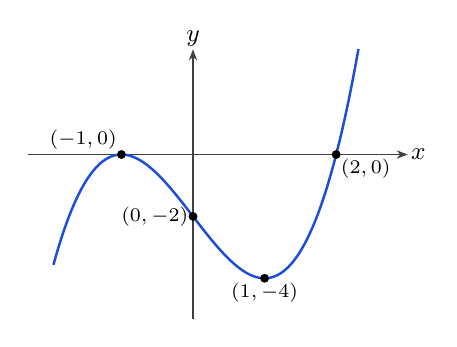
\begin{tikzpicture}
\begin{axis}[mygraph, width=6.4cm, height=5.0cm, xmin=-2.3, xmax=3.0, ymin=-5.3, ymax=3.4, xtick=\empty, ytick=\empty]
  \addplot[plotA, domain=-1.95:2.45] {(x+1)^2*(x-2)};
  \node[pt] at (axis cs:-1,0) {}; \node[lab, above left] at (axis cs:-1,0) {$(-1,0)$};
  \node[pt] at (axis cs:1,-4) {}; \node[lab, below] at (axis cs:1,-4) {$(1,-4)$};
  \node[pt] at (axis cs:2,0) {};  \node[lab, below right] at (axis cs:2,0) {$(2,0)$};
  \node[pt] at (axis cs:0,-2) {}; \node[lab, left] at (axis cs:0,-2) {$(0,-2)$};
\end{axis}
\end{tikzpicture}
\end{cols}

\begin{cols}
\begin{example}{a quartic \byhand}
Sketch $y=x(x-2)^3$.\par
\textbf{Intercepts:} crosses at $(0,0)$; at $x=2$ (triple root) a stationary point of inflection.\par
\textbf{Stationary points:} $\dydx=(x-2)^3+3x(x-2)^2=(x-2)^2(4x-2)$: $x=\frac12$ gives the local min $\left(\frac12,-\frac{27}{16}\right)$; $x=2$ gives the stationary inflection $(2,0)$.\par
\textbf{Ends:} degree 4, $a>0$: up at both ends.
\end{example}
\nextcol
\centering
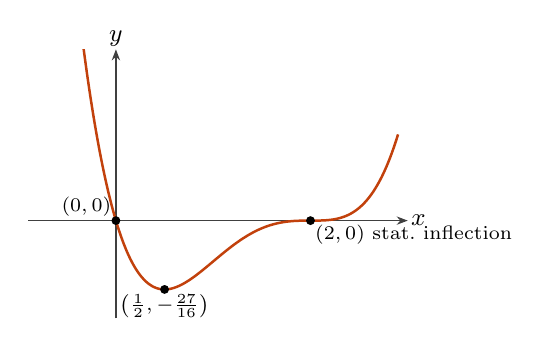
\begin{tikzpicture}
\begin{axis}[mygraph, width=6.4cm, height=5.0cm, xmin=-0.9, xmax=3.0, ymin=-2.4, ymax=4.2, xtick=\empty, ytick=\empty]
  \addplot[plotB, domain=-0.42:2.9] {x*(x-2)^3};
  \node[pt] at (axis cs:0,0) {}; \node[lab, above left] at (axis cs:0,0) {$(0,0)$};
  \node[pt] at (axis cs:0.5,-1.6875) {}; \node[lab, below] at (axis cs:0.5,-1.6875) {$\left(\frac12,-\frac{27}{16}\right)$};
  \node[pt] at (axis cs:2,0) {}; \node[lab, below right] at (axis cs:2,0) {$(2,0)$ stat.\ inflection};
\end{axis}
\end{tikzpicture}
\end{cols}

% -----------------------------------------------------------------
\subsection{Power functions $y=x^n$, $n\in\Q$}
\label{sec:power}

\begin{center}
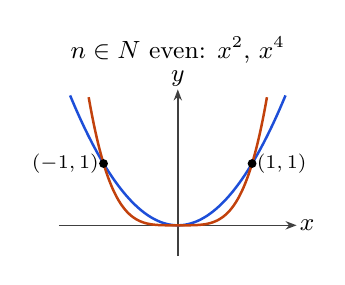
\begin{tikzpicture}
\begin{axis}[smallgraph, title={\small $n\in\N$ even: $x^2$, $x^4$}, xmin=-1.6, xmax=1.6, ymin=-0.5, ymax=2.2, xtick=\empty, ytick=\empty]
  \addplot[plotA, domain=-1.45:1.45] {x^2};
  \addplot[plotB, domain=-1.2:1.2] {x^4};
  \node[pt] at (axis cs:1,1) {}; \node[lab, right] at (axis cs:1,1) {$(1,1)$};
  \node[pt] at (axis cs:-1,1) {}; \node[lab, left] at (axis cs:-1,1) {$(-1,1)$};
\end{axis}
\end{tikzpicture}\hfill
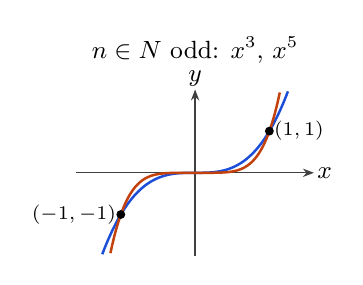
\begin{tikzpicture}
\begin{axis}[smallgraph, title={\small $n\in\N$ odd: $x^3$, $x^5$}, xmin=-1.6, xmax=1.6, ymin=-2, ymax=2, xtick=\empty, ytick=\empty]
  \addplot[plotA, domain=-1.25:1.25] {x^3};
  \addplot[plotB, domain=-1.14:1.14] {x^5};
  \node[pt] at (axis cs:1,1) {}; \node[lab, right] at (axis cs:1,1) {$(1,1)$};
  \node[pt] at (axis cs:-1,-1) {}; \node[lab, left] at (axis cs:-1,-1) {$(-1,-1)$};
\end{axis}
\end{tikzpicture}\hfill
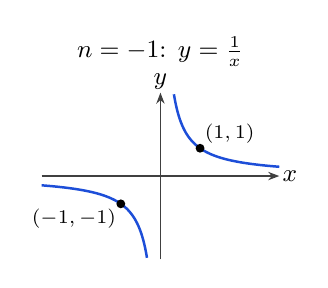
\begin{tikzpicture}
\begin{axis}[smallgraph, title={\small $n=-1$: $y=\frac1x$}, xmin=-3, xmax=3, ymin=-3, ymax=3, xtick=\empty, ytick=\empty]
  \addplot[plotA, domain=-3:-0.34] {1/x};
  \addplot[plotA, domain=0.34:3] {1/x};
  \node[pt] at (axis cs:1,1) {}; \node[lab, above right] at (axis cs:1,1) {$(1,1)$};
  \node[pt] at (axis cs:-1,-1) {}; \node[lab, below left] at (axis cs:-1,-1) {$(-1,-1)$};
\end{axis}
\end{tikzpicture}

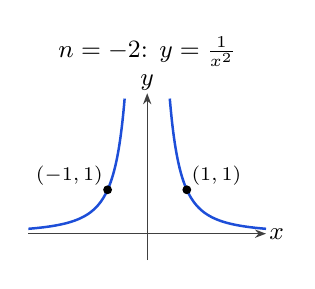
\begin{tikzpicture}
\begin{axis}[smallgraph, title={\small $n=-2$: $y=\frac{1}{x^2}$}, xmin=-3, xmax=3, ymin=-0.6, ymax=3.2, xtick=\empty, ytick=\empty]
  \addplot[plotA, domain=-3:-0.57] {1/x^2};
  \addplot[plotA, domain=0.57:3] {1/x^2};
  \node[pt] at (axis cs:1,1) {}; \node[lab, above right] at (axis cs:1,1) {$(1,1)$};
  \node[pt] at (axis cs:-1,1) {}; \node[lab, above left] at (axis cs:-1,1) {$(-1,1)$};
\end{axis}
\end{tikzpicture}\hfill
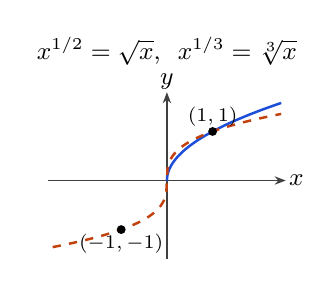
\begin{tikzpicture}
\begin{axis}[smallgraph, title={\small $x^{1/2}=\sqrt{x}$,\ \ $x^{1/3}=\sqrt[3]{x}$}, xmin=-2.6, xmax=2.6, ymin=-1.6, ymax=1.8, xtick=\empty, ytick=\empty]
  \addplot[plotA, domain=0:2.5, samples=300] {sqrt(x)};
  \addplot[plotB, dashed, domain=-2.5:2.5] {sign(x)*abs(x)^(1/3)};
  \node[pt] at (axis cs:1,1) {}; \node[lab, above] at (axis cs:1,1) {$(1,1)$};
  \node[pt] at (axis cs:-1,-1) {}; \node[lab, below] at (axis cs:-1,-1) {$(-1,-1)$};
\end{axis}
\end{tikzpicture}\hfill
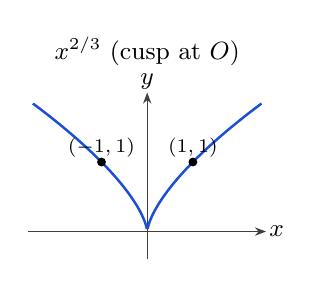
\begin{tikzpicture}
\begin{axis}[smallgraph, title={\small $x^{2/3}$ (cusp at $O$)}, xmin=-2.6, xmax=2.6, ymin=-0.4, ymax=2.0, xtick=\empty, ytick=\empty]
  \addplot[plotA, domain=-2.5:2.5] {abs(x)^(2/3)};
  \node[pt] at (axis cs:1,1) {}; \node[lab, above] at (axis cs:1,1) {$(1,1)$};
  \node[pt] at (axis cs:-1,1) {}; \node[lab, above] at (axis cs:-1,1) {$(-1,1)$};
\end{axis}
\end{tikzpicture}
\end{center}

\begin{center}
\small
\begin{tabularx}{\linewidth}{@{}lllL@{}}
\toprule
$y=x^n$ & Maximal domain & Range & Notes \\
\midrule
$n\in\N$ even ($x^2,x^4$) & $\R$ & $[0,\infty)$ & even; turning point at $O$ \\
$n\in\N$ odd ($x^3,x^5$) & $\R$ & $\R$ & odd; stationary inflection at $O$ ($n\ge3$) \\
$n=-1$, $\frac1x$ (hyperbola) & $\R\setminus\{0\}$ & $\R\setminus\{0\}$ & odd; asymptotes $x=0$, $y=0$ \\
$n=-2$, $\frac{1}{x^2}$ (truncus) & $\R\setminus\{0\}$ & $(0,\infty)$ & even; asymptotes $x=0$, $y=0$ \\
$n=\frac12$, $\sqrt{x}$ & $[0,\infty)$ & $[0,\infty)$ & starts at $(0,0)$; vertical tangent there \\
$n=\frac13$, $\sqrt[3]{x}$ & $\R$ & $\R$ & odd; vertical tangent at $O$ (not differentiable at $0$) \\
$n=\frac23$, $\left(\sqrt[3]{x}\right)^2$ & $\R$ & $[0,\infty)$ & even; cusp at $O$ \\
$n=-\frac12$, $\frac{1}{\sqrt{x}}$ & $(0,\infty)$ & $(0,\infty)$ & asymptotes $x=0$, $y=0$ \\
\bottomrule
\end{tabularx}
\end{center}

\begin{keyres}{General rational powers and transformed power functions}
For $n=\frac{p}{q}$ in simplest form ($q>0$): $x^{p/q}=\left(\sqrt[q]{x}\right)^p$. If $q$ is \textbf{odd}, negative $x$ is allowed; if $q$ is \textbf{even}, need $x\ge0$. If $p<0$, also exclude $x=0$. Every $y=x^n$ passes through $(1,1)$.
\begin{itemize}
  \item $y=\dfrac{a}{x-h}+k$ and $y=\dfrac{a}{(x-h)^2}+k$: asymptotes $x=h$ and $y=k$.
  \item $y=a\sqrt{x-h}+k$: starts at $(h,k)$, domain $[h,\infty)$; $y=a\sqrt{h-x}+k$ has domain $(-\infty,h]$.
\end{itemize}
\end{keyres}

% -----------------------------------------------------------------
\subsection{Exponential and logarithmic functions}
\label{sec:explog}

\begin{cols}
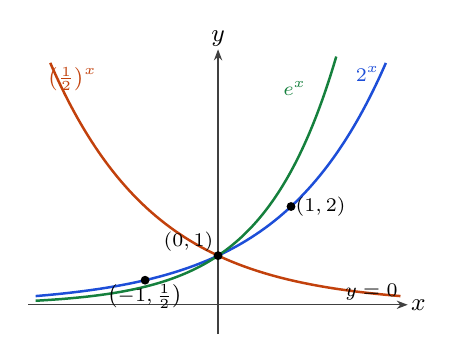
\begin{tikzpicture}
\begin{axis}[mygraph, width=6.4cm, height=5.2cm, xmin=-2.6, xmax=2.6, ymin=-0.6, ymax=5.2, xtick=\empty, ytick=\empty]
  \addplot[plotA, domain=-2.5:2.3] {2^x};
  \addplot[plotC, domain=-2.5:1.62] {exp(x)};
  \addplot[plotB, domain=-2.3:2.5] {0.5^x};
  \node[pt] at (axis cs:0,1) {}; \node[lab, above left] at (axis cs:0,1) {$(0,1)$};
  \node[pt] at (axis cs:1,2) {}; \node[lab, right] at (axis cs:1,2) {$(1,2)$};
  \node[pt] at (axis cs:-1,0.5) {}; \node[lab, below] at (axis cs:-1,0.5) {$\left(-1,\frac12\right)$};
  \node[lab, plotA] at (axis cs:2.05,4.7) {$2^x$};
  \node[lab, plotC] at (axis cs:1.05,4.4) {$e^x$};
  \node[lab, plotB] at (axis cs:-2.0,4.6) {$\left(\frac12\right)^x$};
  \node[lab] at (axis cs:2.1,0.25) {$y=0$};
\end{axis}
\end{tikzpicture}
\nextcol
\begin{keyres}{$y=a^x$, $a>0$, $a\ne1$}
\begin{itemize}
  \item Domain $\R$; range $(0,\infty)$; horizontal asymptote $y=0$.
  \item Key points $\left(-1,\frac1a\right)$, $(0,1)$, $(1,a)$.
  \item $a>1$: strictly increasing (growth). $0<a<1$: strictly decreasing (decay). $\left(\frac1a\right)^x=a^{-x}$ is the reflection in the $y$-axis.
  \item $e\approx2.718$. $y=e^x$ has gradient $1$ at $(0,1)$ and $\ddx e^x=e^x$.
  \item $y=Ae^{n(x-h)}+k$: asymptote $y=k$; range $(k,\infty)$ if $A>0$, $(-\infty,k)$ if $A<0$.
\end{itemize}
\end{keyres}
\end{cols}

\begin{cols}
\begin{keyres}{$y=\log_a(x)$: the inverse of $y=a^x$}
\begin{itemize}
  \item $y=\log_a(x)\iff a^y=x$ (for $x>0$).
  \item Domain $(0,\infty)$; range $\R$; vertical asymptote $x=0$.
  \item Key points $\left(\frac1a,-1\right)$, $(1,0)$, $(a,1)$; reflection of $y=a^x$ in $y=x$.
  \item $\loge(x)=\ln(x)$ passes through $(e,1)$; $\log_{10}(x)$ through $(10,1)$, flatter than $\loge$ for $x>1$.
  \item $y=A\loge(n(x-h))+k$: asymptote $x=h$; domain $x>h$ if $n>0$, $x<h$ if $n<0$.
\end{itemize}
\end{keyres}
\nextcol
\centering
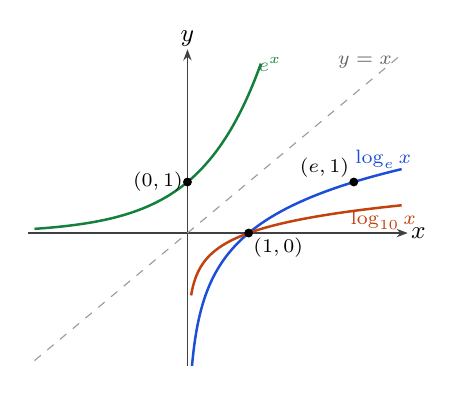
\begin{tikzpicture}
\begin{axis}[mygraph, width=6.4cm, height=5.6cm, xmin=-2.6, xmax=3.6, ymin=-2.6, ymax=3.6, xtick=\empty, ytick=\empty]
  \addplot[black!40, dashed, thin, domain=-2.5:3.5] {x};
  \addplot[plotC, domain=-2.5:1.2] {exp(x)};
  \addplot[plotA, domain=0.07:3.5, samples=300] {ln(x)};
  \addplot[plotB, domain=0.06:3.5, samples=300] {log10(x)};
  \node[pt] at (axis cs:1,0) {}; \node[lab, below right] at (axis cs:1,0) {$(1,0)$};
  \node[pt] at (axis cs:2.71828,1) {}; \node[lab, above left] at (axis cs:2.71828,1) {$(e,1)$};
  \node[pt] at (axis cs:0,1) {}; \node[lab, left] at (axis cs:0,1) {$(0,1)$};
  \node[lab, plotC] at (axis cs:1.35,3.3) {$e^x$};
  \node[lab, plotA] at (axis cs:3.2,1.45) {$\loge x$};
  \node[lab, plotB] at (axis cs:3.2,0.25) {$\log_{10}x$};
  \node[lab, black!60] at (axis cs:2.9,3.35) {$y=x$};
\end{axis}
\end{tikzpicture}
\end{cols}

\begin{keyres}{Index laws and logarithm laws (memorise)}
\begin{cols}
\textbf{Index laws} ($a,b>0$)
\begin{itemize}
  \item $a^ma^n=a^{m+n}$, \ $\dfrac{a^m}{a^n}=a^{m-n}$, \ $(a^m)^n=a^{mn}$
  \item $(ab)^n=a^nb^n$, \ $a^0=1$, \ $a^{-n}=\dfrac{1}{a^n}$
  \item $a^{p/q}=\sqrt[q]{a^p}=\left(\sqrt[q]{a}\right)^p$
  \item $a^{x}=e^{x\loge a}$ (useful for calculus)
\end{itemize}
\nextcol
\textbf{Logarithm laws} ($a>0$, $a\ne1$, $m,n>0$)
\begin{itemize}
  \item $\log_a(mn)=\log_a m+\log_a n$; \ $\log_a\!\left(\frac{m}{n}\right)=\log_a m-\log_a n$
  \item $\log_a(m^p)=p\log_a m$; \ $\log_a\!\left(\frac1m\right)=-\log_a m$
  \item $\log_a1=0$, \ $\log_a a=1$, \ $a^{\log_a x}=x$, \ $\log_a(a^x)=x$
  \item Change of base: $\log_a x=\dfrac{\loge x}{\loge a}$
\end{itemize}
\end{cols}
\end{keyres}

\begin{warn}
$\log_a(m+n)\ne\log_a m+\log_a n$ \textbullet\ $\dfrac{\log m}{\log n}\ne\log\!\left(\dfrac mn\right)$ \textbullet\ $(\loge x)^2\ne2\loge x$ \textbullet\ $\loge(x^2)=2\loge|x|$, so $\loge(x^2)$ and $2\loge x$ have \emph{different domains} \textbullet\ $e^{a+b}=e^ae^b$, not $e^a+e^b$.
\end{warn}

\begin{example}{sketching transformed exponential and log graphs \byhand}
\textbf{(a)} $y=3-e^{2x}$: asymptote $y=3$ (as $x\to-\infty$); $y$-intercept $3-1=2$; $x$-intercept $e^{2x}=3\Rightarrow x=\frac12\loge3$; range $(-\infty,3)$; strictly decreasing.\par
\textbf{(b)} $y=\loge(3-x)-2$ (from the earlier domain example): reflect $y=\loge x$ in the $y$-axis, translate 3 right, 2 down. Asymptote $x=3$; $x$-intercept $3-e^2\approx-4.39$; $y$-intercept $\loge3-2\approx-0.90$; domain $(-\infty,3)$; strictly decreasing.
\end{example}

% -----------------------------------------------------------------
\subsection{Circular functions}
\label{sec:circ}

\begin{cols}
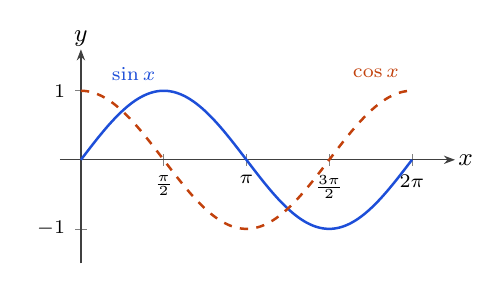
\begin{tikzpicture}
\begin{axis}[mygraph, width=6.6cm, height=4.3cm, xmin=-0.4, xmax=7.1, ymin=-1.5, ymax=1.6,
  xtick={1.5708,3.14159,4.71239,6.28319}, xticklabels={$\frac{\pi}{2}$,$\pi$,$\frac{3\pi}{2}$,$2\pi$},
  ytick={-1,1}, every tick label/.append style={font=\scriptsize}]
  \addplot[plotA, domain=0:6.28319] {sin(deg(x))};
  \addplot[plotB, dashed, domain=0:6.28319] {cos(deg(x))};
  \node[lab, plotA] at (axis cs:1.0,1.25) {$\sin x$};
  \node[lab, plotB] at (axis cs:5.6,1.25) {$\cos x$};
\end{axis}
\end{tikzpicture}

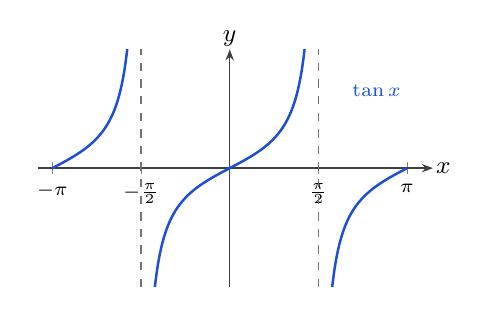
\begin{tikzpicture}
\begin{axis}[mygraph, width=6.6cm, height=4.6cm, xmin=-3.4, xmax=3.6, ymin=-4, ymax=4,
  xtick={-3.14159,-1.5708,1.5708,3.14159}, xticklabels={$-\pi$,$-\frac{\pi}{2}$,$\frac{\pi}{2}$,$\pi$}, ytick=\empty,
  restrict y to domain=-6:6, unbounded coords=jump]
  \addplot[plotA, domain=-3.14159:3.14159, samples=401] {tan(deg(x))};
  \asym (axis cs:-1.5708,-4) -- (axis cs:-1.5708,4);
  \asym (axis cs:1.5708,-4) -- (axis cs:1.5708,4);
  \node[lab, plotA] at (axis cs:2.6,2.6) {$\tan x$};
\end{axis}
\end{tikzpicture}
\nextcol
\begin{keyres}{Key features}
\begin{itemize}
  \item $\sin$, $\cos$: domain $\R$, range $[-1,1]$, period $2\pi$. $\cos x=\sin\!\left(x+\frac{\pi}{2}\right)$.
  \item $\tan$: period $\pi$; asymptotes $x=\frac{\pi}{2}+k\pi$; zeros at $x=k\pi$; range $\R$.
  \item $y=a\sin(n(x-b))+c$ or $a\cos(n(x-b))+c$:\\
   amplitude $|a|$; \ period $\dfrac{2\pi}{|n|}$; \ mean line $y=c$; \ range $[c-|a|,\,c+|a|]$; \ horizontal shift $b$.
  \item $y=a\tan(n(x-b))+c$: period $\dfrac{\pi}{|n|}$; asymptotes where $n(x-b)=\frac{\pi}{2}+k\pi$, i.e.\ $x=b+\dfrac{\pi}{2n}+\dfrac{k\pi}{n}$, $k\in\Z$.
\end{itemize}
\end{keyres}
\begin{method}{Sketching $y=a\sin(n(x-b))+c$ \byhand}
\begin{enumerate}
  \item Factorise the inside: $\sin(2x-\frac{\pi}{2})=\sin\!\left(2\left(x-\frac{\pi}{4}\right)\right)$.
  \item Period, amplitude, mean line, range.
  \item Mark a cycle starting at $x=b$ and split it into quarters. The key points are mean, max, mean, min, mean (sin) or max, mean, min, mean, max (cos), flipped if $a<0$.
  \item Find the intercepts by solving; plot the endpoints of the domain.
\end{enumerate}
\end{method}
\end{cols}

\begin{cols}[0.52]
\begin{example}{a transformed circular graph \byhand}
Sketch $y=2\sin\!\left(2x-\frac{\pi}{2}\right)+1$ for $x\in[0,2\pi]$.\par
$y=2\sin\!\left(2\left(x-\frac{\pi}{4}\right)\right)+1$: amplitude $2$, period $\pi$, mean line $y=1$, range $[-1,3]$. It simplifies to $y=1-2\cos(2x)$.\par
$y$-intercept: $2\sin\!\left(-\frac{\pi}{2}\right)+1=-1$.\par
$x$-intercepts: $\cos(2x)=\frac12$, $2x\in[0,4\pi]$, so $2x=\frac{\pi}{3},\frac{5\pi}{3},\frac{7\pi}{3},\frac{11\pi}{3}$, giving $x=\frac{\pi}{6},\frac{5\pi}{6},\frac{7\pi}{6},\frac{11\pi}{6}$.\par
Maxima $\left(\frac{\pi}{2},3\right)$, $\left(\frac{3\pi}{2},3\right)$; minima $(0,-1)$, $(\pi,-1)$, $(2\pi,-1)$.
\end{example}
\nextcol[0.455]
\centering
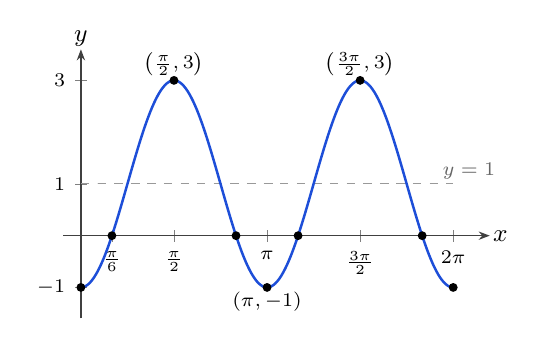
\begin{tikzpicture}
\begin{axis}[mygraph, width=7.0cm, height=5.0cm, xmin=-0.3, xmax=6.9, ymin=-1.6, ymax=3.6,
  xtick={0.5236,1.5708,3.14159,4.71239,6.28319}, xticklabels={$\frac{\pi}{6}$,$\frac{\pi}{2}$,$\pi$,$\frac{3\pi}{2}$,$2\pi$},
  ytick={-1,1,3}, every tick label/.append style={font=\scriptsize}]
  \addplot[black!40, dashed, thin, domain=0:6.28319] {1};
  \addplot[plotA, domain=0:6.28319] {1-2*cos(deg(2*x))};
  \node[pt] at (axis cs:0,-1) {}; \node[pt] at (axis cs:6.28319,-1) {};
  \node[pt] at (axis cs:1.5708,3) {}; \node[lab, above] at (axis cs:1.5708,3) {$\left(\frac{\pi}{2},3\right)$};
  \node[pt] at (axis cs:4.71239,3) {}; \node[lab, above] at (axis cs:4.71239,3) {$\left(\frac{3\pi}{2},3\right)$};
  \node[pt] at (axis cs:3.14159,-1) {}; \node[lab, below] at (axis cs:3.14159,-1) {$(\pi,-1)$};
  \node[pt] at (axis cs:0.5236,0) {}; \node[pt] at (axis cs:2.618,0) {};
  \node[pt] at (axis cs:3.6652,0) {}; \node[pt] at (axis cs:5.7596,0) {};
  \node[lab, black!60] at (axis cs:6.55,1.25) {$y=1$};
\end{axis}
\end{tikzpicture}
\end{cols}

% -----------------------------------------------------------------
\subsection{Transformations of graphs}
\label{sec:trans}

\begin{keyres}{The study design form $y=Af\big(n(x+b)\big)+c$, \ $A,n\ne0$}
\begin{center}
\begin{tabularx}{\linewidth}{@{}lL@{}}
\toprule
Parameter & Effect on the graph of $y=f(x)$ \\
\midrule
$|A|$ & Dilation by factor $|A|$ \textbf{from the $x$-axis} (parallel to the $y$-axis). If $A<0$: also a \textbf{reflection in the $x$-axis}. \\
$|n|$ & Dilation by factor $\dfrac{1}{|n|}$ \textbf{from the $y$-axis} (parallel to the $x$-axis). If $n<0$: also a \textbf{reflection in the $y$-axis}. \\
$b$ & Translation of $b$ units in the \textbf{negative} $x$-direction ($x+3$: 3 units \emph{left}; $x-3$: 3 units \emph{right}). \\
$c$ & Translation of $c$ units in the positive $y$-direction (up if $c>0$). \\
\bottomrule
\end{tabularx}
\end{center}
\textbf{Mapping of points:} \quad $(x,\,y)\ \longrightarrow\ \left(\dfrac{x}{n}-b,\ \ Ay+c\right)$. \quad For this form apply \textbf{dilations and reflections first, then translations}.\par
\textbf{Effect on features:} the image of a point is found with the mapping. A vertical asymptote $x=h$ becomes $x=\frac{h}{n}-b$; a horizontal asymptote $y=k$ becomes $y=Ak+c$; maxima become minima under a reflection in the $x$-axis; domain and range transform with the $x$- and $y$-rules respectively.
\end{keyres}

\begin{method}{Finding the transformations between two rules}
\textbf{Method 1 (read off):} rewrite the image rule as $y=Af(n(x+b))+c$, \emph{taking out the factor $n$ inside the brackets first}, then read off $A$, $n$, $b$, $c$.\par
\textbf{Method 2 (dash method):} let the image of $(x,y)$ be $(x',y')$. Write $x'$ and $y'$ in terms of $x$ and $y$, make $x$ and $y$ the subjects, and substitute into $y=f(x)$. Then drop the dashes. This works for \emph{any} described sequence of transformations, in any order.
\end{method}

\begin{cols}[0.6]
\begin{example}{describe the transformations \byhand}
Find a sequence of transformations that maps $y=\sqrt{x}$ onto $y=3-2\sqrt{4-x}$.\par
Write it as $y=-2\sqrt{-(x-4)}+3$: $A=-2$, $n=-1$, $b=-4$, $c=3$.
\begin{enumerate}
  \item dilation by factor 2 from the $x$-axis;
  \item reflection in the $x$-axis;
  \item reflection in the $y$-axis;
  \item translation 4 units right and 3 units up.
\end{enumerate}
Mapping: $(x,y)\to(4-x,\ 3-2y)$.\par
\textbf{Check (dash method):} $x'=4-x\Rightarrow x=4-x'$, \ $y'=3-2y\Rightarrow y=\frac{3-y'}{2}$. Substitute into $y=\sqrt x$: $\frac{3-y'}{2}=\sqrt{4-x'}$, so $y'=3-2\sqrt{4-x'}$. \tick
\end{example}
\nextcol[0.37]
\centering
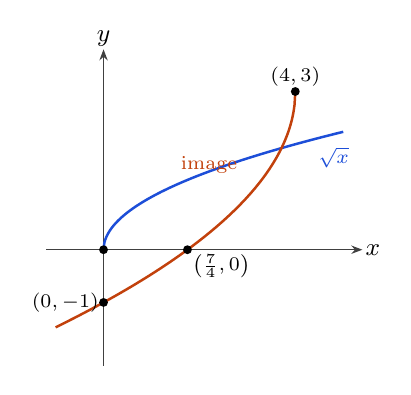
\begin{tikzpicture}
\begin{axis}[mygraph, width=5.6cm, height=5.6cm, xmin=-1.2, xmax=5.4, ymin=-2.2, ymax=3.8, xtick=\empty, ytick=\empty]
  \addplot[plotA, domain=0:5, samples=300] {sqrt(x)};
  \addplot[plotB, domain=-1:4, samples=300] {3-2*sqrt(4-x)};
  \node[pt] at (axis cs:0,0) {};
  \node[pt] at (axis cs:4,3) {}; \node[lab, above] at (axis cs:4,3) {$(4,3)$};
  \node[pt] at (axis cs:1.75,0) {}; \node[lab, below right] at (axis cs:1.75,0) {$\left(\frac74,0\right)$};
  \node[pt] at (axis cs:0,-1) {}; \node[lab, left] at (axis cs:0,-1) {$(0,-1)$};
  \node[lab, plotA] at (axis cs:4.8,1.75) {$\sqrt{x}$};
  \node[lab, plotB] at (axis cs:2.2,1.6) {image};
\end{axis}
\end{tikzpicture}

{\scriptsize The image starts at $(4,3)$ (the image of $(0,0)$) and has domain $(-\infty,4]$ and range $(-\infty,3]$.}
\end{cols}

\begin{example}{image under a mapping; non-uniqueness}
Find the image of $y=\loge(x)$ under $T(x,y)=\left(\frac{x}{3}+2,\ 2y+1\right)$.\par
$x'=\frac x3+2\Rightarrow x=3(x'-2)$; \ $y'=2y+1\Rightarrow y=\frac{y'-1}{2}$. So $\frac{y'-1}{2}=\loge(3(x'-2))$, giving $y=2\loge(3x-6)+1$.\par
\textbf{Non-uniqueness:} by the log laws, $2\loge(3(x-2))+1=2\loge(x-2)+(1+2\loge3)$. So the same graph is obtained \emph{without} any dilation from the $y$-axis: dilate by factor 2 from the $x$-axis, then translate 2 units right and $1+2\loge3$ units up. Exam questions may have several correct answers.\par
\textbf{Inverse transformation:} undo in reverse order. $T^{-1}(x,y)=\left(3(x-2),\ \frac{y-1}{2}\right)$ maps $y=2\loge(3x-6)+1$ back onto $y=\loge x$.
\end{example}

\begin{warn}
\begin{itemize}
  \item \textbf{Order matters.} For $y=x^2$: ``dilate by factor 2 from the $y$-axis, then translate 3 right'' gives $y=\left(\frac{x-3}{2}\right)^2$; ``translate 3 right, then dilate by factor 2 from the $y$-axis'' gives $y=\left(\frac{x}{2}-3\right)^2$. These are different graphs.
  \item $y=f(2x)$ is a dilation by factor $\frac12$ (not 2) from the $y$-axis. In $y=\sin(2x+\pi)=\sin\!\big(2\left(x+\frac{\pi}{2}\right)\big)$ the translation is $\frac{\pi}{2}$ left, not $\pi$.
  \item ``From the $x$-axis'' means vertical stretching. ``Parallel to the $x$-axis'' means horizontal. Read carefully.
\end{itemize}
\end{warn}

\begin{cas}[Transformations seen in other forms]
Exams sometimes write a transformation as a matrix equation:
$T\!\left(\begin{bmatrix}x\\y\end{bmatrix}\right)=\begin{bmatrix}\frac1n&0\\0&A\end{bmatrix}\begin{bmatrix}x\\y\end{bmatrix}+\begin{bmatrix}-b\\c\end{bmatrix}$, which is the same mapping $(x,y)\to\left(\frac xn-b,\ Ay+c\right)$. Read it as ``$x'=\frac{x}{n}-b$, $y'=Ay+c$'' and use the dash method.
\end{cas}

\begin{cols}[0.58]
\begin{keyres}{Families of functions (one parameter)}\label{sec:families}
A \textbf{family} is a set of graphs given by one rule with a parameter, e.g.\ $y=e^{kx}$, $y=kx(x-2)$, $y=x^3-kx$, $y=(x-k)^2+k$.
\begin{itemize}
  \item \textbf{Common points:} find points that do not depend on the parameter. $y=kx(x-2)$ always passes through $(0,0)$ and $(2,0)$; $y=e^{kx}$ through $(0,1)$; $y=k(x-1)+2$ through $(1,2)$.
  \item \textbf{Locus of a feature:} $y=(x-k)^2+k$ has turning point $(k,k)$, which always lies on $y=x$ (see the figure).
  \item \textbf{Conditions on the parameter:} e.g.\ $y=x^3-kx$ has two stationary points only if $k>0$ (they are at $x=\pm\sqrt{k/3}$).
  \item Use CAS to graph several members (Exam 2), then prove the result algebraically.
\end{itemize}
\end{keyres}
\nextcol[0.39]
\centering
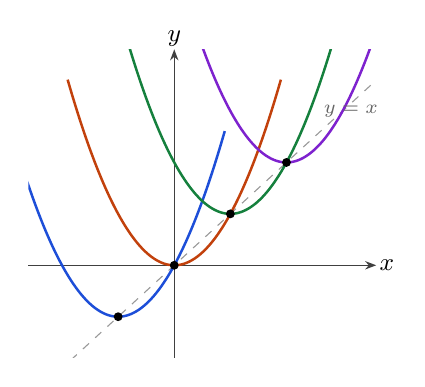
\begin{tikzpicture}
\begin{axis}[mygraph, width=6.0cm, height=5.5cm, xmin=-2.6, xmax=3.6, ymin=-1.8, ymax=4.2, xtick=\empty, ytick=\empty]
  \addplot[black!40, dashed, thin, domain=-2.5:3.5] {x};
  \addplot[plotA, domain=-2.9:0.9] {(x+1)^2-1};
  \addplot[plotB, domain=-1.9:1.9] {x^2};
  \addplot[plotC, domain=-0.9:2.9] {(x-1)^2+1};
  \addplot[plotD, domain=0.1:3.9] {(x-2)^2+2};
  \node[pt] at (axis cs:-1,-1) {}; \node[pt] at (axis cs:0,0) {};
  \node[pt] at (axis cs:1,1) {};   \node[pt] at (axis cs:2,2) {};
  \node[lab, black!60] at (axis cs:3.15,3.0) {$y=x$};
\end{axis}
\end{tikzpicture}

{\scriptsize $y=(x-k)^2+k$ for $k=-1,0,1,2$.}
\end{cols}

% -----------------------------------------------------------------
\subsection{Sums, differences, products and composites of functions}
\label{sec:combo}

\begin{keyres}{Combining functions}
\begin{itemize}
  \item $(f\pm g)(x)=f(x)\pm g(x)$ and $(fg)(x)=f(x)\,g(x)$, each with domain $d_f\cap d_g$.
  \item \textbf{Addition of ordinates} (sketching $f+g$): sketch $f$ and $g$ on the same axes, then add $y$-values at key $x$-values: where either is $0$, where they are equal or opposite, and near asymptotes. Near a vertical asymptote of one function, the sum follows that asymptote; for large $|x|$ the dominant term decides the behaviour.
  \item \textbf{Products:} $y=f(x)g(x)$ is $0$ wherever either factor is $0$. The sign of the product follows from the signs of the factors. $e^{-x}\sin x$ oscillates between the curves $\pm e^{-x}$. (See \S\ref{sec:sketch} for a full sketch of $y=xe^{-x}$.)
  \item \textbf{Composites} $y=f(g(x))$: work out the range of the inner function, then apply the outer one. E.g.\ $y=e^{\sin x}$ has range $\left[e^{-1},e\right]$; $y=\loge(x^2+1)$ is even with range $[0,\infty)$. (Reciprocal or quotient composites such as $\frac{1}{\sin x}$ are \emph{not} required.)
\end{itemize}
\end{keyres}

\begin{cols}
\begin{example}{addition of ordinates \byhand}
Sketch $y=x^2+\dfrac{2}{x}$.\par
Domain $\R\setminus\{0\}$; vertical asymptote $x=0$. For large $|x|$ the graph follows $y=x^2$.\par
$x$-intercept: $x^3=-2\Rightarrow x=-\sqrt[3]{2}\approx-1.26$.\par
Stationary point: $2x-\frac{2}{x^2}=0\Rightarrow x^3=1$, so $(1,3)$, a local minimum.
\end{example}
\nextcol
\centering
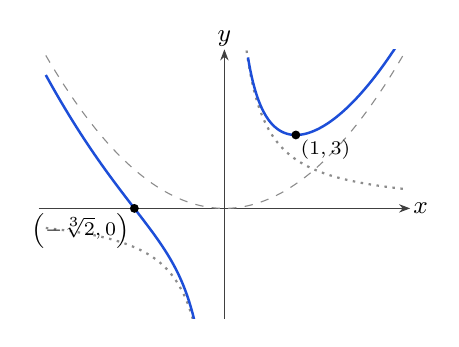
\begin{tikzpicture}
\begin{axis}[mygraph, width=6.3cm, height=5.0cm, xmin=-2.6, xmax=2.6, ymin=-4.5, ymax=6.5, xtick=\empty, ytick=\empty]
  \addplot[black!45, dashed, thin, domain=-2.5:2.5] {x^2};
  \addplot[black!45, dotted, thick, domain=-2.5:-0.31] {2/x};
  \addplot[black!45, dotted, thick, domain=0.31:2.5] {2/x};
  \addplot[plotA, domain=-2.5:-0.36, samples=300] {x^2+2/x};
  \addplot[plotA, domain=0.33:2.5, samples=300] {x^2+2/x};
  \node[pt] at (axis cs:1,3) {}; \node[lab, below right] at (axis cs:1,3) {$(1,3)$};
  \node[pt] at (axis cs:-1.26,0) {}; \node[lab, below left] at (axis cs:-1.26,0) {$\left(-\sqrt[3]{2},0\right)$};
\end{axis}
\end{tikzpicture}

{\scriptsize Dashed: $y=x^2$; dotted: $y=\frac2x$; solid: the sum.}
\end{cols}

% -----------------------------------------------------------------
\subsection{Piecewise (hybrid) functions}
\label{sec:hybrid}

\begin{cols}
\begin{defn}{Hybrid functions}
A hybrid function uses different rules on different parts of its domain, e.g.
\[f(x)=\begin{cases} x^2+1, & x<1\\ 3-x, & x\ge1.\end{cases}\]
\begin{itemize}
  \item Sketch each rule \emph{only} over its own interval; show endpoints as open or closed.
  \item \textbf{Continuous} at a join $x=a$ if both pieces give the same value there (here both give $2$ at $x=1$).
  \item \textbf{Smooth} (differentiable) at the join if the gradients also match. Here the left gradient is $2x=2$ and the right gradient is $-1$, so there is a corner and $f$ is not differentiable at $x=1$ (see \S\ref{sec:cont}).
\end{itemize}
\end{defn}
\nextcol
\centering
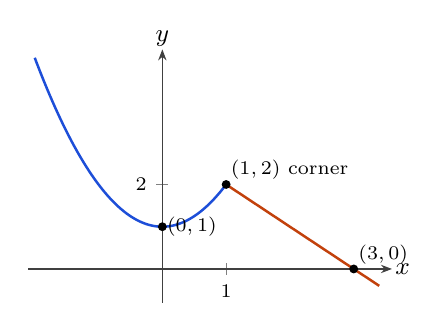
\begin{tikzpicture}
\begin{axis}[mygraph, width=6.2cm, height=4.8cm, xmin=-2.1, xmax=3.6, ymin=-0.8, ymax=5.2, xtick={1}, ytick={2}]
  \addplot[plotA, domain=-2:1] {x^2+1};
  \addplot[plotB, domain=1:3.4] {3-x};
  \node[pt] at (axis cs:1,2) {}; \node[lab, above right] at (axis cs:1,2) {$(1,2)$ corner};
  \node[pt] at (axis cs:0,1) {}; \node[lab, right] at (axis cs:0,1) {$(0,1)$};
  \node[pt] at (axis cs:3,0) {}; \node[lab, above right] at (axis cs:3,0) {$(3,0)$};
\end{axis}
\end{tikzpicture}
\end{cols}

% -----------------------------------------------------------------
\subsection{Modelling with functions}
\label{sec:model}

\begin{keyres}{Recognising a model from a graph or a table}
\begin{center}
\small
\begin{tabularx}{\linewidth}{@{}lL@{}}
\toprule
Feature of the data or graph & Possible model \\
\midrule
Constant rate of change (equal differences in $y$ for equal steps in $x$) & Linear $y=mx+c$ \\
Single maximum or minimum, symmetric & Quadratic $y=a(x-h)^2+k$ \\
Constant \emph{ratio} for equal steps (equal percentage growth or decay) & Exponential $y=Ae^{kt}$ ($k>0$ growth, $k<0$ decay) \\
Rises or falls towards a limiting value (asymptote) & $y=c-Ae^{-kt}$ (e.g.\ heating, learning curves), $y=c+Ae^{-kt}$ (cooling) \\
Fast initial increase that keeps slowing (no asymptote) & $y=a\loge(x)+b$ or $y=ax^n$ with $0<n<1$ \\
Repeating pattern (tides, temperature, daylight) & $y=a\sin(n(t-b))+c$: $c$ = mean, $a$ = (max $-$ min)/2, period $=\frac{2\pi}{n}$ \\
Different behaviour over different intervals & Hybrid function (check continuity at the joins) \\
\bottomrule
\end{tabularx}
\end{center}
\textbf{Finding parameters:} substitute known points (simultaneous equations), use features (max, min, period, asymptote), or use CAS regression. \textbf{In context}, always state a sensible domain (e.g.\ $t\ge0$), include units and comment on whether the model is valid outside the data.
\end{keyres}

\begin{cols}
\begin{example}{circular model}
A day's temperature has a maximum of $28^\circ$C at 3 pm ($t=15$) and a minimum of $12^\circ$C at 3 am ($t=3$). Model $T=A\sin\!\left(\frac{\pi}{12}(t-b)\right)+c$.\par
Mean $c=\frac{28+12}{2}=20$, amplitude $A=\frac{28-12}{2}=8$, period 24 h so $n=\frac{2\pi}{24}=\frac{\pi}{12}$.\par
The maximum occurs when $\frac{\pi}{12}(15-b)=\frac{\pi}{2}$, so $b=9$.\par
$T(t)=8\sin\!\left(\frac{\pi}{12}(t-9)\right)+20$. Check: $T(3)=8\sin\!\left(-\frac{\pi}{2}\right)+20=12$. \tick
\end{example}
\nextcol
\begin{example}{exponential model}
A population is $500$ at $t=0$ and $2000$ at $t=3$. Model $N=Ae^{kt}$.\par
$N(0)=A=500$. \ $500e^{3k}=2000\Rightarrow e^{3k}=4\Rightarrow k=\frac{\loge4}{3}=\frac{2\loge2}{3}$.\par
So $N(t)=500e^{\frac{2\loge2}{3}t}=500\cdot4^{t/3}$.\par
The population doubles every $\frac{\loge2}{k}=1.5$ time units.
\end{example}
\end{cols}

% =================================================================
\section{Algebra, number and structure (Area of Study 2)}
\label{sec:algebra}
% =================================================================

\begin{sdbox}
\textbf{This area of study includes:}
\begin{itemize}
  \item solution of polynomial equations with real coefficients of degree $n$ having up to $n$ real solutions, including numerical solutions
  \item functions and their inverses, including conditions for the existence of an inverse function, and use of inverse functions to solve equations involving exponential, logarithmic, circular and power functions
  \item composition of functions, where $f$ composite $g$, $f\circ g$, is defined by $(f\circ g)(x)=f(g(x))$ given $r_g\subseteq d_f$
  \item solution of equations of the form $f(x)=g(x)$ over a specified interval, by graphical, numerical and algebraic methods, as applicable
  \item solution of literal equations and general solution of equations involving a single parameter
  \item solution of simple systems of simultaneous linear equations, including cases where no solution or an infinite number of solutions exist (geometric interpretation only required for two equations in two variables)
\end{itemize}
\textbf{Key skills:} find the rule, domain and range of inverse and composite functions; apply analytical, graphical and numerical processes (including \textbf{Newton's method}, \S\ref{sec:newton}) to obtain exact or approximate, general or specific solutions and verify them; \byhand\ solve $\sin(ax+b)=c$, $\cos(ax+b)=c$, $\tan(ax+b)=c$ with exact solutions over a given interval; use algebraic, logarithmic and circular function properties to simplify expressions and solve equations. This content is \emph{``incorporated as applicable to the other areas of study''}, so expect it inside calculus and probability questions.
\end{sdbox}

\subsection{Polynomial equations}
\label{sec:polyeq}

\begin{keyres}{Theorems and techniques}
\begin{itemize}
  \item A polynomial equation of degree $n$ (real coefficients) has \textbf{at most $n$ real solutions}.
  \item \textbf{Remainder theorem:} the remainder when $P(x)$ is divided by $(x-a)$ is $P(a)$; for $(ax-b)$ it is $P\!\left(\frac ba\right)$.
  \item \textbf{Factor theorem:} $(x-a)$ is a factor of $P(x)\iff P(a)=0$.
  \item \textbf{Rational root test:} any rational root of $a_nx^n+\dots+a_0$ is $\pm\dfrac{\text{factor of }a_0}{\text{factor of }a_n}$. Try $\pm1,\pm2,\dots$ first.
  \item Divide by long division or by \textbf{equating coefficients}; factorise the quotient.
  \item \textbf{Substitution} for ``quadratic-type'' equations: $u=x^2$, $u=e^x$, $u=2^x$, $u=\sin x$, $u=\sqrt{x}$.
  \item No exact method? Solve \textbf{numerically}: CAS, graph intersections, Newton's method (\S\ref{sec:newton}) or bisection (\S\ref{sec:algorithms}).
\end{itemize}
\end{keyres}

\begin{cols}
\begin{example}{a cubic by the factor theorem \byhand}
Solve $x^3-4x^2+x+6=0$.\par
Try $x=-1$: $-1-4-1+6=0$, so $(x+1)$ is a factor.\par
Equate coefficients: $x^3-4x^2+x+6=(x+1)(x^2+bx+c)$ gives $c=6$, $b+1=-4\Rightarrow b=-5$.\par
$(x+1)(x^2-5x+6)=(x+1)(x-2)(x-3)=0$, so $x=-1,2,3$.
\end{example}
\nextcol
\begin{example}{unknown coefficient \byhand}
$(x-2)$ is a factor of $P(x)=x^3+kx^2-4x+12$. Find $k$ and solve $P(x)=0$.\par
$P(2)=8+4k-8+12=0\Rightarrow k=-3$.\par
$P(x)=x^3-3x^2-4x+12=x^2(x-3)-4(x-3)$\\ $=(x-3)(x-2)(x+2)$, so $x=-2,2,3$.
\end{example}
\end{cols}

\begin{example}{substitution and the discriminant \byhand}
\textbf{(a)} $x^4-5x^2+4=0$: let $u=x^2$. Then $u^2-5u+4=(u-1)(u-4)=0$, so $x^2=1$ or $4$, giving $x=\pm1,\pm2$.\par
\textbf{(b)} $2^{2x}-3\cdot2^x-4=0$: let $u=2^x$. Then $(u-4)(u+1)=0$; $2^x=-1$ is impossible, so $2^x=4$ and $x=2$.\par
\textbf{(c)} For which $m$ does the line $y=mx-1$ meet the parabola $y=x^2+3$? Equating gives $x^2-mx+4=0$, with $\Delta=m^2-16$. There are two intersections if $|m|>4$, the line is a \textbf{tangent} if $m=\pm4$, and there are no intersections if $-4<m<4$.
\end{example}

% -----------------------------------------------------------------
\subsection{Inverse functions}
\label{sec:inverse}

\begin{keyres}{Inverse functions}
\begin{itemize}
  \item $f^{-1}$ exists \textbf{if and only if $f$ is one-to-one} (horizontal line test). Many-to-one functions need a \emph{restricted domain} first.
  \item \boldmath$d_{f^{-1}}=r_f$ \textbf{and} $r_{f^{-1}}=d_f$.\unboldmath
  \item $f\!\left(f^{-1}(x)\right)=x$ for $x\in d_{f^{-1}}$, and $f^{-1}(f(x))=x$ for $x\in d_f$.
  \item The graph of $y=f^{-1}(x)$ is the \textbf{reflection of $y=f(x)$ in the line $y=x$}: $(a,b)\to(b,a)$, and asymptote $x=h\leftrightarrow y=h$.
  \item Inverse pairs: $e^x\leftrightarrow\loge x$; \ $a^x\leftrightarrow\log_ax$; \ $x^2\ (x\ge0)\leftrightarrow\sqrt{x}$; \ $x^3\leftrightarrow\sqrt[3]{x}$; \ $\frac1x$ is its own inverse.
  \item Circular functions are many-to-one, but CAS uses $\sin^{-1}$, $\cos^{-1}$, $\tan^{-1}$ (principal values in $\left[-\frac\pi2,\frac\pi2\right]$, $[0,\pi]$, $\left(-\frac\pi2,\frac\pi2\right)$) to solve equations; you then find the other solutions by symmetry.
\end{itemize}
\end{keyres}

\begin{method}{Finding $f^{-1}$}
\begin{enumerate}
  \item State the domain and range of $f$, and check $f$ is one-to-one.
  \item Swap $x$ and $y$: \ $x=f(y)$.
  \item Solve for $y$. If there is a $\pm$, choose the sign that matches $r_{f^{-1}}=d_f$.
  \item Write the answer in full: $f^{-1}:r_f\to\R,\ f^{-1}(x)=\dots$
\end{enumerate}
\end{method}

\begin{example}{finding inverse functions \byhand}
\begin{tabularx}{\linewidth}{@{}p{4.4cm}L@{}}
$f:[1,\infty)\to\R,\ f(x)=(x-1)^2+2$ & $r_f=[2,\infty)$. Swap: $x=(y-1)^2+2\Rightarrow y=1\pm\sqrt{x-2}$. We need $y\ge1$, so take $+$:\par $f^{-1}:[2,\infty)\to\R,\ f^{-1}(x)=1+\sqrt{x-2}$. \\[3pt]
$g:\R\to\R,\ g(x)=3e^{2x}-1$ & $r_g=(-1,\infty)$. Swap: $x=3e^{2y}-1\Rightarrow e^{2y}=\frac{x+1}{3}$:\par $g^{-1}:(-1,\infty)\to\R,\ g^{-1}(x)=\frac12\loge\!\left(\frac{x+1}{3}\right)$. \\[3pt]
$h:(2,\infty)\to\R,\ h(x)=\loge(x-2)+1$ & $r_h=\R$. Swap: $x=\loge(y-2)+1\Rightarrow y=e^{x-1}+2$:\par $h^{-1}:\R\to\R,\ h^{-1}(x)=e^{x-1}+2$. \\
\end{tabularx}
\end{example}

\begin{cols}
\begin{keyres}{Restricting the domain; intersections with the inverse}
\begin{itemize}
  \item \textbf{Largest domain for an inverse:} cut the graph at turning points. E.g.\ $f(x)=x^2-4x+1=(x-2)^2-3$ is one-to-one on $[2,\infty)$ or $(-\infty,2]$.
  \item If $f$ is \textbf{strictly increasing}, every intersection of $y=f(x)$ and $y=f^{-1}(x)$ lies on $y=x$, so solve the easier equation $f(x)=x$.
  \item If $f$ is \textbf{decreasing}, there can be intersections \emph{off} the line $y=x$. Solve $f(x)=f^{-1}(x)$ (or use CAS). Example: $f(x)=-x^3$, $f^{-1}(x)=-\sqrt[3]{x}$ meet at $(0,0)$, $(1,-1)$ and $(-1,1)$. Only $(0,0)$ is on $y=x$.
\end{itemize}
\end{keyres}
\nextcol
\centering
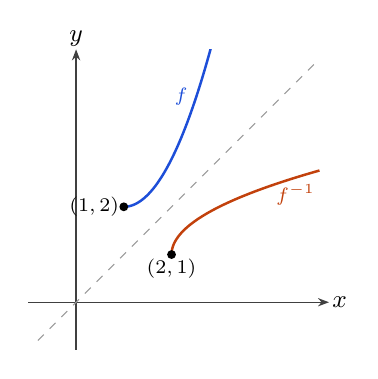
\begin{tikzpicture}
\begin{axis}[mygraph, width=5.4cm, height=5.4cm, xmin=-1.0, xmax=5.3, ymin=-1.0, ymax=5.3, xtick=\empty, ytick=\empty]
  \addplot[black!40, dashed, thin, domain=-0.8:5.1] {x};
  \addplot[plotA, domain=1:2.95] {(x-1)^2+2};
  \addplot[plotB, domain=2:5.1, samples=300] {1+sqrt(x-2)};
  \node[pt] at (axis cs:1,2) {}; \node[lab, left] at (axis cs:1,2) {$(1,2)$};
  \node[pt] at (axis cs:2,1) {}; \node[lab, below] at (axis cs:2,1) {$(2,1)$};
  \node[lab, plotA] at (axis cs:2.2,4.3) {$f$};
  \node[lab, plotB] at (axis cs:4.6,2.25) {$f^{-1}$};
\end{axis}
\end{tikzpicture}\hfill
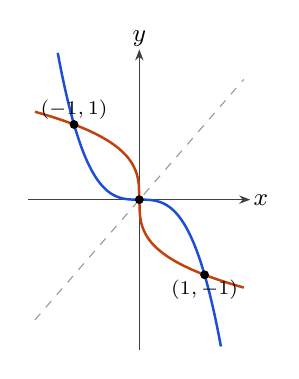
\begin{tikzpicture}
\begin{axis}[mygraph, width=4.4cm, height=5.4cm, xmin=-1.7, xmax=1.7, ymin=-2.0, ymax=2.0, xtick=\empty, ytick=\empty]
  \addplot[black!40, dashed, thin, domain=-1.6:1.6] {x};
  \addplot[plotA, domain=-1.25:1.25] {-x^3};
  \addplot[plotB, domain=-1.6:1.6] {-sign(x)*abs(x)^(1/3)};
  \node[pt] at (axis cs:1,-1) {}; \node[lab, below] at (axis cs:1,-1) {$(1,-1)$};
  \node[pt] at (axis cs:-1,1) {}; \node[lab, above] at (axis cs:-1,1) {$(-1,1)$};
  \node[pt] at (axis cs:0,0) {};
\end{axis}
\end{tikzpicture}

{\scriptsize Left: $f(x)=(x-1)^2+2$, $x\ge1$, and its inverse (no intersection). Right: $y=-x^3$ and its inverse meet off the line $y=x$.}
\end{cols}

% -----------------------------------------------------------------
\subsection{Composite functions}
\label{sec:composite}

\begin{keyres}{Composite functions $f\circ g$}
\begin{itemize}
  \item $(f\circ g)(x)=f(g(x))$: apply $g$ first, then $f$.
  \item \textbf{Exists if and only if} $r_g\subseteq d_f$ (the outputs of $g$ must be allowed inputs of $f$).
  \item Then \boldmath$d_{f\circ g}=d_g$\unboldmath. This is the domain of the \emph{inner} function, \emph{not} the implied domain of the simplified rule.
  \item \textbf{Range:} find the set of values $f$ takes when its inputs are restricted to $r_g$.
  \item If $r_g\not\subseteq d_f$, restrict the domain of $g$ until its range fits inside $d_f$.
  \item In general $f\circ g\ne g\circ f$. Note $f^{-1}\circ f$ is the identity on $d_f$.
\end{itemize}
\end{keyres}

\begin{example}{composite functions \byhand}
Let $f:[0,\infty)\to\R,\ f(x)=\sqrt{x}$ and $g:\R\to\R,\ g(x)=1-x^2$.\par
\textbf{$f\circ g$:} $r_g=(-\infty,1]\not\subseteq[0,\infty)=d_f$, so $f\circ g$ \emph{does not exist} with $d_g=\R$. Restrict $g$ to $[-1,1]$: then $r_g=[0,1]\subseteq d_f$ \tick. \ $(f\circ g)(x)=\sqrt{1-x^2}$, domain $[-1,1]$, range $[0,1]$.\par
\textbf{$g\circ f$:} $r_f=[0,\infty)\subseteq\R=d_g$ \tick. \ $(g\circ f)(x)=1-(\sqrt{x})^2=1-x$ with \textbf{domain $[0,\infty)$} (the domain of $f$), so range $(-\infty,1]$.\par
\textbf{Maximal domain question:} for $f(x)=\loge(x)$ and $g(x)=4-x^2$, $f\circ g$ needs $4-x^2>0$, so the largest domain of $g$ is $(-2,2)$.
\end{example}

% -----------------------------------------------------------------
\subsection{Solving equations $f(x)=g(x)$: exact, graphical and numerical}
\label{sec:solve}

\begin{method}{General approach}
\begin{enumerate}
  \item Note any domain restrictions (logs: argument $>0$; roots; denominators; the given interval).
  \item Choose a method: \textbf{algebraic/exact} (factorise, inverse operations, log/index laws, substitution); \textbf{graphical} (intersections of $y=f(x)$ and $y=g(x)$, which also shows the \emph{number} of solutions); \textbf{numerical} (CAS solve, Newton's method, bisection) when no exact method exists.
  \item \textbf{Check} every solution satisfies the original equation and the domain. Reject extraneous solutions, and say why.
\end{enumerate}
\end{method}

\begin{example}{exponential, logarithmic and power equations \byhand}
\begin{tabularx}{\linewidth}{@{}p{5.1cm}L@{}}
$e^{2x}-5e^x+6=0$ & $(e^x-2)(e^x-3)=0\Rightarrow x=\loge2$ or $\loge3$. \\
$3e^{2x}=7$ & $e^{2x}=\frac73\Rightarrow x=\frac12\loge\!\left(\frac73\right)$. \\
$2^{x+1}=5$ & $x+1=\log_25\Rightarrow x=\log_25-1=\frac{\loge5}{\loge2}-1$. \\
$\loge(2x-1)=3$ & $2x-1=e^3\Rightarrow x=\frac{e^3+1}{2}$. \\
$\loge x+\loge(x-3)=\loge4$ & Need $x>3$. $\loge(x(x-3))=\loge4\Rightarrow x^2-3x-4=0\Rightarrow(x-4)(x+1)=0$. Reject $x=-1$, so $x=4$. \\
$\log_{10}x+\log_{10}(x-21)=2$ & Need $x>21$. $x(x-21)=100\Rightarrow(x-25)(x+4)=0\Rightarrow x=25$. \\
$\log_2x-\log_2(x-1)=3$ & $\frac{x}{x-1}=2^3=8\Rightarrow x=8x-8\Rightarrow x=\frac87$ (valid since $x>1$). \\
$x^{3/2}=8$; \quad $2x^{-1/2}=6$ & $x=8^{2/3}=4$; \quad $x^{-1/2}=3\Rightarrow x=\frac19$. \\
\end{tabularx}
\end{example}

\subsection{Circular equations}
\label{sec:circeq}

\begin{method}{Solving $\sin(ax+b)=c$, $\cos(ax+b)=c$, $\tan(ax+b)=c$ over an interval \byhand}
\begin{enumerate}
  \item Isolate the circular function and let $\theta=ax+b$.
  \item \textbf{Change the interval:} if $x\in[p,q]$ and $a>0$, then $\theta\in[ap+b,\ aq+b]$.
  \item Find the \textbf{base angle} from $|c|$ using exact values (e.g.\ $|c|=\frac{\sqrt3}{2}\Rightarrow\frac{\pi}{3}$ for $\sin$).
  \item Use the sign of $c$ and ASTC to find the quadrants, list all $\theta$ in the new interval by adding $2\pi$ (sin, cos) or $\pi$ (tan) repeatedly, then solve for $x$.
\end{enumerate}
\end{method}

\begin{example}{circular equations \byhand}
\textbf{(a)} $2\sin(3x)=\sqrt3$, $x\in[0,\pi]$. Then $\sin(3x)=\frac{\sqrt3}{2}$ with $3x\in[0,3\pi]$, so $3x=\frac{\pi}{3},\frac{2\pi}{3},\frac{7\pi}{3},\frac{8\pi}{3}$ and $x=\frac{\pi}{9},\frac{2\pi}{9},\frac{7\pi}{9},\frac{8\pi}{9}$.\par
\textbf{(b)} $\cos\!\left(2x+\frac{\pi}{3}\right)=-\frac12$, $x\in[0,\pi]$. Here $2x+\frac{\pi}{3}\in\left[\frac{\pi}{3},\frac{7\pi}{3}\right]$, and cos is negative in quadrants 2 and 3: $2x+\frac{\pi}{3}=\frac{2\pi}{3},\frac{4\pi}{3}$, so $x=\frac{\pi}{6},\frac{\pi}{2}$.\par
\textbf{(c)} $\tan\!\left(\frac x2\right)=-1$, $x\in[0,4\pi]$. Here $\frac x2\in[0,2\pi]$: $\frac x2=\frac{3\pi}{4},\frac{7\pi}{4}$, so $x=\frac{3\pi}{2},\frac{7\pi}{2}$.\par
\textbf{(d)} $\sin x=\sqrt3\cos x$, $x\in[0,2\pi]$. Divide by $\cos x$ (allowed: $\cos x=0$ gives no solutions): $\tan x=\sqrt3$, so $x=\frac{\pi}{3},\frac{4\pi}{3}$.\par
\textbf{(e)} $2\sin^2x-\sin x-1=0$, $x\in[0,2\pi]$. Factorise: $(2\sin x+1)(\sin x-1)=0$. $\sin x=1\Rightarrow x=\frac{\pi}{2}$; \ $\sin x=-\frac12\Rightarrow x=\frac{7\pi}{6},\frac{11\pi}{6}$.
\end{example}

\begin{cols}
\begin{keyres}{General solutions ($k\in\Z$)}
\begin{itemize}
  \item $\sin\theta=c$: $\theta=\sin^{-1}(c)+2k\pi$ or $\theta=\pi-\sin^{-1}(c)+2k\pi$
  \item $\cos\theta=c$: $\theta=\pm\cos^{-1}(c)+2k\pi$
  \item $\tan\theta=c$: $\theta=\tan^{-1}(c)+k\pi$
\end{itemize}
\textbf{Examples:} $\sin(2x)=\frac12\Rightarrow x=\frac{\pi}{12}+k\pi$ or $x=\frac{5\pi}{12}+k\pi$. \ $\tan(3x)=1\Rightarrow x=\frac{\pi}{12}+\frac{k\pi}{3}$. \ $\cos x=\frac{\sqrt2}{2}\Rightarrow x=\pm\frac{\pi}{4}+2k\pi$.
\end{keyres}
\nextcol
\begin{tip}[Counting solutions and non-exact values]
\begin{itemize}
  \item $\sin(nx)=c$ with $-1<c<1$, $c\ne0$, has $2n$ solutions in $[0,2\pi]$ (two per cycle, and there are $n$ cycles). Check the endpoints separately when $c=0$ or $c=\pm1$.
  \item Non-exact: $\sin x=0.3$, $x\in[0,2\pi]$ gives $x=\sin^{-1}(0.3)\approx0.3047$ or $\pi-0.3047\approx2.8369$.
  \item CAS gives general solutions with an arbitrary integer (e.g.\ \texttt{n1} or \texttt{constn}). Rewrite it as $k\in\Z$.
\end{itemize}
\end{tip}
\end{cols}

% -----------------------------------------------------------------
\subsection{Literal equations and equations with a parameter}
\label{sec:literal}

\begin{cols}
\begin{keyres}{Literal equations}
A literal equation has letters (parameters) as well as the unknown. Solve for the unknown in terms of the others, \textbf{stating restrictions}.
\begin{itemize}
  \item $V=\frac43\pi r^3\Rightarrow r=\sqrt[3]{\dfrac{3V}{4\pi}}$.
  \item $y=\dfrac{ax+b}{cx+d}\Rightarrow ycx+yd=ax+b\Rightarrow x=\dfrac{b-dy}{cy-a}$, \ $cy\ne a$.
  \item $e^{kx}=5\Rightarrow x=\dfrac{\loge5}{k}$, \ $k\ne0$.
\end{itemize}
\end{keyres}
\nextcol
\begin{example}{a single parameter}
\textbf{(a)} Solve $kx-3=2x+k$ for $x$: $x(k-2)=k+3\Rightarrow x=\frac{k+3}{k-2}$ for $k\ne2$. If $k=2$ the equation is $-3=2$, so there is no solution.\par
\textbf{(b)} Number of solutions of $kx^2+4x+k=0$. If $k=0$: $4x=0$, one solution (not a quadratic!). If $k\ne0$: $\Delta=16-4k^2$. Two solutions for $-2<k<2$, $k\ne0$; one for $k=\pm2$; none for $|k|>2$.\par
\textbf{(c)} $x^3-3x=k$ has three solutions when $-2<k<2$: the graph of $y=x^3-3x$ has a local max at $(-1,2)$ and a local min at $(1,-2)$. Two solutions if $k=\pm2$, one if $|k|>2$.
\end{example}
\end{cols}

% -----------------------------------------------------------------
\subsection{Simultaneous linear equations}
\label{sec:simul}

\begin{keyres}{Two equations, two unknowns: $a_1x+b_1y=c_1$, \ $a_2x+b_2y=c_2$}
\begin{center}
\small
\begin{tabularx}{\linewidth}{@{}lLL@{}}
\toprule
Number of solutions & Geometry (two lines) & Algebraic condition \\
\midrule
Unique solution & Lines intersect at one point (different gradients) & $a_1b_2-a_2b_1\ne0$ \\
No solution & Parallel, distinct lines (same gradient, different intercepts) & $a_1b_2-a_2b_1=0$ and the equations are inconsistent \\
Infinitely many & Same line (one equation is a multiple of the other) & $a_1b_2-a_2b_1=0$ and the equations are consistent \\
\bottomrule
\end{tabularx}
\end{center}
$a_1b_2-a_2b_1$ is the determinant of the coefficient matrix (CAS: \texttt{det}). Comparing gradients and $y$-intercepts always works too. For \textbf{three equations in three unknowns}, use elimination or CAS. There can again be one, none or infinitely many solutions (no geometric interpretation needed).
\end{keyres}

\begin{example}{systems with a parameter}
For which $k$ does the system $kx+3y=6$, \ $4x+(k+4)y=k+10$ have (a) a unique solution, (b) no solution, (c) infinitely many solutions?\par
\textbf{Determinant:} $k(k+4)-3\times4=k^2+4k-12=(k+6)(k-2)$.\par
\textbf{(a)} Unique solution for $k\in\R\setminus\{-6,2\}$. It is $x=\frac{3}{k+6}$, $y=\frac{k+12}{k+6}$.\par
\textbf{(b), (c)} Test the two remaining values:
\begin{itemize}
  \item $k=2$: $2x+3y=6$ and $4x+6y=12$. The second is twice the first, so it is the same line and there are \textbf{infinitely many} solutions: $\left(3-\frac{3t}{2},\,t\right)$, $t\in\R$.
  \item $k=-6$: $-6x+3y=6\iff y=2x+2$ and $4x-2y=4\iff y=2x-2$. Parallel, distinct lines, so \textbf{no solution}.
\end{itemize}
\textbf{Three unknowns:} $x+y+z=6$, \ $2x-y+z=3$, \ $x+2y-z=2$ has the unique solution $(1,2,3)$ (check by substitution).
\end{example}

% -----------------------------------------------------------------
\subsection{Properties of functions (functional equations)}
\label{sec:funceq}

\begin{tip}[\mcq{} Testing a property]
Questions like ``Which function satisfies $f(x+y)=f(x)f(y)$?'' are tested by substitution, or by trying simple numbers to eliminate options.
\begin{itemize}
  \item $f(x+y)=f(x)f(y)$: \ $f(x)=e^{kx}$ (since $e^{k(x+y)}=e^{kx}e^{ky}$) or $a^x$.
  \item $f(xy)=f(x)+f(y)$: \ $f(x)=\log_a(x)$. \qquad $f(x+y)=f(x)+f(y)$: \ $f(x)=kx$.
  \item $f(-x)=f(x)$: even. \ $f(-x)=-f(x)$: odd. \ $f(f(x))=x$: self-inverse (e.g.\ $\frac1x$, $-x$, $a-x$).
  \item To \emph{disprove} a property, one counter-example is enough (e.g.\ $x=y=1$).
\end{itemize}
\end{tip}

% =================================================================
\section{Calculus I: differentiation and its applications (Area of Study 3)}
\label{sec:diff}
% =================================================================

\begin{sdbox}
\textbf{Calculus covers} \emph{``graphical treatment of limits, continuity and differentiability of functions of a single real variable, and differentiation, anti-differentiation and integration of these functions''}. The differentiation dot points are:
\begin{itemize}
  \item deducing the graph of the derivative function from the graph of a given function
  \item derivatives of $x^n$ for $n\in\Q$, $e^x$, $\loge(x)$, $\sin(x)$, $\cos(x)$ and $\tan(x)$
  \item derivatives of $f(x)\pm g(x)$, $f(x)\times g(x)$, $\dfrac{f(x)}{g(x)}$ and $(f\circ g)(x)$, where $f$ and $g$ are polynomial, exponential, circular, logarithmic or power functions and transformations or simple combinations of these
  \item application of differentiation to graph sketching and identification of key features, including stationary points and points of inflection, and intervals over which a function is strictly increasing or strictly decreasing
  \item identification of local maximum/minimum values over an interval and application to solving optimisation problems in context, including identification of interval endpoint maximum and minimum values
\end{itemize}
\textbf{Key knowledge/skills:} the link between the graph of a function and its gradient function; the tangent at a point; how the sign and magnitude of $f'$ describe $f$; the sum, difference, chain, product and quotient rules (\byhand\ for simple combinations); derivatives of $f(ax+b)$ for $f=x^n,\sin,\cos,\tan,e^x,\loge x$ \byhand; \textbf{Newton's method}.
\end{sdbox}

\subsection{Limits, continuity and differentiability}
\label{sec:cont}

\begin{defn}{Definitions (graphical treatment)}
\begin{itemize}
  \item $\displaystyle\lim_{x\to a}f(x)=L$: $f(x)$ gets arbitrarily close to $L$ as $x$ approaches $a$ from both sides. The left limit $\lim_{x\to a^-}$ and right limit $\lim_{x\to a^+}$ must be equal. Limits at infinity describe asymptotes, e.g.\ $\lim_{x\to\infty}e^{-x}=0$.
  \item $f$ is \textbf{continuous at $x=a$} if $f(a)$ is defined, $\lim_{x\to a}f(x)$ exists, and they are equal. Informally, you can draw through $x=a$ without lifting your pen.
  \item $f$ is \textbf{differentiable at $x=a$} if $f'(a)=\lim_{h\to0}\dfrac{f(a+h)-f(a)}{h}$ exists: the graph is \emph{smooth} there (left and right gradients equal and finite).
  \item Differentiable $\Rightarrow$ continuous, but \textbf{continuous $\not\Rightarrow$ differentiable}.
  \item \textbf{Not differentiable} at: corners (e.g.\ at hybrid joins), cusps ($x^{2/3}$ at $0$), vertical tangents ($x^{1/3}$ at $0$), any discontinuity, and the \textbf{endpoints} of a closed domain. The domain of $f'$ excludes all of these, so $f'$ is defined on open intervals.
\end{itemize}
\end{defn}

\begin{center}
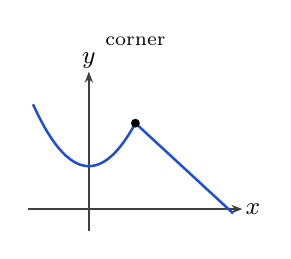
\begin{tikzpicture}
\begin{axis}[smallgraph, width=4.3cm, height=3.6cm, title={\scriptsize corner}, xmin=-1.3, xmax=3.3, ymin=-0.5, ymax=3.2, xtick=\empty, ytick=\empty]
  \addplot[plotA, domain=-1.2:1] {x^2+1};
  \addplot[plotA, domain=1:3.1] {3-x};
  \node[pt] at (axis cs:1,2) {};
\end{axis}
\end{tikzpicture}\hfill
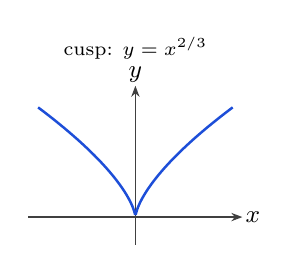
\begin{tikzpicture}
\begin{axis}[smallgraph, width=4.3cm, height=3.6cm, title={\scriptsize cusp: $y=x^{2/3}$}, xmin=-2.2, xmax=2.2, ymin=-0.4, ymax=1.9, xtick=\empty, ytick=\empty]
  \addplot[plotA, domain=-2:2] {abs(x)^(2/3)};
\end{axis}
\end{tikzpicture}\hfill
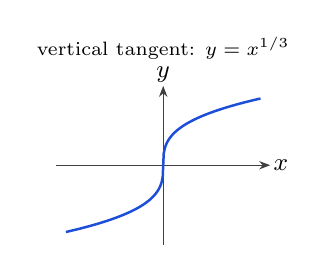
\begin{tikzpicture}
\begin{axis}[smallgraph, width=4.3cm, height=3.6cm, title={\scriptsize vertical tangent: $y=x^{1/3}$}, xmin=-2.2, xmax=2.2, ymin=-1.5, ymax=1.5, xtick=\empty, ytick=\empty]
  \addplot[plotA, domain=-2:2] {sign(x)*abs(x)^(1/3)};
\end{axis}
\end{tikzpicture}\hfill
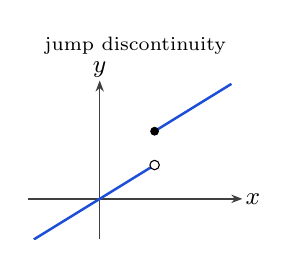
\begin{tikzpicture}
\begin{axis}[smallgraph, width=4.3cm, height=3.6cm, title={\scriptsize jump discontinuity}, xmin=-1.3, xmax=2.6, ymin=-1.2, ymax=3.5, xtick=\empty, ytick=\empty]
  \addplot[plotA, domain=-1.2:1] {x};
  \addplot[plotA, domain=1:2.4] {x+1};
  \node[opt] at (axis cs:1,1) {};
  \node[pt] at (axis cs:1,2) {};
\end{axis}
\end{tikzpicture}
\end{center}

\begin{example}{making a hybrid function smooth}
Find $a$ and $b$ so that $f(x)=\begin{cases}ax^2+b, & x\le1\\ 4\sqrt{x}, & x>1\end{cases}$ is differentiable at $x=1$.\par
\textbf{Continuity:} $a(1)^2+b=4\sqrt1\Rightarrow a+b=4$.\quad
\textbf{Equal gradients:} left $2ax\big|_{x=1}=2a$; right $\ddx\left(4x^{1/2}\right)=2x^{-1/2}\big|_{x=1}=2$. So $2a=2$, giving $a=1$ and $b=3$.
\end{example}

\begin{keyres}{Rates of change and first principles (assumed from Units 1 \& 2)}
\begin{itemize}
  \item \textbf{Average rate of change} of $f$ over $[a,b]$: $\dfrac{f(b)-f(a)}{b-a}$, the gradient of the chord (secant).
  \item \textbf{Instantaneous rate of change} at $x=a$: $f'(a)$, the gradient of the tangent.
  \item First principles: $f'(x)=\displaystyle\lim_{h\to0}\frac{f(x+h)-f(x)}{h}$. E.g.\ for $f(x)=x^2$: $\dfrac{(x+h)^2-x^2}{h}=2x+h\to2x$.
\end{itemize}
\end{keyres}

% -----------------------------------------------------------------
\subsection{Standard derivatives and the rules}
\label{sec:rules}

\begin{cols}[0.47]
\begin{keyres}{Standard derivatives}
\renewcommand{\arraystretch}{1.45}
\begin{tabular}{@{}l@{\quad}l@{}}
$f(x)$ & $f'(x)$ \\ \hline
$x^n$, $n\in\Q$ & $nx^{n-1}$ \\
$(ax+b)^n$ & $an(ax+b)^{n-1}$ \\
$e^{x}$ & $e^{x}$ \\
$e^{ax+b}$ & $ae^{ax+b}$ \\
$\loge(x)$, $x>0$ & $\dfrac1x$ \\
$\loge(ax+b)$ & $\dfrac{a}{ax+b}$ \\
$\sin(ax+b)$ & $a\cos(ax+b)$ \\
$\cos(ax+b)$ & $-a\sin(ax+b)$ \\
$\tan(ax+b)$ & $\dfrac{a}{\cos^2(ax+b)}=a\sec^2(ax+b)$ \\
$a^x=e^{x\loge a}$ & $(\loge a)\,a^x$ \\
\end{tabular}
\par\smallskip
{\small Note: $\ddx\loge(kx)=\dfrac1x$, since $\loge(kx)=\loge k+\loge x$.}
\end{keyres}
\nextcol[0.505]
\begin{keyres}{The rules (with $u=u(x)$, $v=v(x)$)}
\begin{itemize}
  \item Sum/difference: $(f\pm g)'=f'\pm g'$; \ constant multiple $(kf)'=kf'$.
  \item \textbf{Product rule:} $\dfrac{d}{dx}(uv)=u\dfrac{dv}{dx}+v\dfrac{du}{dx}$
  \item \textbf{Quotient rule:} $\dfrac{d}{dx}\!\left(\dfrac uv\right)=\dfrac{v\frac{du}{dx}-u\frac{dv}{dx}}{v^2}$
  \item \textbf{Chain rule:} $\dfrac{dy}{dx}=\dfrac{dy}{du}\cdot\dfrac{du}{dx}$, i.e.\ $\big(f(g(x))\big)'=f'(g(x))\,g'(x)$
\end{itemize}
\textbf{Chain rule patterns} (learn these):
\begin{itemize}
  \item $\ddx[f(x)]^n=n\,f'(x)\,[f(x)]^{n-1}$
  \item $\ddx e^{f(x)}=f'(x)\,e^{f(x)}$
  \item $\ddx\loge(f(x))=\dfrac{f'(x)}{f(x)}$
  \item $\ddx\sin(f(x))=f'(x)\cos(f(x))$
  \item $\ddx\cos(f(x))=-f'(x)\sin(f(x))$
  \item $\ddx\tan(f(x))=\dfrac{f'(x)}{\cos^2(f(x))}$
\end{itemize}
\end{keyres}
\end{cols}

\begin{example}{differentiation \byhand\ (typical Exam 1)}
\renewcommand{\arraystretch}{1.95}
\begin{tabularx}{\linewidth}{@{}>{$}l<{$}L@{}}
y=(2x-1)^5 & $\dydx=5(2x-1)^4\times2=10(2x-1)^4$ \hfill (chain) \\
y=\sqrt{3x^2+1}=(3x^2+1)^{1/2} & $\dydx=\frac12(3x^2+1)^{-1/2}\times6x=\dfrac{3x}{\sqrt{3x^2+1}}$ \hfill (chain) \\
y=x^2e^{3x} & $\dydx=2x\,e^{3x}+x^2\cdot3e^{3x}=xe^{3x}(3x+2)$ \hfill (product) \\
y=\dfrac{\loge x}{x} & $\dydx=\dfrac{x\cdot\frac1x-\loge x\cdot1}{x^2}=\dfrac{1-\loge x}{x^2}$ \hfill (quotient) \\
y=\dfrac{x}{x^2+1} & $\dydx=\dfrac{(x^2+1)-x(2x)}{(x^2+1)^2}=\dfrac{1-x^2}{(x^2+1)^2}$ \hfill (quotient) \\
y=\cos(x^2) & $\dydx=-2x\sin(x^2)$ \hfill (chain) \\
y=\loge(\cos x) & $\dydx=\dfrac{-\sin x}{\cos x}=-\tan x$ \hfill (chain, log pattern) \\
y=e^{\sin x} & $\dydx=\cos x\,e^{\sin x}$ \hfill (chain) \\
y=\tan(2x) & $\dydx=\dfrac{2}{\cos^2(2x)}$ \\
f(x)=x\sin(2x) & $f'(x)=\sin(2x)+2x\cos(2x)$, so $f'\!\left(\frac{\pi}{4}\right)=\sin\frac{\pi}{2}+\frac{\pi}{2}\cos\frac{\pi}{2}=1$ \\
\end{tabularx}
\end{example}

\begin{tip}[Make differentiation easier]
\begin{itemize}
  \item Rewrite roots and fractions as powers first: $\dfrac{3}{\sqrt x}=3x^{-1/2}$, \ $\dfrac{2}{(1-x)^3}=2(1-x)^{-3}$.
  \item Simplify logs first: $\loge\!\left(\dfrac{x^2}{\sqrt{x+1}}\right)=2\loge|x|-\frac12\loge(x+1)$, so the derivative is $\dfrac2x-\dfrac{1}{2(x+1)}$. (Write $\loge|x|$, or state $x>0$: $\loge(x^2)$ is defined for $x<0$ but $2\loge x$ is not.)
  \item Factorise the answer (e.g.\ $xe^{3x}(3x+2)$). You will usually need $f'(x)=0$ next, and the factor form makes that easy.
  \item ``Show that $f'(x)=\dots$'': show the rule you used and at least one intermediate line.
\end{itemize}
\end{tip}

% -----------------------------------------------------------------
\subsection{Tangents and normals}
\label{sec:tangent}

\begin{cols}
\begin{keyres}{Equations}
At the point $(a,f(a))$:
\begin{itemize}
  \item \textbf{Tangent:} $y-f(a)=f'(a)(x-a)$.
  \item \textbf{Normal} (perpendicular to the tangent): $y-f(a)=-\dfrac{1}{f'(a)}(x-a)$ if $f'(a)\ne0$; if $f'(a)=0$ the normal is the vertical line $x=a$.
  \item Angle of the tangent with the positive $x$-axis: $\tan\theta=f'(a)$.
  \item ``Parallel to $y=mx+c$'': solve $f'(x)=m$.
  \item Linear approximation: $f(a+h)\approx f(a)+hf'(a)$ (the tangent line near $x=a$).
\end{itemize}
\end{keyres}
\nextcol
\begin{example}{tangent, normal, external point \byhand}
\textbf{(a)} $y=x^3-2x$ at $x=1$: $y=-1$, $\dydx=3x^2-2=1$.\\ Tangent $y=x-2$; normal $y=-x$.\par
\textbf{(b)} Tangents to $y=x^2$ that pass through $(1,-3)$. The tangent at $(a,a^2)$ is $y=2ax-a^2$. Substitute $(1,-3)$: $-3=2a-a^2\Rightarrow a^2-2a-3=0\Rightarrow a=3$ or $a=-1$. The tangents are $y=6x-9$ and $y=-2x-1$.
\end{example}
\end{cols}

% -----------------------------------------------------------------
\subsection{The graph of $f'$ from the graph of $f$}
\label{sec:gradgraph}

\begin{cols}[0.53]
\begin{keyres}{Reading the gradient}
\small
\begin{tabular}{@{}p{3.75cm}p{4.45cm}@{}}
\textbf{On the graph of $f$} & \textbf{On the graph of $f'$} \\ \hline
stationary point & $x$-intercept \\
$f$ increasing & above the $x$-axis ($f'>0$) \\
$f$ decreasing & below the $x$-axis ($f'<0$) \\
point of inflection & turning point of $f'$ \\
stationary inflection & touches the $x$-axis \\
steeper & larger $|f'(x)|$ \\
vertical asymptote $x=a$ & vertical asymptote $x=a$ (usually) \\
horizontal asymptote $y=c$ & $f'\to0$ (asymptote $y=0$) \\
polynomial of degree $n$ & polynomial of degree $n-1$ \\
corner, cusp, endpoint & $f'$ undefined there (open circles) \\
\end{tabular}
\end{keyres}
\begin{tip}[Sketching $f'$ from $f$]
Mark the $x$-values of the stationary points of $f$ (these are zeros of $f'$) and of any points of inflection (turning points of $f'$). Decide the sign of $f'$ on each interval, then join up smoothly. Exam questions often give the graph of $f'$ and ask about $f$: then read the same table from right to left.
\end{tip}
\nextcol[0.445]
\centering
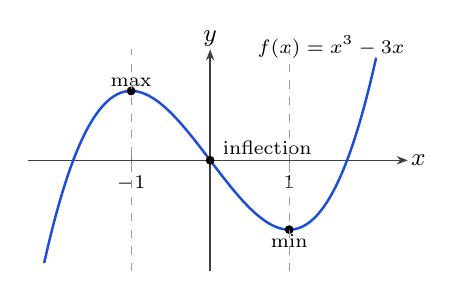
\begin{tikzpicture}
\begin{axis}[mygraph, width=6.4cm, height=4.4cm, xmin=-2.3, xmax=2.5, ymin=-3.2, ymax=3.2, xtick={-1,1}, ytick=\empty, cornertitle, title={$f(x)=x^3-3x$}]
  \addplot[plotA, domain=-2.1:2.1] {x^3-3*x};
  \node[pt] at (axis cs:-1,2) {}; \node[lab, above] at (axis cs:-1,2) {max};
  \node[pt] at (axis cs:1,-2) {}; \node[lab, below] at (axis cs:1,-2) {min};
  \node[pt] at (axis cs:0,0) {}; \node[lab, right] at (axis cs:0.1,0.35) {inflection};
  \draw[dashed, black!40] (axis cs:-1,-3.2) -- (axis cs:-1,3.2);
  \draw[dashed, black!40] (axis cs:1,-3.2) -- (axis cs:1,3.2);
\end{axis}
\end{tikzpicture}

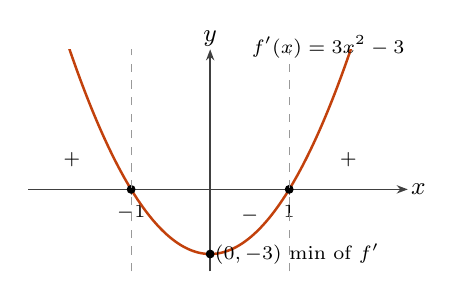
\begin{tikzpicture}
\begin{axis}[mygraph, width=6.4cm, height=4.4cm, xmin=-2.3, xmax=2.5, ymin=-3.8, ymax=6.5, xtick={-1,1}, ytick=\empty, cornertitle, title={$f'(x)=3x^2-3$}]
  \addplot[plotB, domain=-2.1:2.1] {3*x^2-3};
  \node[pt] at (axis cs:-1,0) {}; \node[pt] at (axis cs:1,0) {};
  \node[pt] at (axis cs:0,-3) {}; \node[lab, right] at (axis cs:0,-3) {$(0,-3)$ min of $f'$};
  \draw[dashed, black!40] (axis cs:-1,-3.8) -- (axis cs:-1,6.5);
  \draw[dashed, black!40] (axis cs:1,-3.8) -- (axis cs:1,6.5);
  \node[lab] at (axis cs:-1.75,1.4) {$+$};
  \node[lab] at (axis cs:1.75,1.4) {$+$};
  \node[lab] at (axis cs:0.5,-1.2) {$-$};
\end{axis}
\end{tikzpicture}
\end{cols}

% -----------------------------------------------------------------
\subsection{Stationary points, points of inflection, increasing and decreasing}
\label{sec:sp}

\begin{keyres}{Classifying stationary points ($f'(a)=0$)}
\begin{cols}
\textbf{Sign (gradient) test:} check $f'$ just either side of $a$.
\begin{itemize}
  \item $+\ \to\ 0\ \to\ -$: local \textbf{maximum}
  \item $-\ \to\ 0\ \to\ +$: local \textbf{minimum}
  \item $+\to0\to+$ or $-\to0\to-$: \textbf{stationary point of inflection}
\end{itemize}
\nextcol
\textbf{Second derivative test:}
\begin{itemize}
  \item $f''(a)<0$: local maximum (concave down)
  \item $f''(a)>0$: local minimum (concave up)
  \item $f''(a)=0$: \textbf{inconclusive}; use the sign test (e.g.\ $x^4$ has $f''(0)=0$ but a minimum at $0$)
\end{itemize}
\end{cols}
\textbf{Concavity:} $f''(x)>0$ concave up (gradient increasing); $f''(x)<0$ concave down. A \textbf{point of inflection} is where the concavity changes ($f''$ changes sign). There the gradient is a local max or min, so it is the \emph{steepest} point (``the rate of change is greatest/least''). It is a \emph{stationary} point of inflection if also $f'=0$.
\end{keyres}

\begin{defn}{Strictly increasing / decreasing}
$f$ is \textbf{strictly increasing} on an interval $I$ if $x_1<x_2\Rightarrow f(x_1)<f(x_2)$ for all $x_1,x_2\in I$ (strictly decreasing: $f(x_1)>f(x_2)$).
\begin{itemize}
  \item $f'(x)>0$ on an interval $\Rightarrow$ strictly increasing there. The converse fails: $x^3$ is strictly increasing on $\R$ although $f'(0)=0$.
  \item Using the definition, endpoints where $f'=0$ may be included: give the largest intervals, e.g.\ $f(x)=x^2$ is strictly increasing on $[0,\infty)$.
  \item Do \textbf{not} join intervals across an asymptote: $f(x)=\frac1x$ is strictly decreasing on $(-\infty,0)$ and on $(0,\infty)$, but not on $\R\setminus\{0\}$ (since $f(-1)<f(1)$).
\end{itemize}
\end{defn}

\begin{example}{full analysis of a cubic \byhand}
$f(x)=x^3-3x^2-9x+5$. \ $f'(x)=3x^2-6x-9=3(x-3)(x+1)$, \ $f''(x)=6x-6$.\par
\begin{tabular}{@{}l|ccccc@{}}
$x$ & $x<-1$ & $-1$ & $-1<x<3$ & $3$ & $x>3$\\ \hline
sign of $f'(x)$ & $+$ & $0$ & $-$ & $0$ & $+$\\
shape of $f$ & $\nearrow$ & max & $\searrow$ & min & $\nearrow$
\end{tabular}\par
Local maximum $(-1,10)$ [$f''(-1)=-12<0$]; local minimum $(3,-22)$ [$f''(3)=12>0$].\par
Point of inflection: $f''(x)=0\Rightarrow x=1$, and $f''$ changes sign, so $(1,-6)$, with gradient $f'(1)=-12$ (a non-stationary point of inflection).\par
Strictly increasing on $(-\infty,-1]$ and $[3,\infty)$; strictly decreasing on $[-1,3]$.
\end{example}

\begin{example}{a quartic with a stationary point of inflection}
$f(x)=x^4-4x^3$: \ $f'(x)=4x^2(x-3)$. At $x=0$: $f'$ is negative on both sides, so $(0,0)$ is a \textbf{stationary point of inflection}. At $x=3$: local minimum $(3,-27)$.\par
$f''(x)=12x(x-2)=0$ at $x=0$ and $x=2$. Both are points of inflection (sign changes): $(0,0)$ is stationary and $(2,-16)$ is non-stationary.
\end{example}

% -----------------------------------------------------------------
\subsection{Curve sketching with calculus}
\label{sec:sketch}

\begin{cols}[0.53]
\begin{method}{Checklist}
\begin{enumerate}
  \item Domain (maximal or given), endpoints.
  \item Axis intercepts.
  \item $f'(x)=0$ $\to$ stationary points, and their nature.
  \item $f''(x)=0$ with sign change $\to$ points of inflection (if asked).
  \item Asymptotes and behaviour as $x\to\pm\infty$ or near excluded points.
  \item Plot and label everything with coordinates. Use exact values unless told otherwise.
\end{enumerate}
\end{method}
\begin{example}{$f(x)=xe^{-x}$}
Intercept $(0,0)$. \ $f'(x)=e^{-x}-xe^{-x}=e^{-x}(1-x)$, so there is a maximum at $\left(1,\frac1e\right)$.\par
$f''(x)=e^{-x}(x-2)$, so there is a point of inflection at $\left(2,\frac{2}{e^2}\right)$.\par
As $x\to\infty$, $f(x)\to0^+$ (asymptote $y=0$); as $x\to-\infty$, $f(x)\to-\infty$. Range $\left(-\infty,\frac1e\right]$.
\end{example}
\nextcol[0.445]
\centering
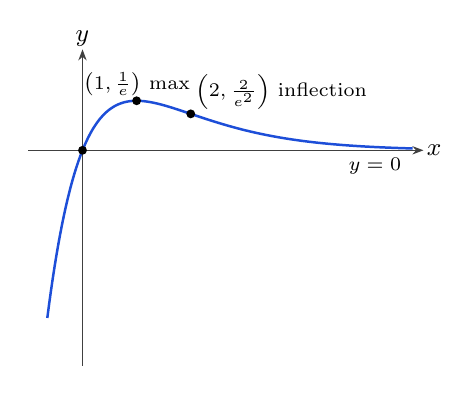
\begin{tikzpicture}
\begin{axis}[mygraph, width=6.6cm, height=5.6cm, xmin=-1.0, xmax=6.3, ymin=-1.6, ymax=0.75, xtick=\empty, ytick=\empty]
  \addplot[plotA, domain=-0.65:6.1] {x*exp(-x)};
  \node[pt] at (axis cs:1,0.3679) {}; \node[lab, above] at (axis cs:1,0.3679) {$\left(1,\frac1e\right)$ max};
  \node[pt] at (axis cs:2,0.2707) {}; \node[lab, above right] at (axis cs:2,0.2707) {$\left(2,\frac{2}{e^2}\right)$ inflection};
  \node[pt] at (axis cs:0,0) {};
  \node[lab] at (axis cs:5.4,-0.12) {$y=0$};
\end{axis}
\end{tikzpicture}
\end{cols}

% -----------------------------------------------------------------
\subsection{Absolute maximum and minimum; optimisation}
\label{sec:opt}

\begin{keyres}{Absolute (global) extrema on an interval}
On a closed interval $[a,b]$, the absolute maximum and minimum occur either at stationary points inside the interval \textbf{or at the endpoints}. Evaluate $f$ at all of them and compare. On an open interval, or with asymptotes, an absolute max/min may not exist. A \emph{local} max is not necessarily the absolute max.
\end{keyres}

\begin{example}{endpoint extrema \byhand}
$f(x)=x^3-3x$ on $[-2,3]$. Stationary points: $f'(x)=3x^2-3=0\Rightarrow x=\pm1$, giving $f(-1)=2$, $f(1)=-2$. Endpoints: $f(-2)=-2$, $f(3)=18$.\par
Absolute maximum $18$ (at the endpoint $x=3$); absolute minimum $-2$ (at $x=-2$ and $x=1$). Range $[-2,18]$.
\end{example}

\begin{method}{Optimisation problems}
\begin{enumerate}
  \item Draw a diagram and define the variables (with units).
  \item Write the quantity to optimise. Use the constraint to reduce it to \textbf{one variable}.
  \item State the \textbf{feasible domain} from the context (lengths $>0$, etc.).
  \item Differentiate and solve $=0$. Check the nature (sign test or $f''$) \textbf{and compare with the endpoints}.
  \item Answer the question asked, in context, with units.
\end{enumerate}
\end{method}

\begin{cols}
\begin{example}{open box \byhand}
Squares of side $x$ cm are cut from the corners of a $12\times12$ cm sheet, which is folded into an open box.\par
$V=x(12-2x)^2$, \ $0<x<6$.\par
$V'(x)=(12-2x)^2-4x(12-2x)=(12-2x)(12-6x)$.\par
$V'=0\Rightarrow x=2$ ($x=6$ is outside the domain). $V'$ changes from $+$ to $-$, so this is a maximum: $V(2)=2(8)^2=128$ cm$^3$.
\end{example}
\nextcol
\begin{example}{distance to a curve \examtwo}
Find the minimum distance from the origin to $y=e^x$.\par
$D(x)=\sqrt{x^2+e^{2x}}$. Minimise $D^2$ instead (same $x$): $\frac{d}{dx}(x^2+e^{2x})=2x+2e^{2x}=0$.\par
This can't be solved exactly by hand; CAS gives $x\approx-0.4263$, so $D_{\min}\approx0.7798$.\par
\textbf{Trick:} minimising $D^2$ avoids the square root.
\end{example}
\end{cols}

% -----------------------------------------------------------------
\subsection{Rates of change in context}
\label{sec:rates}

\begin{cols}
\begin{keyres}{Interpreting derivatives}
\begin{itemize}
  \item $\frac{dV}{dt}$ is the rate of change of $V$ with respect to $t$, in units of ($V$ units) per ($t$ unit), e.g.\ L/min.
  \item The sign says increasing or decreasing; the size says how fast.
  \item ``When is it increasing fastest?'' means maximise the rate: solve $\frac{d^2V}{dt^2}=0$ (a point of inflection of $V$).
  \item Chain rule for linked rates: $\frac{dy}{dt}=\frac{dy}{dx}\cdot\frac{dx}{dt}$.
  \item Motion: velocity $v=\frac{dx}{dt}$, acceleration $a=\frac{dv}{dt}$.
\end{itemize}
\end{keyres}
\nextcol
\begin{example}{rate of filling}
$V(t)=1000\left(1-e^{-0.1t}\right)$ litres after $t$ minutes.\par
$V'(t)=100e^{-0.1t}$ L/min, so the initial rate is $V'(0)=100$ L/min.\par
When is the rate $50$ L/min? $e^{-0.1t}=\frac12\Rightarrow t=10\loge2\approx6.93$ min.\par
$V'(t)>0$ always, and $V\to1000$: the tank approaches 1000 L but never reaches it.
\end{example}
\end{cols}

% -----------------------------------------------------------------
\subsection{Newton's method \newsd}
\label{sec:newton}

\begin{cols}[0.53]
\begin{keyres}{The algorithm (on the formula sheet)}
\[x_{n+1}=x_n-\frac{f(x_n)}{f'(x_n)}\]
Start with an estimate $x_0$ of a solution of $f(x)=0$. Each new estimate $x_{n+1}$ is the \textbf{$x$-intercept of the tangent} to $y=f(x)$ at $x=x_n$. Repeat until successive estimates agree to the required accuracy (e.g.\ $|x_{n+1}-x_n|<0.0001$).
\end{keyres}
\begin{warn}[When Newton's method fails or misbehaves]
\begin{itemize}
  \item $f'(x_n)=0$: the tangent is horizontal and never meets the axis (division by zero). E.g.\ $f(x)=x^3-3x+1$ with $x_0=1$.
  \item $f'(x_n)$ near $0$: the next estimate jumps far away, possibly converging to a different root.
  \item The estimates can oscillate (cycle) or diverge. A poor $x_0$ (near a turning point) is the usual cause. Choose $x_0$ close to the root, e.g.\ where $f$ changes sign.
\end{itemize}
\end{warn}
\nextcol[0.445]
\centering
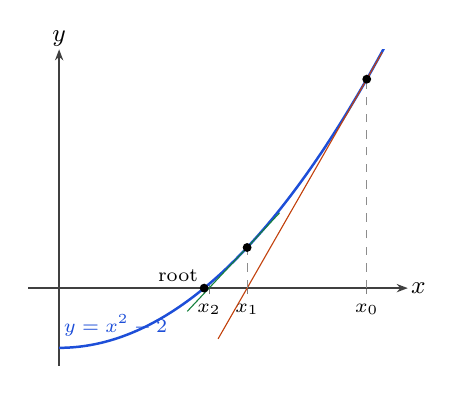
\begin{tikzpicture}
\begin{axis}[mygraph, width=6.4cm, height=5.6cm, xmin=-0.3, xmax=3.4, ymin=-2.6, ymax=8, xtick={1.4621,1.8333,3}, xticklabels={$x_2$,$x_1$,$x_0$}, ytick=\empty]
  \addplot[plotA, domain=0:3.25] {x^2-2};
  \addplot[plotB, thin, domain=1.55:3.15] {7+6*(x-3)};
  \addplot[plotC, thin, domain=1.25:2.15] {1.3611+3.6667*(x-1.8333)};
  \draw[dashed, black!45] (axis cs:3,0) -- (axis cs:3,7);
  \draw[dashed, black!45] (axis cs:1.8333,0) -- (axis cs:1.8333,1.3611);
  \node[pt] at (axis cs:3,7) {};
  \node[pt] at (axis cs:1.8333,1.3611) {};
  \node[pt] at (axis cs:1.4142,0) {};
  \node[lab, above left] at (axis cs:1.40,0.05) {root};
  \node[lab, plotA] at (axis cs:0.55,-1.25) {$y=x^2-2$};
\end{axis}
\end{tikzpicture}

{\scriptsize Each tangent's $x$-intercept is the next estimate: $3\to1.8333\to1.4621\to\dots\to\sqrt2$.}
\end{cols}

\begin{example}{Newton's method}
\textbf{(a) \byhand} Use $x_0=2$ to estimate $\sqrt5$ (a root of $f(x)=x^2-5$, $f'(x)=2x$):\par
$x_1=2-\frac{4-5}{4}=\frac94=2.25$; \quad $x_2=\frac94-\frac{\frac{81}{16}-5}{\frac92}=\frac94-\frac{1}{72}=\frac{161}{72}\approx2.23611$ (compare $\sqrt5\approx2.23607$).\par
\textbf{(b) \examtwo} Solve $x^3-2x-5=0$ with $x_0=2$, where $f'(x)=3x^2-2$:\par
\begin{tabular}{@{}cccc@{}}
$n$ & $x_n$ & $f(x_n)$ & $f'(x_n)$\\ \hline
0 & 2 & $-1$ & 10\\
1 & 2.1 & 0.061 & 11.23\\
2 & 2.094568 & 0.00018 & 11.16\\
3 & 2.094551 & & \\
\end{tabular}\quad The root is $2.0946$ (4 d.p.); successive estimates now agree.
\end{example}

% =================================================================
\section{Calculus II: anti-differentiation and integration (Area of Study 3)}
\label{sec:int}
% =================================================================

\begin{sdbox}
\begin{itemize}
  \item deducing the graph of an anti-derivative function from the graph of a given function
  \item anti-derivatives of polynomial functions and functions of the form $f(ax+b)$ where $f$ is $x^n$ for $n\in\Q$, $e^x$, $\sin(x)$, $\cos(x)$, and linear combinations of these
  \item informal consideration of the definite integral as a limiting value of a sum involving quantities such as area under a curve, and approximation of definite integrals using the \textbf{trapezium rule}
  \item anti-differentiation by recognition that $F'(x)=f(x)$ implies $\int f(x)\dx=F(x)+c$, and informal treatment of the fundamental theorem of calculus, $\int_a^bf(x)\dx=F(b)-F(a)$
  \item properties of anti-derivatives and definite integrals
  \item application of integration to finding a function from a known rate of change given a boundary condition, the area of a region under a curve and simple cases of areas between curves, the average value of a function, and other situations
\end{itemize}
\textbf{Key skills:} \byhand\ find anti-derivatives of polynomials, power functions, $f(ax+b)$ for $x^n$, $e^x$, sine and cosine, and linear combinations; evaluate trapezium-rule approximations; find and \emph{verify} anti-derivatives; evaluate definite integrals; find areas under and between curves.
\end{sdbox}

\subsection{Anti-derivatives (indefinite integrals)}
\label{sec:antideriv}

\begin{defn}{Definition}
$F$ is an \textbf{anti-derivative} of $f$ if $F'(x)=f(x)$. Then $\displaystyle\int f(x)\dx=F(x)+c$, where $c$ is an arbitrary constant. Anti-derivatives of $f$ form a \emph{family} of curves that differ by vertical translations. \textbf{Always check an anti-derivative by differentiating it.}
\end{defn}

\begin{cols}[0.5]
\begin{keyres}{Standard anti-derivatives}
\renewcommand{\arraystretch}{1.55}
\begin{tabular}{@{}l@{\quad}l@{}}
$f(x)$ & $\int f(x)\dx$ \\ \hline
$x^n$, $n\ne-1$ & $\dfrac{x^{n+1}}{n+1}+c$ \\
$(ax+b)^n$, $n\ne-1$ & $\dfrac{(ax+b)^{n+1}}{a(n+1)}+c$ \\
$\dfrac1x$ & $\loge(x)+c$, \ $x>0$ \\
$\dfrac{1}{ax+b}$ & $\dfrac1a\loge(ax+b)+c$, \ $ax+b>0$ \\
$e^{ax+b}$ & $\dfrac1ae^{ax+b}+c$ \\
$\sin(ax+b)$ & $-\dfrac1a\cos(ax+b)+c$ \\
$\cos(ax+b)$ & $\dfrac1a\sin(ax+b)+c$ \\
$\dfrac{1}{\cos^2(ax+b)}$\,$^{*}$ & $\dfrac1a\tan(ax+b)+c$ \\
\end{tabular}
\par\smallskip{\small $^{*}$by recognition (from the derivative of $\tan$).}
\end{keyres}
\nextcol[0.475]
\begin{keyres}{Properties of anti-derivatives}
\begin{itemize}
  \item $\int k\,f(x)\dx=k\int f(x)\dx$
  \item $\int\big(f(x)\pm g(x)\big)\dx=\int f(x)\dx\pm\int g(x)\dx$
  \item There is \textbf{no} product, quotient or chain rule for integrals in Methods: $\int f(x)g(x)\dx\ne\int f\dx\cdot\int g\dx$. Expand, simplify or use recognition instead.
  \item For $x<0$: $\int\frac1x\dx=\loge(-x)+c$; in general $\loge|x|+c$.
\end{itemize}
\end{keyres}
\begin{tip}[Rewrite first]
$\dfrac{x^2+1}{x^2}=1+x^{-2}$; \ $\sqrt x(x-1)=x^{3/2}-x^{1/2}$; \ $(e^x+1)^2=e^{2x}+2e^x+1$; \ $\dfrac{4}{\sqrt{2x+1}}=4(2x+1)^{-1/2}$.
\end{tip}
\end{cols}

\begin{example}{anti-differentiation \byhand}
\renewcommand{\arraystretch}{1.6}
\begin{tabularx}{\linewidth}{@{}>{$}l<{$}L@{}}
\int(3x^2-4x+5)\dx & $x^3-2x^2+5x+c$ \\
\int(2x+1)^4\dx & $\dfrac{(2x+1)^5}{2\times5}+c=\dfrac{(2x+1)^5}{10}+c$ \\
\int\dfrac{1}{\sqrt x}\dx=\int x^{-1/2}\dx & $\dfrac{x^{1/2}}{1/2}+c=2\sqrt x+c$ \\
\int\dfrac{4}{(1-2x)^3}\dx=4\int(1-2x)^{-3}\dx & $4\cdot\dfrac{(1-2x)^{-2}}{(-2)(-2)}+c=\dfrac{1}{(1-2x)^2}+c$ \\
\int e^{3x-1}\dx & $\frac13e^{3x-1}+c$ \\
\int\dfrac{2}{3x+1}\dx & $\frac23\loge(3x+1)+c$, \ $x>-\frac13$ \\
\int\sin(2x)\dx; \quad \int\cos\!\left(\frac x3\right)\dx & $-\frac12\cos(2x)+c$; \quad $3\sin\!\left(\frac x3\right)+c$ \\
\int\dfrac{x^2+1}{x^2}\dx=\int(1+x^{-2})\dx & $x-\dfrac1x+c$ \\
\end{tabularx}
\end{example}

\subsection{Anti-differentiation by recognition}
\label{sec:recog}

\begin{keyres}{The idea}
If you are told (or can show) that $\ddx\big(F(x)\big)=f(x)$, then $\int f(x)\dx=F(x)+c$. Typical question: ``Differentiate $g(x)$. \textbf{Hence} find an anti-derivative of $h(x)$.'' Rearrange the derivative so the part you need is on its own, then anti-differentiate both sides.
\end{keyres}

\begin{example}{recognition (very common in Exam 1) \byhand}
\textbf{(a)} $\ddx(x\loge x)=\loge x+1$. So $\int(\loge x+1)\dx=x\loge x$, which gives $\int\loge x\dx=x\loge x-\int1\dx=x\loge x-x+c$.\par
\textbf{(b)} $\ddx(x\cos x)=\cos x-x\sin x$. So $x\sin x=\cos x-\ddx(x\cos x)$, which gives $\int x\sin x\dx=\sin x-x\cos x+c$.\par
\textbf{(c)} $\ddx\left(e^{x^2}\right)=2xe^{x^2}$, so $\int xe^{x^2}\dx=\frac12e^{x^2}+c$.\par
\textbf{(d)} Using (a): $\int_1^e\loge x\dx=\big[x\loge x-x\big]_1^e=(e-e)-(0-1)=1$.\par
\textbf{Check} each by differentiating, e.g.\ $\ddx(\sin x-x\cos x)=\cos x-\cos x+x\sin x=x\sin x$. \tick
\end{example}

\subsection{Finding a function from its rate of change}
\label{sec:bc}

\begin{example}{boundary (initial) conditions \byhand}
\textbf{(a)} $f'(x)=6x^2-2x$ and $f(1)=4$: \ $f(x)=2x^3-x^2+c$; \ $2-1+c=4\Rightarrow c=3$, so $f(x)=2x^3-x^2+3$.\par
\textbf{(b)} $\dydx=\dfrac{1}{2x-1}$, $x>\frac12$, and $y=2$ when $x=1$: \ $y=\frac12\loge(2x-1)+c$; \ $\frac12\loge1+c=2\Rightarrow c=2$, so $y=\frac12\loge(2x-1)+2$.\par
\textbf{(c)} $f'(x)=\cos(2x)$ and $f\!\left(\frac{\pi}{4}\right)=1$: \ $f(x)=\frac12\sin(2x)+c$; \ $\frac12+c=1\Rightarrow c=\frac12$, so $f(x)=\frac12\sin(2x)+\frac12$.
\end{example}

\subsection{The graph of an anti-derivative from the graph of $f$}
\label{sec:antigraph}

\begin{cols}[0.5]
\begin{keyres}{Reading $F$ from $f=F'$}
\small
\begin{tabular}{@{}p{3.4cm}p{3.5cm}@{}}
\textbf{Graph of $f$} & \textbf{Graph of $F$ (anti-derivative)} \\ \hline
$x$-intercept with sign change & stationary point (turning point) of $F$ \\
$f>0$ & $F$ increasing \\
$f<0$ & $F$ decreasing \\
turning point of $f$ & point of inflection of $F$ \\
touches the $x$-axis & stationary point of inflection \\
degree $n$ polynomial & degree $n+1$ \\
\end{tabular}
\par\smallskip
(Figure: $c=-1,0,1$.) $F$ is only determined up to $+c$: sketch \emph{one} member of the family unless a point is given. The signed area under $f$ from $a$ to $b$ equals $F(b)-F(a)$, the \emph{change} in height of $F$.
\end{keyres}
\nextcol[0.475]
\centering
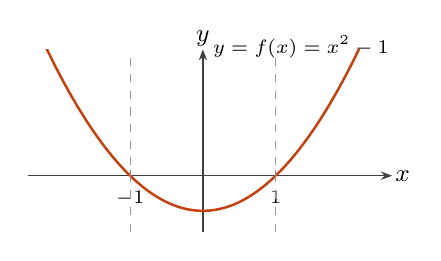
\begin{tikzpicture}
\begin{axis}[mygraph, width=6.2cm, height=3.9cm, xmin=-2.4, xmax=2.6, ymin=-1.6, ymax=3.6, xtick={-1,1}, ytick=\empty, cornertitle, title={$y=f(x)=x^2-1$}]
  \addplot[plotB, domain=-2.2:2.2] {x^2-1};
  \draw[dashed, black!40] (axis cs:-1,-1.6) -- (axis cs:-1,3.6);
  \draw[dashed, black!40] (axis cs:1,-1.6) -- (axis cs:1,3.6);
\end{axis}
\end{tikzpicture}

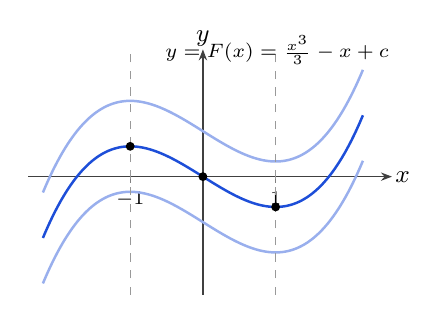
\begin{tikzpicture}
\begin{axis}[mygraph, width=6.2cm, height=4.7cm, xmin=-2.4, xmax=2.6, ymin=-2.6, ymax=2.8, xtick={-1,1}, ytick=\empty, cornertitle, title={$y=F(x)=\frac{x^3}{3}-x+c$}]
  \addplot[plotA!45, domain=-2.2:2.2] {x^3/3-x-1};
  \addplot[plotA, domain=-2.2:2.2] {x^3/3-x};
  \addplot[plotA!45, domain=-2.2:2.2] {x^3/3-x+1};
  \draw[dashed, black!40] (axis cs:-1,-2.6) -- (axis cs:-1,2.8);
  \draw[dashed, black!40] (axis cs:1,-2.6) -- (axis cs:1,2.8);
  \node[pt] at (axis cs:-1,0.6667) {}; \node[pt] at (axis cs:1,-0.6667) {};
  \node[pt] at (axis cs:0,0) {};
\end{axis}
\end{tikzpicture}
\end{cols}

% -----------------------------------------------------------------
\subsection{Definite integrals and the fundamental theorem of calculus}
\label{sec:definite}

\begin{keyres}{Fundamental theorem of calculus (informal)}
If $F'(x)=f(x)$ on $[a,b]$ (with $f$ continuous), then
\[\int_a^bf(x)\dx=\Big[F(x)\Big]_a^b=F(b)-F(a).\]
No $+c$ is needed (it cancels). The definite integral is a \textbf{number}: the \textbf{signed area} between $y=f(x)$ and the $x$-axis from $x=a$ to $x=b$. Area above the axis counts as positive, area below as negative. Also $\displaystyle\ddx\int_a^xf(t)\,dt=f(x)$, and $\displaystyle\int_a^bf'(x)\dx=f(b)-f(a)$ (net change).
\end{keyres}

\begin{cols}
\begin{keyres}{Properties of definite integrals}
\begin{itemize}
  \item $\int_a^af(x)\dx=0$; \ $\int_b^af(x)\dx=-\int_a^bf(x)\dx$
  \item $\int_a^bkf(x)\dx=k\int_a^bf(x)\dx$; \ $\int_a^bc\dx=c(b-a)$
  \item $\int_a^b(f\pm g)\dx=\int_a^bf\dx\pm\int_a^bg\dx$
  \item $\int_a^bf\dx+\int_b^cf\dx=\int_a^cf\dx$
  \item Translation: $\int_a^bf(x-h)\dx=\int_{a-h}^{b-h}f(x)\dx$
  \item Dilation: $\int_a^bf(kx)\dx=\frac1k\int_{ka}^{kb}f(x)\dx$
  \item Odd $f$: $\int_{-a}^af\dx=0$; \ even $f$: $\int_{-a}^af\dx=2\int_0^af\dx$
\end{itemize}
\end{keyres}
\nextcol
\begin{example}{using properties \mcq}
Given $\int_1^4f(x)\dx=5$:
\begin{itemize}
  \item $\int_1^4\big(2f(x)+3\big)\dx=2(5)+3(4-1)=19$
  \item $\int_4^1f(x)\dx=-5$
  \item $\int_1^4\big(f(x)-x\big)\dx=5-\left[\frac{x^2}{2}\right]_1^4=5-7.5=-2.5$
  \item $\int_0^3f(x+1)\dx=\int_1^4f(x)\dx=5$ (translation)
  \item $\int_{1/2}^{2}f(2x)\dx=\frac12\int_1^4f(x)\dx=\frac52$ (dilation)
\end{itemize}
\end{example}
\end{cols}

\begin{example}{evaluating definite integrals \byhand}
$\int_0^{\pi/2}\sin(2x)\dx=\left[-\tfrac12\cos(2x)\right]_0^{\pi/2}=-\tfrac12(\cos\pi-\cos0)=1$ \qquad
$\int_1^4\sqrt x\dx=\left[\tfrac23x^{3/2}\right]_1^4=\tfrac23(8-1)=\tfrac{14}{3}$\par
$\int_0^1e^{2x}\dx=\left[\tfrac12e^{2x}\right]_0^1=\tfrac{e^2-1}{2}$ \qquad
$\int_1^e\tfrac1x\dx=\big[\loge x\big]_1^e=1-0=1$
\end{example}

% -----------------------------------------------------------------
\subsection{The definite integral as a limit of sums; the trapezium rule}
\label{sec:trap}

\begin{cols}[0.55]
\begin{keyres}{Approximating area}
Split $[a,b]$ into $n$ strips of width $h=\dfrac{b-a}{n}$, with $x_i=a+ih$.
\begin{itemize}
  \item \textbf{Left/right rectangles:} $h\big[f(x_0)+\dots+f(x_{n-1})\big]$ or $h\big[f(x_1)+\dots+f(x_n)\big]$. For an increasing $f$, left rectangles under-estimate and right rectangles over-estimate.
  \item \textbf{Trapezium rule} (on the formula sheet):
  \[\int_a^bf(x)\dx\approx\frac{h}{2}\Big[f(x_0)+2f(x_1)+\dots+2f(x_{n-1})+f(x_n)\Big]\]
  (the formula sheet writes $\frac h2$ as $\frac{b-a}{2n}$). It equals the average of the left and right rectangle sums.
  \item \textbf{Concave up} ($f''>0$): the trapezium rule \textbf{over-estimates}. \textbf{Concave down}: it \textbf{under-estimates}.
  \item As $n\to\infty$ (strip width $\to0$), these sums approach the exact value: $\int_a^bf(x)\dx=\lim\sum f(x_i)\,\delta x$.
\end{itemize}
\end{keyres}
\nextcol[0.425]
\centering
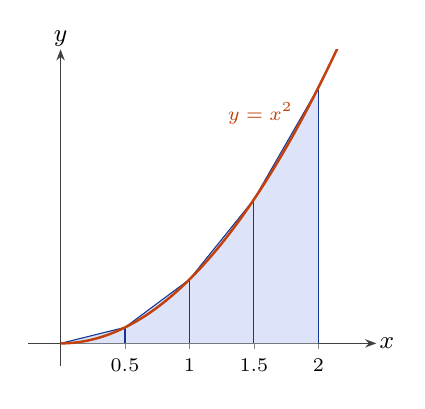
\begin{tikzpicture}
\begin{axis}[mygraph, width=6.0cm, height=5.6cm, xmin=-0.25, xmax=2.45, ymin=-0.35, ymax=4.6, xtick={0.5,1,1.5,2}, ytick=\empty]
  \fill[plotA!15] (axis cs:0,0) -- (axis cs:0,0) -- (axis cs:0.5,0.25) -- (axis cs:1,1) -- (axis cs:1.5,2.25) -- (axis cs:2,4) -- (axis cs:2,0) -- cycle;
  \draw[plotA!70!black, thin] (axis cs:0,0) -- (axis cs:0.5,0.25) -- (axis cs:1,1) -- (axis cs:1.5,2.25) -- (axis cs:2,4);
  \draw[plotA!70!black, thin] (axis cs:0.5,0) -- (axis cs:0.5,0.25);
  \draw[plotA!70!black, thin] (axis cs:1,0) -- (axis cs:1,1);
  \draw[plotA!70!black, thin] (axis cs:1.5,0) -- (axis cs:1.5,2.25);
  \draw[plotA!70!black, thin] (axis cs:2,0) -- (axis cs:2,4);
  \addplot[plotB, domain=0:2.2] {x^2};
  \node[lab, plotB] at (axis cs:1.55,3.6) {$y=x^2$};
\end{axis}
\end{tikzpicture}

{\scriptsize Four trapezia under $y=x^2$ on $[0,2]$. The curve is concave up, so the trapezia lie above it: an over-estimate.}
\end{cols}

\begin{example}{trapezium rule \byhand}
Estimate $\int_0^2x^2\dx$ using four strips ($h=0.5$).\par
\begin{tabular}{@{}l|ccccc@{}}
$x$ & $0$ & $0.5$ & $1$ & $1.5$ & $2$\\ \hline
$f(x)=x^2$ & $0$ & $0.25$ & $1$ & $2.25$ & $4$
\end{tabular}\par
Trapezium: $\frac{0.5}{2}\big[0+2(0.25+1+2.25)+4\big]=0.25\times11=2.75$. Exact value $\frac83\approx2.667$, so this is an over-estimate (concave up) \tick. Left rectangles give $0.5(0+0.25+1+2.25)=1.75$, right rectangles $0.5(0.25+1+2.25+4)=3.75$, and their average is $2.75$.\par
\textbf{Another:} $\int_1^3\frac1x\dx$ with $h=0.5$ gives $\frac{0.5}{2}\left[1+2\left(\frac23+\frac12+\frac25\right)+\frac13\right]=\frac{67}{60}\approx1.1167$, against the exact $\loge3\approx1.0986$.
\end{example}

% -----------------------------------------------------------------
\subsection{Areas under and between curves}
\label{sec:area}

\begin{method}{Finding an area}
\begin{enumerate}
  \item \textbf{Sketch.} Find the $x$-intercepts in the interval, or the intersection points of the curves.
  \item Area \emph{under} $y=f(x)$: if $f\ge0$, $A=\int_a^bf(x)\dx$; if $f\le0$, $A=-\int_a^bf(x)\dx$. If $f$ changes sign, \textbf{split at the $x$-intercepts} and add the absolute values.
  \item Area \emph{between} curves, with $f(x)\ge g(x)$ on $[a,b]$: $A=\displaystyle\int_a^b\big(f(x)-g(x)\big)\dx$ (top minus bottom; it does not matter which side of the $x$-axis the curves are on). If the curves cross inside the interval, split at the crossing.
\end{enumerate}
\end{method}

\begin{cols}
\begin{example}{signed area vs area \byhand}
$y=x^2-2x$ on $[0,3]$ (zeros at $0$ and $2$):\par
$\int_0^2(x^2-2x)\dx=\left[\frac{x^3}{3}-x^2\right]_0^2=-\frac43$\par
$\int_2^3(x^2-2x)\dx=0-\left(-\frac43\right)=\frac43$\par
Total \textbf{area} $=\frac43+\frac43=\frac83$, but $\int_0^3(x^2-2x)\dx=0$. The two regions cancel in the integral.
\end{example}
\nextcol
\centering
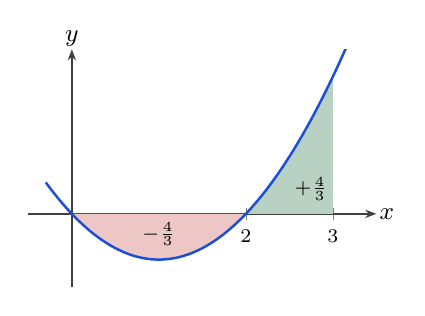
\begin{tikzpicture}
\begin{axis}[mygraph, width=6.0cm, height=4.6cm, xmin=-0.5, xmax=3.5, ymin=-1.6, ymax=3.6, xtick={2,3}, ytick=\empty]
  \addplot[name path=f, plotA, domain=-0.3:3.25] {x^2-2*x};
  \path[name path=ax] (axis cs:-0.5,0) -- (axis cs:3.5,0);
  \addplot[errcol!25] fill between[of=f and ax, soft clip={domain=0:2}];
  \addplot[excol!30] fill between[of=f and ax, soft clip={domain=2:3}];
  \node[lab] at (axis cs:1,-0.45) {$-\frac43$};
  \node[lab] at (axis cs:2.75,0.55) {$+\frac43$};
\end{axis}
\end{tikzpicture}
\end{cols}

\begin{cols}
\begin{example}{area between curves \byhand}
Area enclosed by $y=x^2$ and $y=x+2$.\par
Intersections: $x^2=x+2\Rightarrow(x-2)(x+1)=0$, so $x=-1,2$.\par
On $[-1,2]$ the line is on top:\par
$A=\int_{-1}^2(x+2-x^2)\dx=\left[\frac{x^2}{2}+2x-\frac{x^3}{3}\right]_{-1}^2$\par
$=\frac{10}{3}-\left(-\frac76\right)=\frac92$ square units.
\end{example}
\nextcol
\centering
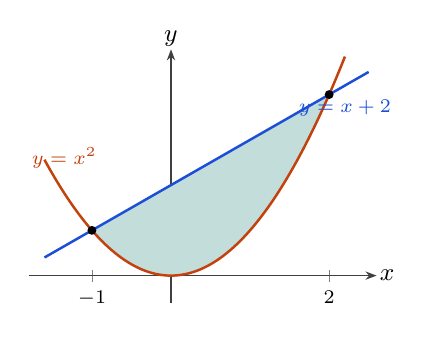
\begin{tikzpicture}
\begin{axis}[mygraph, width=6.0cm, height=4.8cm, xmin=-1.8, xmax=2.6, ymin=-0.6, ymax=5.0, xtick={-1,2}, ytick=\empty]
  \addplot[name path=g, plotB, domain=-1.6:2.2] {x^2};
  \addplot[name path=h, plotA, domain=-1.6:2.5] {x+2};
  \addplot[keycol!25] fill between[of=h and g, soft clip={domain=-1:2}];
  \node[pt] at (axis cs:-1,1) {}; \node[pt] at (axis cs:2,4) {};
  \node[lab, plotA] at (axis cs:2.2,3.7) {$y=x+2$};
  \node[lab, plotB] at (axis cs:-1.35,2.6) {$y=x^2$};
\end{axis}
\end{tikzpicture}
\end{cols}

\begin{example}{circular functions and areas \byhand}
Area between $y=\sin x$ and $y=\cos x$ from $x=\frac{\pi}{4}$ to $x=\frac{5\pi}{4}$ (they meet at both ends, and $\sin x\ge\cos x$ in between):\par
$A=\int_{\pi/4}^{5\pi/4}(\sin x-\cos x)\dx=\big[-\cos x-\sin x\big]_{\pi/4}^{5\pi/4}=\left(\tfrac{\sqrt2}{2}+\tfrac{\sqrt2}{2}\right)-\left(-\tfrac{\sqrt2}{2}-\tfrac{\sqrt2}{2}\right)=2\sqrt2$.
\end{example}

\begin{tip}[Areas involving inverse functions and the $y$-axis]
\begin{itemize}
  \item The area between $f$ and $f^{-1}$ (meeting on $y=x$) is \textbf{twice} the area between $f$ and $y=x$.
  \item For increasing $f$: $\displaystyle\int_{f(a)}^{f(b)}f^{-1}(x)\dx=bf(b)-af(a)-\int_a^bf(x)\dx$ (rectangle subtraction). For example, $\int_1^e\loge x\dx=1\cdot e-0-\int_0^1e^x\dx=e-(e-1)=1$.
  \item An area between a curve and the $y$-axis can be found as a rectangle minus an area with respect to $x$. Draw the diagram.
\end{itemize}
\end{tip}

% -----------------------------------------------------------------
\subsection{Average value of a function}
\label{sec:avg}

\begin{cols}[0.6]
\begin{keyres}{Average value}
The average value of $f$ over $[a,b]$ is
\[\bar f=\frac{1}{b-a}\int_a^bf(x)\dx.\]
It is the height of the rectangle on $[a,b]$ that has the same (signed) area as the region under the curve.\par
\textbf{Do not confuse} it with the \emph{average rate of change} $\frac{f(b)-f(a)}{b-a}$. For $f(x)=x^2$ on $[0,2]$: average value $=\frac12\cdot\frac83=\frac43$, but average rate of change $=\frac{4-0}{2}=2$.
\end{keyres}
\begin{example}{average value \byhand}
Average value of $\sin x$ over $[0,\pi]$: $\frac{1}{\pi}\int_0^\pi\sin x\dx=\frac1\pi\big[-\cos x\big]_0^\pi=\frac{2}{\pi}$.
\end{example}
\nextcol[0.37]
\centering
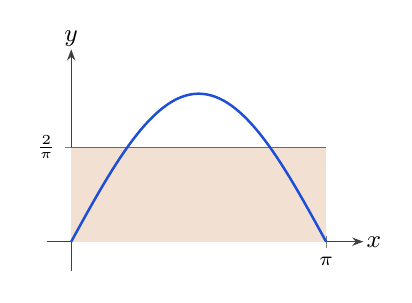
\begin{tikzpicture}
\begin{axis}[mygraph, width=5.6cm, height=4.4cm, xmin=-0.3, xmax=3.6, ymin=-0.2, ymax=1.3, xtick={3.14159}, xticklabels={$\pi$}, ytick={0.6366}, yticklabels={$\frac{2}{\pi}$}]
  \fill[tipcol!18] (axis cs:0,0) rectangle (axis cs:3.14159,0.6366);
  \draw[tipcol, thin] (axis cs:0,0.6366) -- (axis cs:3.14159,0.6366);
  \addplot[plotA, domain=0:3.14159] {sin(deg(x))};
\end{axis}
\end{tikzpicture}

{\scriptsize The rectangle of height $\frac2\pi$ has the same area ($2$) as the region under $\sin x$.}
\end{cols}

% -----------------------------------------------------------------
\subsection{Other applications: net change, motion, probability}
\label{sec:apps}

\begin{cols}
\begin{keyres}{Integrating a rate}
\begin{itemize}
  \item If $R(t)=\frac{dQ}{dt}$ is a rate, the \textbf{total change} in $Q$ from $t=a$ to $t=b$ is $\int_a^bR(t)\,dt=Q(b)-Q(a)$.
  \item Motion: displacement $=\int_{t_1}^{t_2}v\,dt$; distance travelled $=\int_{t_1}^{t_2}|v|\,dt$ (split where $v=0$).
  \item Probability: for a continuous random variable, $\Pr(a<X<b)=\int_a^bf(x)\dx$ (see \S\ref{sec:crv}).
\end{itemize}
\end{keyres}
\nextcol
\begin{example}{total change}
Water flows into a tank at $R(t)=20-4t$ L/min for $0\le t\le5$. The volume added is
$\int_0^5(20-4t)\,dt=\big[20t-2t^2\big]_0^5=100-50=50$ L.
\end{example}
\begin{cas}
Use the integral template with exact bounds. To \emph{find a bound}, solve, e.g.\ \texttt{solve}$\left(\int_0^kf(x)\,dx=2,\,k\right)$ with a domain restriction. To check a total area, integrate $|f(x)|$. Graph first to see the sign changes.
\end{cas}
\end{cols}

% =================================================================
\section{Random variables and probability distributions (Area of Study 4)}
\label{sec:rv}
% =================================================================

\begin{sdbox}
\begin{itemize}
  \item random variables, including the concept of a random variable as a real function defined on a sample space, and examples of discrete and continuous random variables
  \item \textbf{discrete random variables:} specification of probability distributions using graphs, tables and probability mass functions; calculation and interpretation of mean $\mu$, variance $\sigma^2$ and standard deviation, and their use; \textbf{Bernoulli trials and the binomial distribution} $\Bi(n,p)$; effect of variation in the value(s) of defining parameters on the graph of a probability mass function; calculation of probabilities for specific values and intervals, \textbf{including conditional probability}
  \item \textbf{continuous random variables:} construction of probability density functions from non-negative functions of a real variable; specification of probability distributions using pdfs; calculation and interpretation of $\mu$, $\sigma^2$ and $\sigma$, and their use; the \textbf{standard normal} $\Nd(0,1)$ and transformed normal distributions $\Nd(\mu,\sigma^2)$; effect of variation in the defining parameters on the graph of a pdf; calculation of probabilities for intervals, \textbf{including conditional probability} (the cumulative distribution function may be used but is not required)
\end{itemize}
\textbf{Key knowledge/skills:} the conditions under which a Bernoulli trial or a probability distribution may be selected to model a situation; analyse a pmf or pdf and its graph in terms of its parameters, mean and variance; calculate and interpret probabilities \byhand\ where the arithmetic is simple; apply distributions to modelling and problem solving.
\end{sdbox}

\subsection{Random variables}
\label{sec:rvdef}

\begin{cols}
\begin{defn}{Random variables}
A \textbf{random variable} $X$ is a function that assigns a real number to each outcome in the sample space of a random experiment. Upper case $X$ is the variable; lower case $x$ is a particular value.
\begin{itemize}
  \item \textbf{Discrete:} countable values, e.g.\ number of heads, number of faulty items, goals scored.
  \item \textbf{Continuous:} any value in an interval, e.g.\ time, height, mass, temperature.
\end{itemize}
\end{defn}
\nextcol
\begin{example}{a random variable from a sample space}
Toss two fair coins; $X$ = number of heads. Sample space $\{HH,HT,TH,TT\}$, so $X$ takes the values $2,1,1,0$.\par
\begin{tabular}{@{}l|ccc@{}}
$x$ & $0$ & $1$ & $2$\\ \hline
$\Pr(X=x)$ & $\frac14$ & $\frac12$ & $\frac14$
\end{tabular}\par
$\E(X)=0+\frac12+\frac12=1$.
\end{example}
\end{cols}

% -----------------------------------------------------------------
\subsection{Discrete probability distributions}
\label{sec:discrete}

\begin{keyres}{Discrete random variables}
\begin{cols}
\begin{itemize}
  \item \textbf{pmf:} $p(x)=\Pr(X=x)$, given by a table, a graph or a rule.
  \item \textbf{Conditions:} $0\le p(x)\le1$ for every $x$, and $\sum p(x)=1$.
  \item \textbf{Mean} (expected value, the long-run average):\\ $\mu=\E(X)=\sum x\,p(x)$; in general $\E(g(X))=\sum g(x)\,p(x)$.
  \item \textbf{Variance:} $\sigma^2=\Var(X)=\E\big[(X-\mu)^2\big]=\E(X^2)-\mu^2$.
  \item \textbf{Standard deviation:} $\sigma=\sd(X)=\sqrt{\Var(X)}$, in the same units as $X$.
\end{itemize}
\nextcol
\begin{itemize}
  \item \textbf{Linear change:} $\E(aX+b)=a\E(X)+b$; \ $\Var(aX+b)=a^2\Var(X)$; \ $\sd(aX+b)=|a|\sd(X)$. Adding a constant shifts the mean but not the spread.
  \item \textbf{Mode:} the most probable value. \textbf{Median:} the value where the cumulative probability first reaches $0.5$.
  \item For many distributions, about 95\% of values lie within $\mu\pm2\sigma$ (a rule of thumb).
  \item \textbf{Conditional:} $\Pr(X\in A\mid X\in B)=\dfrac{\Pr(X\in A\cap B)}{\Pr(X\in B)}$.
\end{itemize}
\end{cols}
\end{keyres}

\begin{example}{a discrete distribution with an unknown \byhand}
\begin{tabular}{@{}l|cccc@{}}
$x$ & $0$ & $1$ & $2$ & $3$\\ \hline
$\Pr(X=x)$ & $0.1$ & $k$ & $2k$ & $0.3$
\end{tabular}\quad
\textbf{(a)} $0.1+k+2k+0.3=1\Rightarrow k=0.2$.\par
\textbf{(b)} $\E(X)=0(0.1)+1(0.2)+2(0.4)+3(0.3)=1.9$. \ $\E(X^2)=0+0.2+1.6+2.7=4.5$.\par
\phantom{\textbf{(b)}} $\Var(X)=4.5-1.9^2=0.89$, so $\sd(X)=\sqrt{0.89}\approx0.943$.\par
\textbf{(c)} $\Pr(X\ge2\mid X\ge1)=\dfrac{\Pr(X\ge2)}{\Pr(X\ge1)}=\dfrac{0.4+0.3}{0.9}=\dfrac79$.\par
\textbf{(d)} $\E(3X-2)=3(1.9)-2=3.7$; \ $\Var(3X-2)=9(0.89)=8.01$.\par
\textbf{(e)} Mode $=2$. Cumulative: $0.1,\,0.3,\,0.7,\dots$, so the median is $2$.\par
\textbf{(f)} Two independent observations: $\Pr(\text{sum}=2)=\Pr(0,2)+\Pr(2,0)+\Pr(1,1)=2(0.1)(0.4)+(0.2)^2=0.12$.
\end{example}

\begin{tip}[\mcq{} Discrete inequalities]
For integer-valued $X$: $\Pr(X<3)=\Pr(X\le2)$, \ $\Pr(X>3)=\Pr(X\ge4)=1-\Pr(X\le3)$. ``At least 3'' is $X\ge3$; ``more than 3'' is $X\ge4$; ``at most 3'' / ``no more than 3'' is $X\le3$; ``fewer than 3'' is $X\le2$. For a rule-based pmf, check the conditions (e.g.\ $\Pr(X=x)=\frac{x}{10}$, $x\in\{1,2,3,4\}$, sums to $1$; its mean is $\frac{1+4+9+16}{10}=3$).
\end{tip}

% -----------------------------------------------------------------
\subsection{Bernoulli trials and the binomial distribution}
\label{sec:binomial}

\begin{keyres}{The binomial distribution $X\sim\Bi(n,p)$}
\begin{cols}
\textbf{Bernoulli trial:} one trial with two outcomes, success (probability $p$) or failure ($1-p$). A Bernoulli variable takes the values $1$ or $0$, with mean $p$ and variance $p(1-p)$.\par
\textbf{Binomial conditions} (state these when asked to justify the model):
\begin{enumerate}
  \item a fixed number $n$ of trials;
  \item each trial has two outcomes (success/failure);
  \item the trials are independent;
  \item $p$ is the same for every trial.
\end{enumerate}
$X$ = the number of successes in $n$ trials.
\nextcol
\[\Pr(X=x)=\binom{n}{x}p^x(1-p)^{n-x},\quad x=0,1,\dots,n\]
\[\E(X)=np,\qquad\Var(X)=np(1-p)\]
\[\sd(X)=\sqrt{np(1-p)}\]
\textbf{Not binomial:} sampling \emph{without replacement} from a small population ($p$ changes and the trials are not independent); trials that affect each other; ``repeat until the first success'' (the number of trials isn't fixed).\par
\textbf{Mode:} the most likely value, near $np$ (for $\Bi(20,0.3)$ it is $6$).
\end{cols}
\end{keyres}

\begin{center}
\pgfplotsset{binom/.style={smallgraph, width=5.3cm, height=3.6cm, ybar, bar width=4.5pt, xmin=-0.8, xmax=10.8, ymin=0, ymax=0.33,
  xtick={0,2,4,6,8,10}, ytick={0.1,0.2,0.3}, axis lines=left, xlabel={$x$}, ylabel={},
  every axis plot/.append style={line width=0.4pt}, title style={font=\scriptsize}}}
\begin{tikzpicture}
\begin{axis}[binom, title={$\Bi(10,0.2)$: positively skewed}]
\addplot[fill=plotA!60, draw=plotA] coordinates {(0,0.1074) (1,0.2684) (2,0.3020) (3,0.2013) (4,0.0881) (5,0.0264) (6,0.0055) (7,0.0008) (8,0.0001) (9,0) (10,0)};
\end{axis}
\end{tikzpicture}\hfill
\begin{tikzpicture}
\begin{axis}[binom, title={$\Bi(10,0.5)$: symmetric}]
\addplot[fill=plotC!60, draw=plotC] coordinates {(0,0.0010) (1,0.0098) (2,0.0439) (3,0.1172) (4,0.2051) (5,0.2461) (6,0.2051) (7,0.1172) (8,0.0439) (9,0.0098) (10,0.0010)};
\end{axis}
\end{tikzpicture}\hfill
\begin{tikzpicture}
\begin{axis}[binom, title={$\Bi(10,0.8)$: negatively skewed}]
\addplot[fill=plotB!60, draw=plotB] coordinates {(0,0) (1,0) (2,0.0001) (3,0.0008) (4,0.0055) (5,0.0264) (6,0.0881) (7,0.2013) (8,0.3020) (9,0.2684) (10,0.1074)};
\end{axis}
\end{tikzpicture}

{\scriptsize\textbf{Effect of the parameters:} $p<0.5$ positively skewed, $p=0.5$ symmetric, $p>0.5$ negatively skewed. Increasing $n$ moves the centre ($np$) right, spreads the distribution and makes it more symmetric (bell-shaped).}
\end{center}

\begin{cols}
\begin{example}{binomial \byhand}
$X\sim\Bi\!\left(4,\frac13\right)$.\par
$\Pr(X=2)=\binom42\left(\frac13\right)^2\left(\frac23\right)^2=6\cdot\frac19\cdot\frac49=\frac{8}{27}$.\par
$\Pr(X\ge1)=1-\Pr(X=0)=1-\left(\frac23\right)^4=\frac{65}{81}$.\par
$\Pr(X=2\mid X\ge1)=\dfrac{8/27}{65/81}=\dfrac{24}{65}$.\par
$\E(X)=\frac43$, \ $\Var(X)=4\cdot\frac13\cdot\frac23=\frac89$.
\end{example}
\nextcol
\begin{example}{binomial with CAS \examtwo}
$X\sim\Bi(20,0.3)$.\par
$\Pr(X\ge5)=1-\Pr(X\le4)=1-0.2375=0.7625$ (CAS \texttt{binomCdf} from 5 to 20).\par
\textbf{Find $p$:} if $n=4$ and $\Pr(X=0)=0.0256$, then $(1-p)^4=0.0256$, so $1-p=0.4$ and $p=0.6$.\par
\textbf{From the mean and variance:} $np=6$ and $np(1-p)=4.2$ give $1-p=0.7$, so $p=0.3$ and $n=20$.
\end{example}
\end{cols}

\begin{example}{``at least one'': finding $n$}
Each item is faulty with probability $0.1$. How many items must be tested so that the probability of finding \emph{at least one} faulty item is more than $0.95$?\par
$\Pr(X\ge1)=1-0.9^n>0.95\Rightarrow0.9^n<0.05\Rightarrow n\loge(0.9)<\loge(0.05)\Rightarrow n>\dfrac{\loge0.05}{\loge0.9}\approx28.4$.\par
\textbf{The inequality flips} because $\loge0.9<0$. So $n=29$. Check: $0.9^{28}\approx0.052$ (too big) and $0.9^{29}\approx0.047$ \tick.
\end{example}

% -----------------------------------------------------------------
\subsection{Continuous random variables and probability density functions}
\label{sec:crv}

\begin{keyres}{Probability density functions}
\begin{cols}
\begin{itemize}
  \item $f$ is a \textbf{pdf} if (1) $f(x)\ge0$ for all $x$, and (2) $\displaystyle\int_{-\infty}^{\infty}f(x)\dx=1$ (total area $1$).
  \item $\Pr(a<X<b)=\displaystyle\int_a^bf(x)\dx$, the area under the pdf.
  \item $\Pr(X=a)=0$, so $\Pr(a<X<b)=\Pr(a\le X\le b)$: strict and non-strict inequalities give the same answer.
  \item \textbf{Constructing a pdf:} for $g(x)\ge0$ on $[a,b]$, the function $f(x)=kg(x)$ there (and $0$ elsewhere) is a pdf when $k=\dfrac{1}{\int_a^bg(x)\dx}$.
\end{itemize}
\nextcol
\begin{itemize}
  \item \textbf{Mean:} $\mu=\E(X)=\displaystyle\int_{-\infty}^{\infty}x\,f(x)\dx$.
  \item \textbf{Variance:} $\Var(X)=\displaystyle\int_{-\infty}^{\infty}(x-\mu)^2f(x)\dx=\E(X^2)-\mu^2$, with $\E(X^2)=\int x^2f(x)\dx$.
  \item \textbf{Median} $m$: $\displaystyle\int_{-\infty}^{m}f(x)\dx=0.5$. A percentile $q$: $\int_{-\infty}^qf(x)\dx=$ the given proportion.
  \item \textbf{Mode:} the $x$ where $f(x)$ is greatest (it can be at an endpoint).
  \item \textbf{Symmetric pdf:} mean = median = the centre of symmetry.
  \item CDF (optional): $F(x)=\Pr(X\le x)=\int_{-\infty}^xf(t)\,dt$, with $F'(x)=f(x)$.
\end{itemize}
\end{cols}
\end{keyres}

\begin{cols}[0.6]
\begin{example}{a polynomial pdf \byhand}
$f(x)=\begin{cases}kx(2-x), & 0\le x\le2\\0, & \text{elsewhere}\end{cases}$\par
\textbf{$k$:} $k\int_0^2(2x-x^2)\dx=k\left[x^2-\frac{x^3}{3}\right]_0^2=\frac{4k}{3}=1\Rightarrow k=\frac34$.\par
\textbf{Mean:} $1$ (by symmetry about $x=1$). \ $\E(X^2)=\frac34\int_0^2(2x^3-x^4)\dx=\frac34\left(8-\frac{32}{5}\right)=\frac65$.\par
$\Var(X)=\frac65-1^2=\frac15$, so $\sd(X)=\frac{1}{\sqrt5}$. Median and mode are $1$.\par
$\Pr(X<0.5)=\frac34\left[x^2-\frac{x^3}{3}\right]_0^{1/2}=\frac34\cdot\frac{5}{24}=\frac{5}{32}$.\par
$\Pr(X<1\mid X>0.5)=\dfrac{\Pr(0.5<X<1)}{\Pr(X>0.5)}=\dfrac{\frac12-\frac{5}{32}}{1-\frac{5}{32}}=\dfrac{11}{27}$.
\end{example}
\nextcol[0.37]
\centering
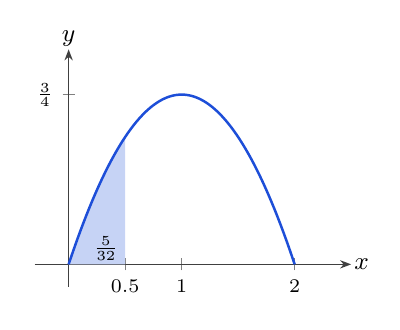
\begin{tikzpicture}
\begin{axis}[mygraph, width=5.6cm, height=4.6cm, xmin=-0.3, xmax=2.5, ymin=-0.1, ymax=0.95, xtick={0.5,1,2}, ytick={0.75}, yticklabels={$\frac34$}]
  \addplot[name path=p, plotA, domain=0:2] {0.75*x*(2-x)};
  \path[name path=ax] (axis cs:0,0) -- (axis cs:2,0);
  \addplot[plotA!25] fill between[of=p and ax, soft clip={domain=0:0.5}];
  \node[lab] at (axis cs:0.33,0.07) {$\frac{5}{32}$};
\end{axis}
\end{tikzpicture}

{\scriptsize The shaded area is $\Pr(X<0.5)=\frac{5}{32}$.}
\end{cols}

\begin{cols}
\begin{example}{median vs mean \byhand}
$f(x)=\frac x2$ on $[0,2]$ (and $0$ elsewhere). It is a pdf since $\int_0^2\frac x2\dx=1$.\par
Median: $\int_0^m\frac x2\dx=\frac{m^2}{4}=\frac12\Rightarrow m=\sqrt2$.\par
Mean: $\int_0^2\frac{x^2}{2}\dx=\frac43$. \ $\E(X^2)=\int_0^2\frac{x^3}{2}\dx=2$, so $\Var(X)=2-\frac{16}{9}=\frac29$.\par
The mean $\frac43\approx1.33$ is less than the median $\sqrt2\approx1.41$: the distribution is negatively skewed.
\end{example}
\nextcol
\begin{example}{an exponential pdf and a parameter}
$f(x)=ke^{-2x}$ for $x\ge0$: $\int_0^\infty ke^{-2x}\dx=\frac k2=1\Rightarrow k=2$.\par
Median: $\int_0^m2e^{-2x}\dx=1-e^{-2m}=\frac12\Rightarrow m=\frac{\loge2}{2}$.\par
CAS: $\E(X)=\frac12$, $\Var(X)=\frac14$.\par
\textbf{Parameter effect:} for $f(x)=\lambda e^{-\lambda x}$, a larger $\lambda$ gives a higher starting value ($f(0)=\lambda$), a faster decay and a smaller mean $\frac1\lambda$. The area stays $1$.
\end{example}
\end{cols}

\begin{tip}[Transformations and pdfs]
If $Y=aX+b$, then $\E(Y)=a\E(X)+b$ and $\Var(Y)=a^2\Var(X)$ (same as discrete). Translating a pdf by $h$ adds $h$ to the mean and median and leaves the variance unchanged. Dilating a pdf by factor $a$ from the $y$-axis requires a dilation by factor $\frac1a$ from the $x$-axis to keep the total area $1$: the new pdf is $\frac1af\!\left(\frac xa\right)$, with mean $\times a$ and variance $\times a^2$. For a hybrid pdf, integrate each piece over its own interval and add.
\end{tip}

% -----------------------------------------------------------------
\subsection{The normal distribution}
\label{sec:normal}

\begin{cols}[0.53]
\begin{keyres}{$X\sim\Nd(\mu,\sigma^2)$}
\begin{itemize}
  \item Bell-shaped and symmetric about $x=\mu$; mean = median = mode $=\mu$; points of inflection at $\mu\pm\sigma$; total area $1$.
  \item pdf: $f(x)=\dfrac{1}{\sigma\sqrt{2\pi}}\,e^{-\frac12\left(\frac{x-\mu}{\sigma}\right)^2}$ (rarely needed by hand).
  \item \textbf{The second parameter is the variance:} $\Nd(10,4)$ has $\sigma=2$.
  \item \textbf{Effect of parameters:} changing $\mu$ translates the curve; a larger $\sigma$ makes it wider and lower (peak height $\frac{1}{\sigma\sqrt{2\pi}}$).
  \item \textbf{Standard normal:} $Z\sim\Nd(0,1)$. Standardise with $Z=\dfrac{X-\mu}{\sigma}$. The $z$-score is the number of standard deviations from the mean.
  \item \textbf{68--95--99.7\% rule:} about 68\%, 95\% and 99.7\% of values lie within $1$, $2$ and $3$ standard deviations of $\mu$.
\end{itemize}
\end{keyres}
\nextcol[0.445]
\centering
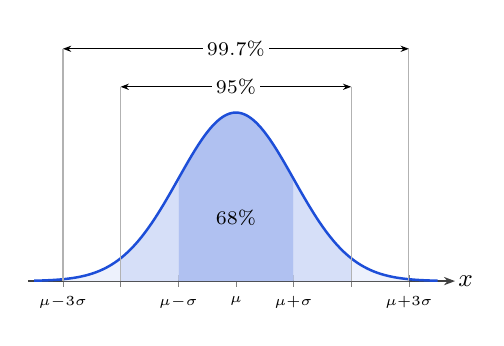
\begin{tikzpicture}[declare function={npdf(\x,\m,\s)=1/(\s*sqrt(2*pi))*exp(-((\x-\m)^2)/(2*\s^2));}]
\begin{axis}[mygraph, width=7.0cm, height=4.8cm, xmin=-3.6, xmax=3.8, ymin=0, ymax=0.6,
  xtick={-3,-2,-1,0,1,2,3}, xticklabels={$\mu{-}3\sigma$,,$\mu{-}\sigma$,$\mu$,$\mu{+}\sigma$,,$\mu{+}3\sigma$}, ytick=\empty, axis y line=none,
  every tick label/.append style={font=\tiny}]
  \addplot[name path=n, plotA, domain=-3.5:3.5] {npdf(x,0,1)};
  \path[name path=ax] (axis cs:-3.5,0) -- (axis cs:3.5,0);
  \addplot[plotA!35] fill between[of=n and ax, soft clip={domain=-1:1}];
  \addplot[plotA!18] fill between[of=n and ax, soft clip={domain=-2:-1}];
  \addplot[plotA!18] fill between[of=n and ax, soft clip={domain=1:2}];
  \addplot[plotA!8] fill between[of=n and ax, soft clip={domain=-3:-2}];
  \addplot[plotA!8] fill between[of=n and ax, soft clip={domain=2:3}];
  \node[lab] at (axis cs:0,0.15) {$68\%$};
  \draw[{Stealth[length=3pt]}-{Stealth[length=3pt]}, thin] (axis cs:-2,0.46) -- node[lab, fill=white] {$95\%$} (axis cs:2,0.46);
  \draw[{Stealth[length=3pt]}-{Stealth[length=3pt]}, thin] (axis cs:-3,0.55) -- node[lab, fill=white] {$99.7\%$} (axis cs:3,0.55);
  \draw[black!30, thin] (axis cs:-2,0) -- (axis cs:-2,0.46) (axis cs:2,0) -- (axis cs:2,0.46) (axis cs:-3,0) -- (axis cs:-3,0.55) (axis cs:3,0) -- (axis cs:3,0.55);
\end{axis}
\end{tikzpicture}

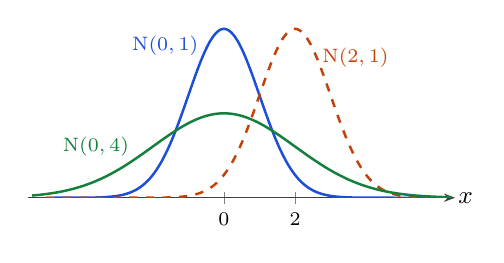
\begin{tikzpicture}[declare function={npdf(\x,\m,\s)=1/(\s*sqrt(2*pi))*exp(-((\x-\m)^2)/(2*\s^2));}]
\begin{axis}[mygraph, width=7.0cm, height=4.0cm, xmin=-5.5, xmax=6.5, ymin=0, ymax=0.45, xtick={0,2}, ytick=\empty, axis y line=none, every tick label/.append style={font=\scriptsize}]
  \addplot[plotA, domain=-5:6] {npdf(x,0,1)};
  \addplot[plotB, dashed, domain=-5:6] {npdf(x,2,1)};
  \addplot[plotC, domain=-5.4:6.4] {npdf(x,0,2)};
  \node[lab, plotA] at (axis cs:-1.65,0.36) {$\Nd(0,1)$};
  \node[lab, plotB] at (axis cs:3.7,0.33) {$\Nd(2,1)$};
  \node[lab, plotC] at (axis cs:-3.6,0.12) {$\Nd(0,4)$};
\end{axis}
\end{tikzpicture}
\end{cols}

\begin{keyres}{Symmetry results for $Z\sim\Nd(0,1)$ (essential for Exam 1)}
$\Pr(Z<0)=0.5$ \textbullet\ $\Pr(Z<-a)=\Pr(Z>a)=1-\Pr(Z<a)$ \textbullet\ $\Pr(-a<Z<a)=1-2\Pr(Z>a)=2\Pr(Z<a)-1$ \textbullet\ $\Pr(X<\mu-k)=\Pr(X>\mu+k)$ for any normal $X$.\par
Useful quantiles: $\Pr(-1.645<Z<1.645)\approx0.90$; \ $\Pr(-1.96<Z<1.96)\approx0.95$; \ $\Pr(-2.576<Z<2.576)\approx0.99$.
\end{keyres}

\begin{cols}
\begin{example}{normal without technology \byhand}
$X\sim\Nd(50,\sigma^2)$ and $\Pr(X<60)=0.8$.\par
$\Pr(X>60)=0.2$, so by symmetry $\Pr(X<40)=0.2$.\par
$\Pr(40<X<60)=1-0.2-0.2=0.6$.\par
$\Pr(X>60\mid X>50)=\dfrac{\Pr(X>60)}{\Pr(X>50)}=\dfrac{0.2}{0.5}=0.4$.\par
\textbf{Standardising:} if $\Pr(Z<1)\approx0.84$, then for $\Nd(100,15^2)$, $\Pr(X>115)=\Pr(Z>1)\approx0.16$ and $\Pr(85<X<115)\approx0.68$.
\end{example}
\nextcol
\begin{example}{normal with CAS \examtwo}
Heights $X\sim\Nd(170,8^2)$ cm.\par
$\Pr(X>180)=\Pr(Z>1.25)\approx0.1056$.\par
$\Pr(160<X<180)\approx0.7887$.\par
\textbf{Inverse normal:} the height exceeded by only 10\% is $k$ with $\Pr(X<k)=0.9$: $k=170+1.2816\times8\approx180.25$ cm.\par
\textbf{Combining with binomial:} in a group of 10 people, $Y$ = number taller than 180 cm. Then $Y\sim\Bi(10,\,0.1056\ldots)$ and $\Pr(Y\ge2)=1-\Pr(Y\le1)\approx0.2858$ (use the stored, unrounded $p$).
\end{example}
\end{cols}

\begin{example}{finding $\mu$ and $\sigma$ \examtwo}
$X$ is normal with $\Pr(X<30)=0.1$ and $\Pr(X>50)=0.05$. Find $\mu$ and $\sigma$.\par
Use inverse normal on $Z$: $\frac{30-\mu}{\sigma}=-1.2816$ and $\frac{50-\mu}{\sigma}=1.6449$. Subtracting gives $\frac{20}{\sigma}=2.9264$, so $\sigma\approx6.834$ and $\mu=30+1.2816\sigma\approx38.76$.\par
(If only $\mu$ or only $\sigma$ is unknown, one equation is enough.)
\end{example}

\begin{tip}[Choosing a probability model (key knowledge)]
\textbf{Binomial} $\Bi(n,p)$: \emph{counting} successes in a fixed number of independent trials with constant $p$. \textbf{Normal} $\Nd(\mu,\sigma^2)$: a \emph{continuous measurement} that is symmetric and bell-shaped (heights, masses, errors), and the approximate model for $\Phat$ when $n$ is large. \textbf{A given pdf/pmf}: use it as stated, after checking it is valid. Models are often \emph{chained}: a normal probability becomes the $p$ of a binomial, or a binomial count becomes a sample proportion.
\end{tip}

% =================================================================
\section{Statistical inference: sample proportions and confidence intervals}
\label{sec:inference}
% =================================================================

\begin{sdbox}
\textbf{Statistical inference, including the definition and distribution of sample proportions, simulations and confidence intervals:}
\begin{itemize}
  \item the distinction between a population parameter and a sample statistic, and the use of the sample statistic to estimate the population parameter
  \item simulation of random sampling, for a variety of values of $p$ and a range of sample sizes, to illustrate the distribution of $\Phat$ and variations in confidence intervals between samples
  \item the concept of the sample proportion $\Phat=\frac{X}{n}$ as a random variable whose value varies between samples, where $X$ is a binomial random variable (the number of items with a particular characteristic) and $n$ is the sample size
  \item approximate normality of the distribution of $\Phat$ for large samples and, in that case, the mean $p$ (the population proportion) and standard deviation $\sqrt{\frac{p(1-p)}{n}}$
  \item determination and interpretation of, from a large sample, an approximate confidence interval $\left(\phat-z\sqrt{\frac{\phat(1-\phat)}{n}},\ \phat+z\sqrt{\frac{\phat(1-\phat)}{n}}\right)$ for a population proportion, where $z$ is the appropriate standard normal quantile, in particular the 95\% interval with $z\approx1.96$ (the term \emph{standard error} may be used but is not required)
\end{itemize}
\end{sdbox}

\subsection{Populations, samples, parameters and statistics}
\label{sec:popsamp}

\begin{cols}
\begin{defn}{Key terms}
\begin{itemize}
  \item \textbf{Population:} the whole group of interest. A \textbf{parameter} is a number describing the population, e.g.\ the population proportion $p$. It is fixed but usually \emph{unknown}.
  \item \textbf{Sample:} the subset actually observed. A \textbf{statistic} is a number calculated from the sample, e.g.\ the sample proportion $\phat$. It is known, but \emph{varies from sample to sample}.
  \item A statistic is used to \textbf{estimate} a parameter: $\phat$ is a (point) estimate of $p$.
  \item A \textbf{random sample} gives every member the same chance of selection, independently. Convenience, voluntary-response and non-response samples can be \textbf{biased}.
\end{itemize}
\end{defn}
\nextcol
\begin{keyres}{Notation}
\renewcommand{\arraystretch}{1.3}
\begin{tabular}{@{}ll@{}}
$p$ & population proportion (parameter)\\
$n$ & sample size\\
$X$ & number in the sample with the\\ & characteristic, $X\sim\Bi(n,p)$\\
$\Phat=\dfrac Xn$ & sample proportion (a random\\ & variable)\\
$\phat=\dfrac xn$ & an observed value of $\Phat$\\
\end{tabular}
\end{keyres}
\end{cols}

% -----------------------------------------------------------------
\subsection{The sample proportion $\Phat$ as a random variable}
\label{sec:phat}

\begin{keyres}{Distribution of $\Phat$}
\begin{itemize}
  \item $\Phat$ takes the values $0,\frac1n,\frac2n,\dots,1$, with $\Pr\!\left(\Phat=\frac xn\right)=\Pr(X=x)$ where $X\sim\Bi(n,p)$. \textbf{For small $n$, use the binomial distribution exactly.}
  \item $\E(\Phat)=p$ \quad and \quad $\sd(\Phat)=\sqrt{\dfrac{p(1-p)}{n}}$ (since $\Var\!\left(\frac Xn\right)=\frac{np(1-p)}{n^2}$).
  \item \textbf{For large $n$}, $\Phat$ is approximately normal: $\Phat\approx\Nd\!\left(p,\ \frac{p(1-p)}{n}\right)$. A common rule of thumb is $np\ge10$ and $n(1-p)\ge10$ (some texts use $5$).
  \item The spread of $\Phat$ \textbf{decreases as $n$ increases} ($\sd\propto\frac{1}{\sqrt n}$): quadrupling $n$ halves the standard deviation.
\end{itemize}
\end{keyres}

\begin{cols}
\begin{example}{exact distribution for a small sample \byhand}
$p=\frac14$ and $n=4$, so $X\sim\Bi\!\left(4,\frac14\right)$:\par
\begin{tabular}{@{}l|ccccc@{}}
$\phat$ & $0$ & $0.25$ & $0.5$ & $0.75$ & $1$\\ \hline
$\Pr$ & $\frac{81}{256}$ & $\frac{108}{256}$ & $\frac{54}{256}$ & $\frac{12}{256}$ & $\frac{1}{256}$
\end{tabular}\par\smallskip
$\Pr(\Phat\ge0.5)=\Pr(X\ge2)=1-\frac{81+108}{256}=\frac{67}{256}$.\par
$\E(\Phat)=\frac14$, \ $\sd(\Phat)=\sqrt{\frac{\frac14\cdot\frac34}{4}}=\frac{\sqrt3}{8}$.
\end{example}
\begin{example}{large sample: normal approximation vs exact}
$p=0.3$, $n=100$: \ $\sd(\Phat)=\sqrt{\frac{0.3\times0.7}{100}}\approx0.0458$.\par
\textbf{Normal approximation:} $\Pr(\Phat>0.35)\approx\Pr\!\left(Z>\frac{0.35-0.3}{0.0458}\right)=\Pr(Z>1.091)\approx0.138$.\par
\textbf{Exact (binomial):} $\Pr(\Phat>0.35)=\Pr(X>35)=\Pr(X\ge36)\approx0.116$.\par
Use whichever method the question asks for.
\end{example}
\nextcol
\centering
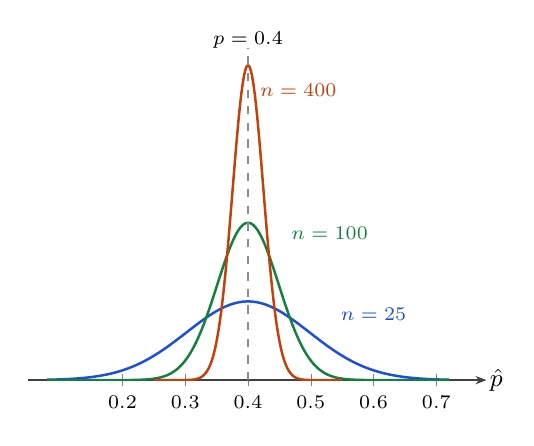
\begin{tikzpicture}[declare function={npdf(\x,\m,\s)=1/(\s*sqrt(2*pi))*exp(-((\x-\m)^2)/(2*\s^2));}]
\begin{axis}[mygraph, width=7.4cm, height=6.0cm, xmin=0.05, xmax=0.78, ymin=0, ymax=18, xtick={0.2,0.3,0.4,0.5,0.6,0.7}, ytick=\empty, axis y line=none, xlabel={$\phat$},
  every tick label/.append style={font=\scriptsize}]
  \addplot[plotA, domain=0.08:0.72, samples=200] {npdf(x,0.4,0.0980)};
  \addplot[plotC, domain=0.08:0.72, samples=200] {npdf(x,0.4,0.0490)};
  \addplot[plotB, domain=0.25:0.55, samples=200] {npdf(x,0.4,0.0245)};
  \draw[dashed, black!45] (axis cs:0.4,0) -- (axis cs:0.4,17.2);
  \node[lab, plotA] at (axis cs:0.6,3.4) {$n=25$};
  \node[lab, plotC] at (axis cs:0.53,7.6) {$n=100$};
  \node[lab, plotB] at (axis cs:0.48,15.0) {$n=400$};
  \node[lab] at (axis cs:0.4,17.6) {$p=0.4$};
\end{axis}
\end{tikzpicture}

{\scriptsize Approximate distributions of $\Phat$ when $p=0.4$. Every curve is centred at $p$, and the spread halves each time $n$ is multiplied by 4.}
\end{cols}

% -----------------------------------------------------------------
\subsection{Simulation}
\label{sec:sim}

\begin{keyres}{What simulating many random samples shows}
\begin{cols}
\begin{enumerate}
  \item $\phat$ \textbf{varies from sample to sample} (sampling variability).
  \item The values of $\phat$ are \textbf{centred on $p$}.
  \item The spread \textbf{shrinks as $n$ grows}, like $\frac{1}{\sqrt n}$.
\end{enumerate}
\nextcol
\begin{enumerate}\setcounter{enumi}{3}
  \item For large $n$ the histogram of $\phat$ is \textbf{bell-shaped} (approximately normal). For small $n$, or $p$ near $0$ or $1$, it is discrete and skewed.
  \item \textbf{Confidence intervals vary} between samples. About 95\% of 95\% intervals contain $p$.
\end{enumerate}
\end{cols}
\textbf{How:} on CAS, generate many binomial counts and divide by $n$ (e.g.\ on TI-Nspire, \texttt{randBin(n,p,k)/n} gives $k$ sample proportions), then plot a histogram. Repeat for different $n$ and $p$. Pseudocode for a simulation is in \S\ref{sec:pseudo-sim}.
\end{keyres}

% -----------------------------------------------------------------
\subsection{Confidence intervals for $p$}
\label{sec:ci}

\begin{keyres}{Approximate confidence interval (large sample)}
\[\left(\phat-z\sqrt{\frac{\phat(1-\phat)}{n}},\ \ \phat+z\sqrt{\frac{\phat(1-\phat)}{n}}\right)=(\phat-M,\ \phat+M)\]
\begin{cols}
\begin{itemize}
  \item $z$ is chosen so that $\Pr(-z<Z<z)$ is the confidence level: $90\%:\ 1.645$, \ $95\%:\ 1.96$, \ $99\%:\ 2.576$.
  \item $\sqrt{\frac{\phat(1-\phat)}{n}}$ is the (estimated) \textbf{standard error}; $M=z\sqrt{\frac{\phat(1-\phat)}{n}}$ is the \textbf{margin of error}. The width is $2M$.
  \item From an interval $(a,b)$: $\phat=\dfrac{a+b}{2}$ and $M=\dfrac{b-a}{2}$.
\end{itemize}
\nextcol
\begin{itemize}
  \item \textbf{Sample size} for a margin of error $M$: $n=\left(\frac zM\right)^2\phat(1-\phat)$, \textbf{always rounded up}. With no prior estimate, use $\phat=0.5$ (this gives the largest $n$).
  \item A \textbf{wider} interval comes from a higher confidence level or a smaller $n$. To halve the width, multiply $n$ by 4.
  \item \textbf{Claims:} a claimed value of $p$ \emph{outside} the 95\% interval is evidence against the claim; one \emph{inside} is plausible (but not proven).
\end{itemize}
\end{cols}
\end{keyres}

\begin{cols}[0.5]
\begin{warn}[Interpreting a 95\% confidence interval]
\textbf{Correct:} ``If many random samples of size $n$ were taken and a 95\% confidence interval were calculated from each, about 95\% of these intervals would contain the true population proportion $p$.''\par
\textbf{Wrong:} ``There is a 95\% probability that $p$ lies in $(0.352,0.448)$.'' Once an interval is calculated it either contains $p$ or it doesn't; $p$ is fixed, and it is the \emph{interval} that varies.\par
\textbf{Also wrong:} ``95\% of the sample lies in the interval''; ``$\phat$ lies in the interval with probability 0.95''. ($\phat$ is always the centre.)
\end{warn}
\nextcol[0.475]
\centering
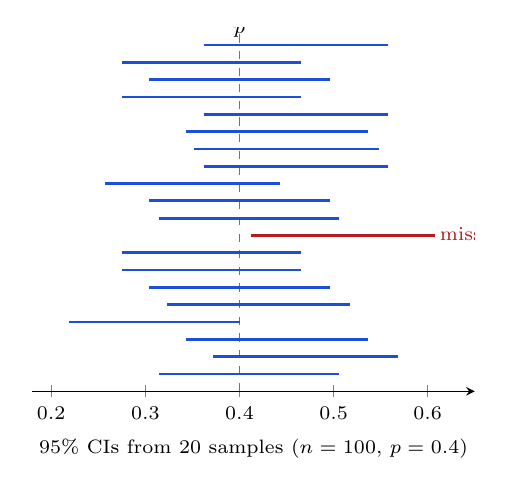
\begin{tikzpicture}
\begin{axis}[width=7.2cm, height=6.2cm, xmin=0.18, xmax=0.65, ymin=0, ymax=21, ytick=\empty, xtick={0.2,0.3,0.4,0.5,0.6},
  axis x line=bottom, axis y line=none, tick label style={font=\scriptsize}, xlabel={\scriptsize 95\% CIs from 20 samples ($n=100$, $p=0.4$)}, xlabel style={font=\scriptsize}]
  \draw[dashed, black!55] (axis cs:0.4,0) -- (axis cs:0.4,21);
  \draw[plotA, line width=1pt] (axis cs:0.314,1) -- (axis cs:0.506,1);
  \draw[plotA, line width=1pt] (axis cs:0.372,2) -- (axis cs:0.568,2);
  \draw[plotA, line width=1pt] (axis cs:0.343,3) -- (axis cs:0.537,3);
  \draw[plotA, line width=1pt] (axis cs:0.219,4) -- (axis cs:0.401,4);
  \draw[plotA, line width=1pt] (axis cs:0.323,5) -- (axis cs:0.517,5);
  \draw[plotA, line width=1pt] (axis cs:0.304,6) -- (axis cs:0.496,6);
  \draw[plotA, line width=1pt] (axis cs:0.275,7) -- (axis cs:0.465,7);
  \draw[plotA, line width=1pt] (axis cs:0.275,8) -- (axis cs:0.465,8);
  \draw[errcol, line width=1.4pt] (axis cs:0.412,9) -- (axis cs:0.608,9);
  \draw[plotA, line width=1pt] (axis cs:0.314,10) -- (axis cs:0.506,10);
  \draw[plotA, line width=1pt] (axis cs:0.304,11) -- (axis cs:0.496,11);
  \draw[plotA, line width=1pt] (axis cs:0.257,12) -- (axis cs:0.443,12);
  \draw[plotA, line width=1pt] (axis cs:0.362,13) -- (axis cs:0.558,13);
  \draw[plotA, line width=1pt] (axis cs:0.352,14) -- (axis cs:0.548,14);
  \draw[plotA, line width=1pt] (axis cs:0.343,15) -- (axis cs:0.537,15);
  \draw[plotA, line width=1pt] (axis cs:0.362,16) -- (axis cs:0.558,16);
  \draw[plotA, line width=1pt] (axis cs:0.275,17) -- (axis cs:0.465,17);
  \draw[plotA, line width=1pt] (axis cs:0.304,18) -- (axis cs:0.496,18);
  \draw[plotA, line width=1pt] (axis cs:0.275,19) -- (axis cs:0.465,19);
  \draw[plotA, line width=1pt] (axis cs:0.362,20) -- (axis cs:0.558,20);
  \node[lab, errcol, right] at (axis cs:0.608,9) {misses $p$};
  \node[lab, above] at (axis cs:0.4,20.2) {$p$};
\end{axis}
\end{tikzpicture}

{\scriptsize One simulated run: 19 of the 20 intervals contain $p$.}
\end{cols}

\begin{example}{confidence intervals}
\textbf{(a) \examtwo} In a random sample of 400 voters, 160 support a proposal. Then $\phat=\frac{160}{400}=0.4$ and the 95\% CI is $0.4\pm1.96\sqrt{\frac{0.4\times0.6}{400}}=0.4\pm0.0480$, i.e.\ $(0.352,\ 0.448)$. A claim that ``half of all voters support it'' is not supported, since $0.5$ is outside the interval.\par
\textbf{(b) \byhand} (Exam 1 style, with $z\approx2$.) $n=100$, $\phat=0.5$: \ $M\approx2\sqrt{\frac{0.5\times0.5}{100}}=2\times\frac{0.5}{10}=0.1$, so the approximate 95\% CI is $(0.4,\ 0.6)$.\par
\textbf{(c) Sample size.} For a margin of error of at most $0.03$ at 95\% confidence with $\phat\approx0.4$: $n\ge\left(\frac{1.96}{0.03}\right)^2(0.4)(0.6)\approx1024.4$, so $n=1025$. With no estimate ($\phat=0.5$): $n\ge1067.1$, so $n=1068$.\par
\textbf{(d) Working backwards.} A 95\% CI is $(0.62,\ 0.70)$. Then $\phat=0.66$, $M=0.04$ and $n\approx\left(\frac{1.96}{0.04}\right)^2(0.66)(0.34)\approx538.8$, so $n\approx539$.\par
\textbf{(e) Many intervals.} If 20 independent 95\% CIs are calculated, the number containing $p$ is $Y\sim\Bi(20,0.95)$, so $\Pr(Y\ge19)=\Pr(Y=19)+\Pr(Y=20)\approx0.736$.
\end{example}

% =================================================================
\section{Algorithms, pseudocode and technology (Outcomes 2 \& 3)}
\label{sec:algorithms}
% =================================================================

\begin{sdbox}
\textbf{Outcome 2} (emphasised in Exam 2): apply mathematical processes in non-routine contexts, including open-ended investigative, modelling or problem-solving situations. Key knowledge includes \emph{``the role of examples, counter-examples and general cases''} and \emph{``key elements of algorithm design, including sequencing, decision-making and repetition, and representations of the ordered steps for an algorithm including through the use of pseudocode''}. Skills: identify variables, constraints and key features; formulate specific and general cases; use algorithms, patterns, models and simulation; verify results; draw valid conclusions; communicate in mathematical \emph{and} everyday language.\par
\textbf{Outcome 3:} use computational thinking (abstraction, decomposition, pattern and algorithm) and the numerical, graphical, symbolic and statistical functions of technology. This covers exact vs approximate results; domain and range settings for graphs; parameters in general forms; the similarities and differences between formal mathematical expressions and their representation by technology (equivalent forms); sequencing, decision-making and repetition in algorithms and simulations; and choosing appropriate technology functions.
\end{sdbox}

\subsection{Computational thinking}
\label{sec:ct}

\begin{cols}
\begin{defn}{The four components}
\begin{itemize}
  \item \textbf{Abstraction:} keep only the essential features (e.g.\ model a tank as a cylinder).
  \item \textbf{Decomposition:} break a problem into smaller sub-problems (find the intersections, then the area, then optimise).
  \item \textbf{Pattern recognition:} spot structure (e.g.\ every member of a family passes through $(1,2)$; the derivative pattern of $f(ax+b)$).
  \item \textbf{Algorithm design:} an ordered, finite set of unambiguous steps that solves the problem (Newton's method, bisection, the trapezium rule, a simulation).
\end{itemize}
\end{defn}
\nextcol
\begin{keyres}{The modelling / problem-solving cycle}
\begin{enumerate}
  \item \textbf{Formulate:} define variables and assumptions; choose a model; set up equations.
  \item \textbf{Solve:} by hand or with technology.
  \item \textbf{Interpret:} translate results back to the context (units, sensible domain).
  \item \textbf{Verify:} check with a specific case, a graph, a substitution or a counter-example.
  \item \textbf{Communicate:} a clear conclusion in words.
\end{enumerate}
\textbf{Examples and counter-examples:} one counter-example disproves a general claim; examples (even many) do not prove one, though CAS results for general parameters can.
\end{keyres}
\end{cols}

\subsection{Pseudocode conventions \newsd}
\label{sec:pseudo}

\begin{cols}[0.5]
\begin{keyres}{Building blocks (VCAA style)}
\begin{tabular}{@{}p{2.3cm}p{5.2cm}@{}}
\textbf{Sequencing} & steps run in order, top to bottom \\
Assignment & \texttt{x $\gets$ x + 1} (store the new value in \texttt{x}) \\
\textbf{Decision} & \texttt{if} \dots\ \texttt{then} \dots\ \texttt{else} \dots\ \texttt{end if} \\
\textbf{Repetition} & \texttt{for i from 1 to n} \dots\ \texttt{end for} (a fixed number of times)\\
 & \texttt{while} condition \dots\ \texttt{end while} (until the condition is false) \\
Functions & \texttt{define f(x)} \dots\ \texttt{return} \dots \\
Output & \texttt{print x} \\
\end{tabular}
\par\smallskip
{\small Exam pseudocode is always explained in the question. Read it line by line. Conventions may vary slightly, but the logic is what is tested.}
\end{keyres}
\nextcol[0.475]
\begin{method}{Tracing pseudocode}
Make a table with one column per variable and one row per pass through the loop. Update the values \emph{in the order the lines are written}. Check the loop condition at the right moment: a \texttt{while} loop checks \emph{before} each pass.
\end{method}
\begin{example}{trace these}
\begin{minipage}[t]{0.47\linewidth}
\begin{pseudo}
a $\gets$ 1
b $\gets$ 0
for i from 1 to 4
    b $\gets$ b + a
    a $\gets$ 2 $\times$ a
end for
print b
\end{pseudo}
\end{minipage}\hfill
\begin{minipage}[t]{0.47\linewidth}
\begin{pseudo}
x $\gets$ 100
n $\gets$ 0
while x > 1
    x $\gets$ x / 3
    n $\gets$ n + 1
end while
print n
\end{pseudo}
\end{minipage}
\par\smallskip
Left: \texttt{b} takes the values $1,3,7,15$, so it prints \textbf{15}. Right: \texttt{x} goes $33.3,\,11.1,\,3.70,\,1.23,\,0.41$, so it prints \textbf{5}.
\end{example}
\end{cols}

\subsection{Standard algorithms}
\label{sec:stdalg}

\begin{cols}
\begin{keyres}{Newton's method (\S\ref*{sec:newton})}
\begin{pseudo}
define f(x) = x^3 - 2x - 5
define df(x) = 3x^2 - 2
x $\gets$ 2
change $\gets$ 1
while |change| > 0.0001
    change $\gets$ f(x) / df(x)
    x $\gets$ x - change
end while
print x                      // 2.0946
\end{pseudo}
\end{keyres}
\nextcol
\begin{keyres}{Trapezium rule (\S\ref*{sec:trap})}
\begin{pseudo}
define f(x) = x^2
a $\gets$ 0,  b $\gets$ 2,  n $\gets$ 4
h $\gets$ (b - a) / n
sum $\gets$ f(a) + f(b)
for i from 1 to n - 1
    sum $\gets$ sum + 2 $\times$ f(a + i $\times$ h)
end for
print h / 2 $\times$ sum         // 2.75
\end{pseudo}
\end{keyres}
\end{cols}

\begin{cols}
\begin{keyres}{Bisection method (a numerical solution)}
If $f$ is continuous and $f(a)$, $f(b)$ have opposite signs, there is a root in $(a,b)$. Halve the interval repeatedly, keeping the half where the sign changes.
\begin{pseudo}
while (b - a) / 2 > tolerance
    m $\gets$ (a + b) / 2
    if f(a) $\times$ f(m) < 0 then
        b $\gets$ m
    else
        a $\gets$ m
    end if
end while
print (a + b) / 2
\end{pseudo}
\end{keyres}
\nextcol
\begin{example}{bisection for $x^2-2=0$ on $[1,2]$}
\begin{tabular}{@{}ccccc@{}}
$a$ & $b$ & $m$ & $f(m)$ & keep \\ \hline
1 & 2 & 1.5 & $0.25$ & $[1,1.5]$ \\
1 & 1.5 & 1.25 & $-0.4375$ & $[1.25,1.5]$ \\
1.25 & 1.5 & 1.375 & $-0.1094$ & $[1.375,1.5]$ \\
1.375 & 1.5 & 1.4375 & $0.0664$ & $[1.375,1.4375]$ \\
\end{tabular}\par\smallskip
The root ($\sqrt2\approx1.4142$) is trapped in an interval that halves each step. Bisection is slower than Newton's method, but it always converges.
\end{example}
\end{cols}

\begin{keyres}{Simulation of sample proportions and confidence intervals}
\label{sec:pseudo-sim}
\begin{cols}[0.56]
\begin{pseudo}
p $\gets$ 0.4,  n $\gets$ 100,  count $\gets$ 0
for trial from 1 to 1000
    X $\gets$ randBin(n, p)        // successes in n trials
    phat $\gets$ X / n
    M $\gets$ 1.96 $\times$ sqrt(phat $\times$ (1 - phat) / n)
    if phat - M < p and p < phat + M then
        count $\gets$ count + 1
    end if
end for
print count / 1000                 // close to 0.95
\end{pseudo}
\nextcol[0.415]
This combines \textbf{repetition} (the \texttt{for} loop), \textbf{decision-making} (the \texttt{if}) and \textbf{sequencing}. Storing every \texttt{phat} instead would let you draw the histogram of $\Phat$ (centred at $p$, with spread $\approx\sqrt{p(1-p)/n}$). Changing \texttt{n} and \texttt{p} shows how the distribution and the interval widths change.
\end{cols}
\end{keyres}

\needspace{0.42\textheight}
\subsection{Using CAS well (Exam 2)}
\label{sec:cas}

\begin{cas}[Common tasks: check the exact syntax on your own calculator]
\small
\begin{tabularx}{\linewidth}{@{}p{3.6cm}LL@{}}
\toprule
Task & TI-Nspire CAS & Casio ClassPad \\
\midrule
Define and reuse & \texttt{Define f(x)=}\dots & \texttt{Define f(x)=}\dots \\
Solve over an interval & \texttt{solve(eqn,x)|0$\le$x$\le$2$\pi$} & \texttt{solve(eqn,x)|0$\le$x$\le$2$\pi$} \\
Numerical solution & \texttt{nSolve(eqn,x)} or graph \textsf{Intersection} & Solve in decimal mode or graph \textsf{Intersect} \\
Derivative / value & $\frac{d}{dx}$ template; \texttt{|x=a} & \texttt{diff(f(x),x)}; \texttt{|x=a} \\
Integral & $\int$ template (or \texttt{nInt}) & $\int$ template \\
Max / min on $[a,b]$ & \texttt{fMax(f(x),x,a,b)} (returns $x$) & \texttt{fMax(f(x),x,a,b)} \\
Tangent / normal & \texttt{tangentLine}, \texttt{normalLine} & \texttt{tanLine}, \texttt{normal} \\
Binomial & \texttt{binomPdf(n,p,x)}, \texttt{binomCdf(n,p,lo,hi)} & \texttt{binomialPDf(x,n,p)}, \texttt{binomialCDf(lo,hi,n,p)} \\
Normal & \texttt{normCdf(lo,hi,$\mu$,$\sigma$)}, \texttt{invNorm(area,$\mu$,$\sigma$)} & \texttt{normCDf(lo,hi,$\sigma$,$\mu$)} ($\sigma$ \emph{first}), \texttt{invNormCDf("L",area,$\sigma$,$\mu$)} \\
Random samples & \texttt{randBin(n,p,k)} & \texttt{randBin(n,p,k)} \\
\bottomrule
\end{tabularx}
\end{cas}

\begin{cols}
\begin{tip}[Exact vs approximate; CAS vs written notation]
\begin{itemize}
  \item Keep CAS in \textbf{radian} and \textbf{exact} (standard) mode unless you need decimals. Store intermediate results instead of retyping rounded values.
  \item CAS writes $\ln$ for $\loge$, may write $\frac{1}{\cos^2x}$ as $\sec^2x$, and gives equivalent forms (e.g.\ $\frac12\loge\left(\frac{x+1}{3}\right)$ vs $\frac{\loge(x+1)-\loge3}{2}$). Both are fine. Write answers in \textbf{standard mathematical notation}, never calculator syntax (not \texttt{e\^{}(2x)} or \texttt{sqrt(}).
  \item CAS general solutions use \texttt{n1}, \texttt{constn} etc. Write $k\in\Z$.
  \item Choose a sensible viewing window (domain and range) so all key features show; check for hidden intersections or asymptotes.
\end{itemize}
\end{tip}
\nextcol
\begin{tip}[Getting the most from technology]
\begin{itemize}
  \item \textbf{Parameters:} define $f(x)$ with a parameter $k$, then solve for $k$ (e.g.\ ``the tangent at $x=1$ passes through the origin''). Graph several values of $k$ to see the family.
  \item \textbf{Verify} by substitution, by graphing both sides, or by differentiating an anti-derivative.
  \item \textbf{Constraints:} use \texttt{|} to restrict domains (e.g.\ $x>0$, $0\le t\le24$) and remove extraneous solutions.
  \item In ``show that'' questions CAS output alone is not enough. Write the algebraic steps.
\end{itemize}
\end{tip}
\end{cols}

% =================================================================
\section{Exam technique and the errors that cost marks}
\label{sec:technique}
% =================================================================

\begin{tip}[What examiners keep saying (themes from VCAA examination reports)]
\begin{itemize}
  \item \textbf{Show the key step.} In Exam 1, and in Exam 2 questions worth more than 1 mark, an answer alone often earns only part of the marks. Write the equation you are solving, the derivative or the integral with its bounds.
  \item \textbf{Use correct notation.} $\dydx=\dots$ or $f'(x)=\dots$, not ``$=$'' chains joining unequal things; integrals need $dx$; indefinite integrals need $+c$; write $\loge$, not calculator syntax; use set and interval notation correctly.
  \item \textbf{Answer the actual question.} Give coordinates when asked for a point, the \emph{value} when asked for the maximum value (not the $x$ where it occurs), all values of a parameter when asked for ``values'', units, and a sentence in context.
  \item \textbf{Exact means exact.} When decimals are asked for, round only at the end and to the stated accuracy.
  \item \textbf{``Hence''} means use the previous part. ``Show that'' means every step to the given answer, with no gaps.
\end{itemize}
\end{tip}

\subsection{Topic-by-topic errors to avoid}

\begin{warn}[Functions and graphs]
\begin{multicols}{2}
\begin{itemize}
  \item Missing asymptote equations, open/closed endpoints, or coordinates on sketches.
  \item Graphs that bend the wrong way near asymptotes or cross an asymptote they can't (e.g.\ $y=e^x$ crossing $y=0$).
  \item Dilation factor: $f(2x)$ is a factor of $\frac12$ from the $y$-axis. Translation direction: $f(x+3)$ moves \emph{left}.
  \item Doing transformations in the wrong order, or not factorising inside the brackets before reading off.
  \item Writing $f^{-1}$ for $\frac1f$; forgetting the domain of $f^{-1}$ (it is the range of $f$).
  \item Composite domain: $d_{f\circ g}=d_g$, not the implied domain of the simplified rule.
  \item CAS in degree mode.
\end{itemize}
\end{multicols}
\end{warn}
\begin{warn}[Algebra and equations]
\begin{multicols}{2}
\begin{itemize}
  \item Missing solutions in circular equations because the interval for $ax+b$ wasn't adjusted.
  \item Dividing by an expression that might be zero (e.g.\ $\sin x$) and losing solutions. Factorise instead.
  \item Not rejecting invalid solutions of log equations (check that every argument is $>0$).
  \item $\loge(a+b)\ne\loge a+\loge b$; \ $e^{x+y}=e^xe^y$.
  \item Simultaneous equations: when the determinant is $0$, you still have to check whether there are no solutions or infinitely many.
  \item The $k=0$ case in ``$kx^2+\dots$'' (it is not a quadratic then).
\end{itemize}
\end{multicols}
\end{warn}
\begin{warn}[Calculus]
\begin{multicols}{2}
\begin{itemize}
  \item Forgetting the inner derivative in the chain rule ($\ddx e^{3x}=3e^{3x}$).
  \item Quotient rule in the wrong order: it is $\frac{vu'-uv'}{v^2}$.
  \item $\int\frac{1}{ax+b}\dx=\frac1a\loge(ax+b)+c$ ($ax+b>0$): don't drop the $\frac1a$. Likewise $\int\sin(ax)\dx=-\frac1a\cos(ax)$: watch the sign.
  \item Integrating across an $x$-intercept and calling the signed integral the ``area''.
  \item Area between curves: use top minus bottom, and split where the curves cross.
  \item Confusing the average value $\frac{1}{b-a}\int_a^bf$ with the average rate of change $\frac{f(b)-f(a)}{b-a}$.
  \item Not justifying the nature of a stationary point; ignoring endpoints for absolute max/min.
  \item Strictly increasing intervals that join across an asymptote or point of discontinuity.
  \item Trapezium rule: wrong strip width $h$, or not doubling the interior values. Newton's method: rounding $x_n$ too early.
\end{itemize}
\end{multicols}
\end{warn}
\begin{warn}[Probability and statistics]
\begin{multicols}{2}
\begin{itemize}
  \item $\Nd(\mu,\sigma^2)$: the second parameter is the \emph{variance}. Enter $\sigma$ (not $\sigma^2$) into CAS.
  \item Discrete inequalities: $\Pr(X>2)=1-\Pr(X\le2)$, not $1-\Pr(X\le3)$.
  \item Conditional probability: the denominator is the probability of the \emph{given} event.
  \item Using the binomial distribution when the trials aren't independent (sampling without replacement), or not stating the binomial conditions when asked to justify.
  \item pdf questions: checking only one condition; mixing up the median (area $0.5$) and the mean ($\int xf(x)\dx$).
  \item Confidence intervals: incorrect interpretation; rounding $n$ \emph{down} (always round up); using the normal approximation when the question says to use the binomial (or vice versa).
\end{itemize}
\end{multicols}
\end{warn}

\subsection{Typical question types}

\begin{cols}
\begin{keyres}{Exam 1 (no technology): practise until automatic}
\begin{itemize}
  \item Differentiate (product, quotient, chain) and evaluate at a point.
  \item ``Differentiate \dots\ hence find an anti-derivative of \dots''
  \item Anti-derivatives of $f(ax+b)$; definite integrals with exact values; area between curves.
  \item Solve a circular, exponential or log equation exactly over an interval.
  \item Inverse and composite functions with domains and ranges.
  \item Sketch a transformed exponential, log, power or polynomial graph with features labelled.
  \item Tangent and normal lines; stationary points; a simple optimisation.
  \item Discrete table with an unknown, mean and variance; binomial with small $n$; pdf: find $k$, a probability, a median; normal symmetry using given probabilities; small-sample $\Phat$; CI with $z\approx2$.
  \item Simultaneous equations with a parameter; one or two steps of Newton's method; the trapezium rule; trace pseudocode.
\end{itemize}
\end{keyres}
\nextcol
\begin{keyres}{Exam 2 (CAS): what Section B usually looks like}
\begin{itemize}
  \item \textbf{Function and calculus modelling:} a curve, track, tank or population model. Find features, rates and optimal values; areas; join curves smoothly (hybrid functions).
  \item \textbf{Circular modelling:} tides, temperature or a Ferris wheel. Find amplitude, period and translations; solve equations for times; average values.
  \item \textbf{Probability:} discrete $\to$ binomial $\to$ continuous pdf $\to$ normal $\to$ sample proportions and CIs, often linked through one context, with conditional probability.
  \item \textbf{Families and parameters:} a function with a parameter $a$ or $k$. Find the values for which there are $n$ solutions, a tangent, an inverse, etc.
  \item \textbf{Transformations and inverses} combined with calculus (e.g.\ the area between $f$ and $f^{-1}$).
\end{itemize}
\textbf{Section A (MCQ):} quick checks by graphing, substituting the options, or testing special values. About 1.5 minutes each.
\end{keyres}
\end{cols}

\begin{tip}[Final-week routine]
\begin{enumerate}
  \item Do full past exams under timed conditions. VCAA papers from 2023 onwards match this study design. Older papers (2016--2022) are still good practice for most topics: check any unfamiliar question against the checklist in Section~\ref{sec:checklist}.
  \item Read the matching VCAA examination report for each paper. It lists exactly where marks were lost.
  \item Re-do every question you got wrong 2--3 days later, without looking.
  \item For Exam 2, finalise your bound reference: this sheet, CAS syntax notes and your own worked solutions. Tab it by topic so you can find things in seconds.
  \item Use the checklist in the next section to find your last gaps.
\end{enumerate}
\end{tip}

% =================================================================
\section{Study design checklist: every dot point, where it is covered}
\label{sec:checklist}
% =================================================================

Tick each item when you can do it \emph{without notes} (for \byhand\ items) or quickly with CAS. ``Where'' gives the section and page of this sheet. Every dot point and key skill in the study design for Units 3 and 4 Mathematical Methods is listed.

\newcommand{\cl}[3]{\checkbox & #1 & \S\ref{#2} & p.\,\pageref{#2}#3\\}
\newcommand{\clhead}[1]{\multicolumn{4}{@{}l}{\cellcolor{navy}\color{white}\sffamily\bfseries\small #1}\\}
\newcommand{\cltablestart}{\small\renewcommand{\arraystretch}{1.25}\begin{tabularx}{\linewidth}{@{}c@{\hspace{6pt}}Lll@{}}}

\cltablestart
\clhead{Area of Study 1: Functions, relations and graphs}
\cl{Graphs of polynomial functions and their key features}{sec:poly}{}
\cl{Power functions $y=x^n$, $n\in\Q$: domains, ranges, asymptotes, symmetry}{sec:power}{}
\cl{Exponential $y=a^x$ ($a\in\R^+$), especially $y=e^x$; logarithmic $y=\loge(x)$, $y=\log_{10}(x)$}{sec:explog}{}
\cl{Circular functions $\sin$, $\cos$, $\tan$: amplitude, period, asymptotes, key features}{sec:circ}{}
\cl{Transformation $y=f(x)\to y=Af(n(x+b))+c$ and the inverse transformation; the mapping of points}{sec:trans}{}
\cl{Relation between original and transformed graphs; families with one parameter}{sec:families}{}
\cl{Graphs of sums, differences, products and composites (not reciprocal/quotient composites)}{sec:combo}{}
\cl{Hybrid (piecewise) functions: sketching, continuity at the joins}{sec:hybrid}{}
\cl{Modelling with polynomial, power, circular, exponential and log functions; recognising models from graphs or tables}{sec:model}{}
\cl{Domain (maximal/implied), co-domain, range, asymptotic behaviour, symmetry}{sec:domain}{}
\cl{\byhand\ sketch polynomials (degree $\le4$), $x^n$ ($n\in\N$), $a^x$ (via $(-1,\frac1a)$, $(0,1)$, $(1,a)$), $\loge x$, $\log_{10}x$ and simple transformations}{sec:poly}{}
\cl{Exponent (index) laws and logarithm laws; simplifying expressions}{sec:explog}{}
\end{tabularx}

\medskip
\cltablestart
\clhead{Area of Study 2: Algebra, number and structure}
\cl{Polynomial equations of degree $n$ (up to $n$ real solutions), including numerical solutions}{sec:polyeq}{}
\cl{Inverse functions: existence (one-to-one), rule, domain and range, graph (reflection in $y=x$)}{sec:inverse}{}
\cl{Using inverse functions to solve exponential, logarithmic, circular and power equations}{sec:solve}{}
\cl{Composite functions $f\circ g$ (exists iff $r_g\subseteq d_f$): rule, domain and range}{sec:composite}{}
\cl{Solving $f(x)=g(x)$ over an interval: algebraic, graphical and numerical methods}{sec:solve}{}
\cl{\byhand\ $\sin(ax+b)=c$, $\cos(ax+b)=c$, $\tan(ax+b)=c$ exactly over an interval; general solutions}{sec:circeq}{}
\cl{Literal equations; general solutions of equations with a single parameter}{sec:literal}{}
\cl{Simultaneous linear equations: unique, none or infinitely many solutions (2 lines geometrically)}{sec:simul}{}
\cl{Numerical methods: Newton's method (algorithm), bisection; verifying solutions}{sec:newton}{}
\cl{Properties of functions and functional equations}{sec:funceq}{}
\end{tabularx}

\medskip
\cltablestart
\clhead{Area of Study 3: Calculus}
\cl{Graphical treatment of limits, continuity and differentiability}{sec:cont}{}
\cl{Deducing the graph of the derivative from the graph of a function}{sec:gradgraph}{}
\cl{Deducing the graph of an anti-derivative from the graph of a function}{sec:antigraph}{}
\cl{Derivatives of $x^n$ ($n\in\Q$), $e^x$, $\loge(x)$, $\sin x$, $\cos x$, $\tan x$, and of $f(ax+b)$}{sec:rules}{}
\cl{\byhand\ sum, difference, product, quotient and chain rules}{sec:rules}{}
\cl{Tangents (and normals) to a curve at a given point}{sec:tangent}{}
\cl{Graph sketching: stationary points, points of inflection, strictly increasing/decreasing intervals}{sec:sp}{}
\cl{Curve sketching with calculus (all key features)}{sec:sketch}{}
\cl{Local and absolute max/min over an interval (including endpoints); optimisation in context}{sec:opt}{}
\cl{Rates of change in context}{sec:rates}{}
\cl{\byhand\ anti-derivatives of polynomials, power functions and $f(ax+b)$ for $x^n$, $e^x$, $\sin$, $\cos$}{sec:antideriv}{}
\cl{Anti-differentiation by recognition ($F'=f\Rightarrow\int f\dx=F+c$)}{sec:recog}{}
\cl{Fundamental theorem of calculus $\int_a^bf(x)\dx=F(b)-F(a)$; properties of definite integrals}{sec:definite}{}
\cl{Definite integral as a limit of sums; trapezium rule approximation}{sec:trap}{}
\cl{Finding a function from its rate of change and a boundary condition}{sec:bc}{}
\cl{Area under a curve and between curves}{sec:area}{}
\cl{Average value of a function}{sec:avg}{}
\cl{Other applications (net change, motion, probability)}{sec:apps}{}
\end{tabularx}

\medskip
\cltablestart
\clhead{Area of Study 4: Data analysis, probability and statistics}
\cl{Random variable as a real function on a sample space; discrete vs continuous}{sec:rvdef}{}
\cl{Discrete distributions via graphs, tables, pmfs; mean, variance, standard deviation}{sec:discrete}{}
\cl{Bernoulli trials and $\Bi(n,p)$; conditions for using a binomial model}{sec:binomial}{}
\cl{Effect of the parameters on the graph of a pmf}{sec:binomial}{}
\cl{Probabilities of values and intervals, including conditional probability (discrete)}{sec:discrete}{}
\cl{Constructing a pdf from a non-negative function (finding $k$)}{sec:crv}{}
\cl{pdfs: probabilities, mean, variance, standard deviation, median, mode}{sec:crv}{}
\cl{Effect of the parameters on the graph of a pdf}{sec:crv}{}
\cl{Standard normal $\Nd(0,1)$ and $\Nd(\mu,\sigma^2)$: standardising, symmetry, inverse normal}{sec:normal}{}
\cl{Probabilities of intervals, including conditional probability (continuous)}{sec:normal}{}
\cl{Population parameter vs sample statistic; estimating $p$ with $\phat$}{sec:popsamp}{}
\cl{$\Phat=\frac Xn$ as a random variable; exact distribution for small $n$}{sec:phat}{}
\cl{Approximate normality of $\Phat$ for large $n$: mean $p$, standard deviation $\sqrt{p(1-p)/n}$}{sec:phat}{}
\cl{Simulation of random sampling: distribution of $\Phat$, variation in confidence intervals}{sec:sim}{}
\cl{Approximate confidence intervals (95\% with $z\approx1.96$), interpretation, margin of error, sample size}{sec:ci}{}
\end{tabularx}

\medskip
\cltablestart
\clhead{Outcomes 2 and 3: problem solving, algorithms and technology}
\cl{Computational thinking: abstraction, decomposition, pattern, algorithm; the modelling cycle}{sec:ct}{}
\cl{Algorithm design (sequencing, decision-making, repetition) and pseudocode; tracing}{sec:pseudo}{}
\cl{Standard algorithms: Newton's method, bisection, trapezium rule, simulation}{sec:stdalg}{}
\cl{Exact vs approximate results; technology notation vs formal notation; choosing CAS functions}{sec:cas}{}
\cl{Examples, counter-examples and general cases; verifying results}{sec:ct}{}
\cl{Exam conditions, the formula sheet and command terms}{sec:exam}{}
\end{tabularx}

\vfill
\begin{tcolorbox}[basebox, colback=sdbg, colframe=sdcol, title={\faInfoCircle\enspace About this sheet}]
\small Prepared from the VCAA \emph{VCE Mathematics Study Design 2023--2027} (Units 3 and 4: Mathematical Methods, version 1.1). Every worked example in this sheet was checked independently with a computer algebra system. Exam structures (marks, sections) are those of the 2023--2025 VCAA examinations. Always confirm the current examination specifications and formula sheet on the VCAA website.
\end{tcolorbox}


\end{document}
